\documentclass{article}

% if you need to pass options to natbib, use, e.g.:
%     \PassOptionsToPackage{numbers, compress}{natbib}
% before loading neurips_2026

% ==========================================
% 1. NeurIPS 2026 Setup
% ==========================================
% The authors should use one of these tracks.
% Before accepting by the NeurIPS conference, select one of the options below.
% 0. "default" for submission
\usepackage{neurips_2026}
% the "default" option is equal to the "main" option, which is used for the Main Track with double-blind reviewing.
% 1. "main" option is used for the Main Track
%  \usepackage[main]{neurips_2026}
% 2. "position" option is used for the Position Paper Track
%  \usepackage[position]{neurips_2026}
% 3. "eandd" option is used for the Evaluations & Datasets Track
 % \usepackage[eandd]{neurips_2026}
% 4. "creativeai" option is used for the Creative AI Track
%  \usepackage[creativeai]{neurips_2026}
% 5. "sglblindworkshop" option is used for the Workshop with single-blind reviewing
 % \usepackage[sglblindworkshop]{neurips_2026}
% 6. "dblblindworkshop" option is used for the Workshop with double-blind reviewing
%  \usepackage[dblblindworkshop]{neurips_2026}

% After being accepted, the authors should add "final" behind the track to compile a camera-ready version.
% 1. Main Track
 % \usepackage[main, final]{neurips_2026}
% 2. Position Paper Track
%  \usepackage[position, final]{neurips_2026}
% 3. Evaluations & Datasets Track
 % \usepackage[eandd, final]{neurips_2026}
% 4. Creative AI Track
%  \usepackage[creativeai, final]{neurips_2026}
% 5. Workshop with single-blind reviewing
%  \usepackage[sglblindworkshop, final]{neurips_2026}
% 6. Workshop with double-blind reviewing
%  \usepackage[dblblindworkshop, final]{neurips_2026}
% Note. For the workshop paper template, both \title{} and \workshoptitle{} are required, with the former indicating the paper title shown in the title and the latter indicating the workshop title displayed in the footnote.
% For workshops (5., 6.), the authors should add the name of the workshop, "\workshoptitle" command is used to set the workshop title.
% \workshoptitle{WORKSHOP TITLE}

% "preprint" option is used for arXiv or other preprint submissions
 % \usepackage[preprint]{neurips_2026}

% to avoid loading the natbib package, add option nonatbib:
%    \usepackage[nonatbib]{neurips_2026}

% ==========================================
% 2. Core & Typography
% ==========================================
\usepackage[utf8]{inputenc} % allow utf-8 input
\usepackage[T1]{fontenc}    % use 8-bit T1 fonts
\usepackage{times}          % Times font
\usepackage{latexsym}       % standard latex symbols
\usepackage{microtype}      % microtypography

% ==========================================
% 3. Colors & Graphics
% ==========================================
% NOTE: Load xcolor early with options to avoid "Option clash" errors
\usepackage[table,xcdraw]{xcolor} 
\usepackage{wrapfig}        % for wrapfigure
\usepackage{graphicx}       % for resizebox
\usepackage{caption}
\usepackage{subcaption}

% ==========================================
% 4. Math
% ==========================================
\usepackage{amsmath,amsfonts,bm}
\usepackage{mathtools}      % Required in preamble
\usepackage{nicefrac}       % compact symbols for 1/2, etc.
\usepackage{cuted}          % formula autolining
%%%%% NEW MATH DEFINITIONS %%%%%

\usepackage{amsmath,amsfonts,bm}

% Mark sections of captions for referring to divisions of figures
\newcommand{\figleft}{{\em (Left)}}
\newcommand{\figcenter}{{\em (Center)}}
\newcommand{\figright}{{\em (Right)}}
\newcommand{\figtop}{{\em (Top)}}
\newcommand{\figbottom}{{\em (Bottom)}}
\newcommand{\captiona}{{\em (a)}}
\newcommand{\captionb}{{\em (b)}}
\newcommand{\captionc}{{\em (c)}}
\newcommand{\captiond}{{\em (d)}}

% Highlight a newly defined term
\newcommand{\newterm}[1]{{\bf #1}}


% Figure reference, lower-case.
\def\figref#1{figure~\ref{#1}}
% Figure reference, capital. For start of sentence
\def\Figref#1{Figure~\ref{#1}}
\def\twofigref#1#2{figures \ref{#1} and \ref{#2}}
\def\quadfigref#1#2#3#4{figures \ref{#1}, \ref{#2}, \ref{#3} and \ref{#4}}
% Section reference, lower-case.
\def\secref#1{section~\ref{#1}}
% Section reference, capital.
\def\Secref#1{Section~\ref{#1}}
% Reference to two sections.
\def\twosecrefs#1#2{sections \ref{#1} and \ref{#2}}
% Reference to three sections.
\def\secrefs#1#2#3{sections \ref{#1}, \ref{#2} and \ref{#3}}
% Reference to an equation, lower-case.
\def\eqref#1{equation~\ref{#1}}
% Reference to an equation, upper case
\def\Eqref#1{Equation~\ref{#1}}
% A raw reference to an equation---avoid using if possible
\def\plaineqref#1{\ref{#1}}
% Reference to a chapter, lower-case.
\def\chapref#1{chapter~\ref{#1}}
% Reference to an equation, upper case.
\def\Chapref#1{Chapter~\ref{#1}}
% Reference to a range of chapters
\def\rangechapref#1#2{chapters\ref{#1}--\ref{#2}}
% Reference to an algorithm, lower-case.
\def\algref#1{algorithm~\ref{#1}}
% Reference to an algorithm, upper case.
\def\Algref#1{Algorithm~\ref{#1}}
\def\twoalgref#1#2{algorithms \ref{#1} and \ref{#2}}
\def\Twoalgref#1#2{Algorithms \ref{#1} and \ref{#2}}
% Reference to a part, lower case
\def\partref#1{part~\ref{#1}}
% Reference to a part, upper case
\def\Partref#1{Part~\ref{#1}}
\def\twopartref#1#2{parts \ref{#1} and \ref{#2}}

\def\ceil#1{\lceil #1 \rceil}
\def\floor#1{\lfloor #1 \rfloor}
\def\1{\bm{1}}
\newcommand{\train}{\mathcal{D}}
\newcommand{\valid}{\mathcal{D_{\mathrm{valid}}}}
\newcommand{\test}{\mathcal{D_{\mathrm{test}}}}

\def\eps{{\epsilon}}


% Random variables
\def\reta{{\textnormal{$\eta$}}}
\def\ra{{\textnormal{a}}}
\def\rb{{\textnormal{b}}}
\def\rc{{\textnormal{c}}}
\def\rd{{\textnormal{d}}}
\def\re{{\textnormal{e}}}
\def\rf{{\textnormal{f}}}
\def\rg{{\textnormal{g}}}
\def\rh{{\textnormal{h}}}
\def\ri{{\textnormal{i}}}
\def\rj{{\textnormal{j}}}
\def\rk{{\textnormal{k}}}
\def\rl{{\textnormal{l}}}
% rm is already a command, just don't name any random variables m
\def\rn{{\textnormal{n}}}
\def\ro{{\textnormal{o}}}
\def\rp{{\textnormal{p}}}
\def\rq{{\textnormal{q}}}
\def\rr{{\textnormal{r}}}
\def\rs{{\textnormal{s}}}
\def\rt{{\textnormal{t}}}
\def\ru{{\textnormal{u}}}
\def\rv{{\textnormal{v}}}
\def\rw{{\textnormal{w}}}
\def\rx{{\textnormal{x}}}
\def\ry{{\textnormal{y}}}
\def\rz{{\textnormal{z}}}

% Random vectors
\def\rvepsilon{{\mathbf{\epsilon}}}
\def\rvtheta{{\mathbf{\theta}}}
\def\rva{{\mathbf{a}}}
\def\rvb{{\mathbf{b}}}
\def\rvc{{\mathbf{c}}}
\def\rvd{{\mathbf{d}}}
\def\rve{{\mathbf{e}}}
\def\rvf{{\mathbf{f}}}
\def\rvg{{\mathbf{g}}}
\def\rvh{{\mathbf{h}}}
\def\rvu{{\mathbf{i}}}
\def\rvj{{\mathbf{j}}}
\def\rvk{{\mathbf{k}}}
\def\rvl{{\mathbf{l}}}
\def\rvm{{\mathbf{m}}}
\def\rvn{{\mathbf{n}}}
\def\rvo{{\mathbf{o}}}
\def\rvp{{\mathbf{p}}}
\def\rvq{{\mathbf{q}}}
\def\rvr{{\mathbf{r}}}
\def\rvs{{\mathbf{s}}}
\def\rvt{{\mathbf{t}}}
\def\rvu{{\mathbf{u}}}
\def\rvv{{\mathbf{v}}}
\def\rvw{{\mathbf{w}}}
\def\rvx{{\mathbf{x}}}
\def\rvy{{\mathbf{y}}}
\def\rvz{{\mathbf{z}}}

% Elements of random vectors
\def\erva{{\textnormal{a}}}
\def\ervb{{\textnormal{b}}}
\def\ervc{{\textnormal{c}}}
\def\ervd{{\textnormal{d}}}
\def\erve{{\textnormal{e}}}
\def\ervf{{\textnormal{f}}}
\def\ervg{{\textnormal{g}}}
\def\ervh{{\textnormal{h}}}
\def\ervi{{\textnormal{i}}}
\def\ervj{{\textnormal{j}}}
\def\ervk{{\textnormal{k}}}
\def\ervl{{\textnormal{l}}}
\def\ervm{{\textnormal{m}}}
\def\ervn{{\textnormal{n}}}
\def\ervo{{\textnormal{o}}}
\def\ervp{{\textnormal{p}}}
\def\ervq{{\textnormal{q}}}
\def\ervr{{\textnormal{r}}}
\def\ervs{{\textnormal{s}}}
\def\ervt{{\textnormal{t}}}
\def\ervu{{\textnormal{u}}}
\def\ervv{{\textnormal{v}}}
\def\ervw{{\textnormal{w}}}
\def\ervx{{\textnormal{x}}}
\def\ervy{{\textnormal{y}}}
\def\ervz{{\textnormal{z}}}

% Random matrices
\def\rmA{{\mathbf{A}}}
\def\rmB{{\mathbf{B}}}
\def\rmC{{\mathbf{C}}}
\def\rmD{{\mathbf{D}}}
\def\rmE{{\mathbf{E}}}
\def\rmF{{\mathbf{F}}}
\def\rmG{{\mathbf{G}}}
\def\rmH{{\mathbf{H}}}
\def\rmI{{\mathbf{I}}}
\def\rmJ{{\mathbf{J}}}
\def\rmK{{\mathbf{K}}}
\def\rmL{{\mathbf{L}}}
\def\rmM{{\mathbf{M}}}
\def\rmN{{\mathbf{N}}}
\def\rmO{{\mathbf{O}}}
\def\rmP{{\mathbf{P}}}
\def\rmQ{{\mathbf{Q}}}
\def\rmR{{\mathbf{R}}}
\def\rmS{{\mathbf{S}}}
\def\rmT{{\mathbf{T}}}
\def\rmU{{\mathbf{U}}}
\def\rmV{{\mathbf{V}}}
\def\rmW{{\mathbf{W}}}
\def\rmX{{\mathbf{X}}}
\def\rmY{{\mathbf{Y}}}
\def\rmZ{{\mathbf{Z}}}

% Elements of random matrices
\def\ermA{{\textnormal{A}}}
\def\ermB{{\textnormal{B}}}
\def\ermC{{\textnormal{C}}}
\def\ermD{{\textnormal{D}}}
\def\ermE{{\textnormal{E}}}
\def\ermF{{\textnormal{F}}}
\def\ermG{{\textnormal{G}}}
\def\ermH{{\textnormal{H}}}
\def\ermI{{\textnormal{I}}}
\def\ermJ{{\textnormal{J}}}
\def\ermK{{\textnormal{K}}}
\def\ermL{{\textnormal{L}}}
\def\ermM{{\textnormal{M}}}
\def\ermN{{\textnormal{N}}}
\def\ermO{{\textnormal{O}}}
\def\ermP{{\textnormal{P}}}
\def\ermQ{{\textnormal{Q}}}
\def\ermR{{\textnormal{R}}}
\def\ermS{{\textnormal{S}}}
\def\ermT{{\textnormal{T}}}
\def\ermU{{\textnormal{U}}}
\def\ermV{{\textnormal{V}}}
\def\ermW{{\textnormal{W}}}
\def\ermX{{\textnormal{X}}}
\def\ermY{{\textnormal{Y}}}
\def\ermZ{{\textnormal{Z}}}

% Vectors
\def\vzero{{\bm{0}}}
\def\vone{{\bm{1}}}
\def\vmu{{\bm{\mu}}}
\def\vtheta{{\bm{\theta}}}
\def\va{{\bm{a}}}
\def\vb{{\bm{b}}}
\def\vc{{\bm{c}}}
\def\vd{{\bm{d}}}
\def\ve{{\bm{e}}}
\def\vf{{\bm{f}}}
\def\vg{{\bm{g}}}
\def\vh{{\bm{h}}}
\def\vi{{\bm{i}}}
\def\vj{{\bm{j}}}
\def\vk{{\bm{k}}}
\def\vl{{\bm{l}}}
\def\vm{{\bm{m}}}
\def\vn{{\bm{n}}}
\def\vo{{\bm{o}}}
\def\vp{{\bm{p}}}
\def\vq{{\bm{q}}}
\def\vr{{\bm{r}}}
\def\vs{{\bm{s}}}
\def\vt{{\bm{t}}}
\def\vu{{\bm{u}}}
\def\vv{{\bm{v}}}
\def\vw{{\bm{w}}}
\def\vx{{\bm{x}}}
\def\vy{{\bm{y}}}
\def\vz{{\bm{z}}}

% Elements of vectors
\def\evalpha{{\alpha}}
\def\evbeta{{\beta}}
\def\evepsilon{{\epsilon}}
\def\evlambda{{\lambda}}
\def\evomega{{\omega}}
\def\evmu{{\mu}}
\def\evpsi{{\psi}}
\def\evsigma{{\sigma}}
\def\evtheta{{\theta}}
\def\eva{{a}}
\def\evb{{b}}
\def\evc{{c}}
\def\evd{{d}}
\def\eve{{e}}
\def\evf{{f}}
\def\evg{{g}}
\def\evh{{h}}
\def\evi{{i}}
\def\evj{{j}}
\def\evk{{k}}
\def\evl{{l}}
\def\evm{{m}}
\def\evn{{n}}
\def\evo{{o}}
\def\evp{{p}}
\def\evq{{q}}
\def\evr{{r}}
\def\evs{{s}}
\def\evt{{t}}
\def\evu{{u}}
\def\evv{{v}}
\def\evw{{w}}
\def\evx{{x}}
\def\evy{{y}}
\def\evz{{z}}

% Matrix
\def\mA{{\bm{A}}}
\def\mB{{\bm{B}}}
\def\mC{{\bm{C}}}
\def\mD{{\bm{D}}}
\def\mE{{\bm{E}}}
\def\mF{{\bm{F}}}
\def\mG{{\bm{G}}}
\def\mH{{\bm{H}}}
\def\mI{{\bm{I}}}
\def\mJ{{\bm{J}}}
\def\mK{{\bm{K}}}
\def\mL{{\bm{L}}}
\def\mM{{\bm{M}}}
\def\mN{{\bm{N}}}
\def\mO{{\bm{O}}}
\def\mP{{\bm{P}}}
\def\mQ{{\bm{Q}}}
\def\mR{{\bm{R}}}
\def\mS{{\bm{S}}}
\def\mT{{\bm{T}}}
\def\mU{{\bm{U}}}
\def\mV{{\bm{V}}}
\def\mW{{\bm{W}}}
\def\mX{{\bm{X}}}
\def\mY{{\bm{Y}}}
\def\mZ{{\bm{Z}}}
\def\mBeta{{\bm{\beta}}}
\def\mPhi{{\bm{\Phi}}}
\def\mLambda{{\bm{\Lambda}}}
\def\mSigma{{\bm{\Sigma}}}

% Tensor
\DeclareMathAlphabet{\mathsfit}{\encodingdefault}{\sfdefault}{m}{sl}
\SetMathAlphabet{\mathsfit}{bold}{\encodingdefault}{\sfdefault}{bx}{n}
\newcommand{\tens}[1]{\bm{\mathsfit{#1}}}
\def\tA{{\tens{A}}}
\def\tB{{\tens{B}}}
\def\tC{{\tens{C}}}
\def\tD{{\tens{D}}}
\def\tE{{\tens{E}}}
\def\tF{{\tens{F}}}
\def\tG{{\tens{G}}}
\def\tH{{\tens{H}}}
\def\tI{{\tens{I}}}
\def\tJ{{\tens{J}}}
\def\tK{{\tens{K}}}
\def\tL{{\tens{L}}}
\def\tM{{\tens{M}}}
\def\tN{{\tens{N}}}
\def\tO{{\tens{O}}}
\def\tP{{\tens{P}}}
\def\tQ{{\tens{Q}}}
\def\tR{{\tens{R}}}
\def\tS{{\tens{S}}}
\def\tT{{\tens{T}}}
\def\tU{{\tens{U}}}
\def\tV{{\tens{V}}}
\def\tW{{\tens{W}}}
\def\tX{{\tens{X}}}
\def\tY{{\tens{Y}}}
\def\tZ{{\tens{Z}}}


% Graph
\def\gA{{\mathcal{A}}}
\def\gB{{\mathcal{B}}}
\def\gC{{\mathcal{C}}}
\def\gD{{\mathcal{D}}}
\def\gE{{\mathcal{E}}}
\def\gF{{\mathcal{F}}}
\def\gG{{\mathcal{G}}}
\def\gH{{\mathcal{H}}}
\def\gI{{\mathcal{I}}}
\def\gJ{{\mathcal{J}}}
\def\gK{{\mathcal{K}}}
\def\gL{{\mathcal{L}}}
\def\gM{{\mathcal{M}}}
\def\gN{{\mathcal{N}}}
\def\gO{{\mathcal{O}}}
\def\gP{{\mathcal{P}}}
\def\gQ{{\mathcal{Q}}}
\def\gR{{\mathcal{R}}}
\def\gS{{\mathcal{S}}}
\def\gT{{\mathcal{T}}}
\def\gU{{\mathcal{U}}}
\def\gV{{\mathcal{V}}}
\def\gW{{\mathcal{W}}}
\def\gX{{\mathcal{X}}}
\def\gY{{\mathcal{Y}}}
\def\gZ{{\mathcal{Z}}}

% Sets
\def\sA{{\mathbb{A}}}
\def\sB{{\mathbb{B}}}
\def\sC{{\mathbb{C}}}
\def\sD{{\mathbb{D}}}
% Don't use a set called E, because this would be the same as our symbol
% for expectation.
\def\sF{{\mathbb{F}}}
\def\sG{{\mathbb{G}}}
\def\sH{{\mathbb{H}}}
\def\sI{{\mathbb{I}}}
\def\sJ{{\mathbb{J}}}
\def\sK{{\mathbb{K}}}
\def\sL{{\mathbb{L}}}
\def\sM{{\mathbb{M}}}
\def\sN{{\mathbb{N}}}
\def\sO{{\mathbb{O}}}
\def\sP{{\mathbb{P}}}
\def\sQ{{\mathbb{Q}}}
\def\sR{{\mathbb{R}}}
\def\sS{{\mathbb{S}}}
\def\sT{{\mathbb{T}}}
\def\sU{{\mathbb{U}}}
\def\sV{{\mathbb{V}}}
\def\sW{{\mathbb{W}}}
\def\sX{{\mathbb{X}}}
\def\sY{{\mathbb{Y}}}
\def\sZ{{\mathbb{Z}}}

% Entries of a matrix
\def\emLambda{{\Lambda}}
\def\emA{{A}}
\def\emB{{B}}
\def\emC{{C}}
\def\emD{{D}}
\def\emE{{E}}
\def\emF{{F}}
\def\emG{{G}}
\def\emH{{H}}
\def\emI{{I}}
\def\emJ{{J}}
\def\emK{{K}}
\def\emL{{L}}
\def\emM{{M}}
\def\emN{{N}}
\def\emO{{O}}
\def\emP{{P}}
\def\emQ{{Q}}
\def\emR{{R}}
\def\emS{{S}}
\def\emT{{T}}
\def\emU{{U}}
\def\emV{{V}}
\def\emW{{W}}
\def\emX{{X}}
\def\emY{{Y}}
\def\emZ{{Z}}
\def\emSigma{{\Sigma}}

% entries of a tensor
% Same font as tensor, without \bm wrapper
\newcommand{\etens}[1]{\mathsfit{#1}}
\def\etLambda{{\etens{\Lambda}}}
\def\etA{{\etens{A}}}
\def\etB{{\etens{B}}}
\def\etC{{\etens{C}}}
\def\etD{{\etens{D}}}
\def\etE{{\etens{E}}}
\def\etF{{\etens{F}}}
\def\etG{{\etens{G}}}
\def\etH{{\etens{H}}}
\def\etI{{\etens{I}}}
\def\etJ{{\etens{J}}}
\def\etK{{\etens{K}}}
\def\etL{{\etens{L}}}
\def\etM{{\etens{M}}}
\def\etN{{\etens{N}}}
\def\etO{{\etens{O}}}
\def\etP{{\etens{P}}}
\def\etQ{{\etens{Q}}}
\def\etR{{\etens{R}}}
\def\etS{{\etens{S}}}
\def\etT{{\etens{T}}}
\def\etU{{\etens{U}}}
\def\etV{{\etens{V}}}
\def\etW{{\etens{W}}}
\def\etX{{\etens{X}}}
\def\etY{{\etens{Y}}}
\def\etZ{{\etens{Z}}}

% The true underlying data generating distribution
\newcommand{\pdata}{p_{\rm{data}}}
% The empirical distribution defined by the training set
\newcommand{\ptrain}{\hat{p}_{\rm{data}}}
\newcommand{\Ptrain}{\hat{P}_{\rm{data}}}
% The model distribution
\newcommand{\pmodel}{p_{\rm{model}}}
\newcommand{\Pmodel}{P_{\rm{model}}}
\newcommand{\ptildemodel}{\tilde{p}_{\rm{model}}}
% Stochastic autoencoder distributions
\newcommand{\pencode}{p_{\rm{encoder}}}
\newcommand{\pdecode}{p_{\rm{decoder}}}
\newcommand{\precons}{p_{\rm{reconstruct}}}

\newcommand{\laplace}{\mathrm{Laplace}} % Laplace distribution

\newcommand{\E}{\mathbb{E}}
\newcommand{\Ls}{\mathcal{L}}
\newcommand{\R}{\mathbb{R}}
\newcommand{\emp}{\tilde{p}}
\newcommand{\lr}{\alpha}
\newcommand{\reg}{\lambda}
\newcommand{\rect}{\mathrm{rectifier}}
\newcommand{\softmax}{\mathrm{softmax}}
\newcommand{\sigmoid}{\sigma}
\newcommand{\softplus}{\zeta}
\newcommand{\KL}{D_{\mathrm{KL}}}
\newcommand{\Var}{\mathrm{Var}}
\newcommand{\standarderror}{\mathrm{SE}}
\newcommand{\Cov}{\mathrm{Cov}}
% Wolfram Mathworld says $L^2$ is for function spaces and $\ell^2$ is for vectors
% But then they seem to use $L^2$ for vectors throughout the site, and so does
% wikipedia.
\newcommand{\normlzero}{L^0}
\newcommand{\normlone}{L^1}
\newcommand{\normltwo}{L^2}
\newcommand{\normlp}{L^p}
\newcommand{\normmax}{L^\infty}

\newcommand{\parents}{Pa} % See usage in notation.tex. Chosen to match Daphne's book.

\DeclareMathOperator*{\argmax}{arg\,max}
\DeclareMathOperator*{\argmin}{arg\,min}

\DeclareMathOperator{\sign}{sign}
\DeclareMathOperator{\Tr}{Tr}
\let\ab\allowbreak

       % Custom math commands

% ==========================================
% 5. Tables & Lists
% ==========================================
\usepackage{booktabs}       % professional-quality tables
\usepackage{tabularx}
\usepackage{multirow}       % for multirow cells
\usepackage{longtable}
\usepackage{paralist}

% ==========================================
% 6. Miscellaneous Symbols & Styling
% ==========================================
\usepackage{pifont}         % for \ding (checkmarks/crosses)
\usepackage{ulem}           % underlines and strikethroughs

% ==========================================
% 7. Advanced Environments (Code, Boxes, TikZ)
% ==========================================
% --- Code Listings ---
\usepackage{listings}
\lstset{
  extendedchars=true,
  literate={–}{-}{1} % Maps Unicode en-dash to standard hyphen
}
\lstdefinestyle{mypython}{
    language=Python,
    basicstyle=\ttfamily\footnotesize,
    keywordstyle=\color{blue},
    stringstyle=\color{red},
    commentstyle=\color{green!50!black},
    showstringspaces=false,
    breaklines=true,         % auto line break
    breakatwhitespace=false, % break only at whitespace
    columns=fullflexible,
    numbers=left,
    numberstyle=\tiny,
    frame=single,
    tabsize=4
}

% --- Tcolorbox (for Prompt Boxes) ---
\usepackage[breakable,skins]{tcolorbox}
\tcbset{
    promptbox/.style={
        breakable,
        colframe=blue!50!black,
        colback=blue!5,
        fonttitle=\bfseries,
        left=2mm, right=2mm, top=2mm, bottom=2mm,
        before skip=10pt, after skip=10pt
    }
}

% % --- TikZ (for Flowcharts) ---
\usepackage{tikz}
\usetikzlibrary{shapes.geometric, arrows, positioning, calc}
\tikzset{startstop/.style = {rectangle, rounded corners, minimum width=2.5cm, minimum height=1cm,text centered, draw=black, fill=red!20}}
\tikzset{process/.style   = {rectangle, minimum width=3cm, minimum height=1cm, text centered, draw=black, fill=blue!20}}
\tikzset{decision/.style  = {diamond, aspect=2, text centered, draw=black, fill=green!20}}
\tikzset{data/.style      = {parallelogram, minimum width=2.5cm, minimum height=1cm, text centered, draw=black, fill=orange!20}}
\tikzset{arrow/.style     = {thick,->,>=stealth}}
\tikzset{db/.style        = {cylinder, shape border rotate=90, aspect=0.5, draw, fill=yellow!20, minimum height=1cm,minimum width=1.5cm}}

% ==========================================
% 8. Hyperref (Must be loaded last)
% ==========================================
\usepackage{hyperref}
\usepackage{url}
\hypersetup{
    colorlinks=true,  % 开启文字颜色，关闭外框
    linkcolor=red,    % 内部链接颜色（如公式、图表引用）
    citecolor=blue,   % 参考文献引用颜色
    urlcolor=blue     % 网页链接颜色
}

% ==========================================
% 9. Custom Commands & Color Definitions
% ==========================================
% --- Colors ---
\definecolor{mydarkblue}{rgb}{0,0.08,0.45}
\definecolor{mydarkred}{rgb}{0.7,0.0,0.0}
\definecolor{darkgreen}{rgb}{0.0, 0.5, 0.0}
\definecolor{darkred}{rgb}{0.8, 0.0, 0.0}
\definecolor{lightgreen}{HTML}{D9EAD3}

% --- Macros ---
\newcommand{\method}[1]{\textsc{RLAR}}
\newcommand{\up}[1]{{\scriptsize\color{darkgreen}{$\uparrow$#1}}}
\newcommand{\down}[1]{{\scriptsize\color{darkred}{$\downarrow$#1}}}
\newcommand{\neut}[1]{{\scriptsize\color{gray}{#1}}}
\newcommand{\cmark}{\textcolor{green!70!black}{\ding{51}}} % Checkmark
\newcommand{\xmark}{\textcolor{red!70!black}{\ding{55}}}   % Cross

% --- Author/Revision Notes ---
\newcommand{\fix}{\marginpar{FIX}}
\newcommand{\new}{\marginpar{NEW}}
\newcommand{\red}[1]{\textcolor{orange}{#1}}
\newcommand{\wcx}[1]{\textcolor{magenta}{#1}}


\title{RLAR: An Agentic Reward System for Multi-task Reinforcement Learning on Large Language Models}


% The \author macro works with any number of authors. There are two commands
% used to separate the names and addresses of multiple authors: \And and \AND.
%
% Using \And between authors leaves it to LaTeX to determine where to break the
% lines. Using \AND forces a line break at that point. So, if LaTeX puts 3 of 4
% authors names on the first line, and the last on the second line, try using
% \AND instead of \And before the third author name.


% \author{%
%   David S.~Hippocampus\thanks{Use footnote for providing further information
%     about author (webpage, alternative address)---\emph{not} for acknowledging
%     funding agencies.} \\
%   Department of Computer Science\\
%   Cranberry-Lemon University\\
%   Pittsburgh, PA 15213 \\
%   \texttt{hippo@cs.cranberry-lemon.edu} \\
%   % examples of more authors
%   % \And
%   % Coauthor \\
%   % Affiliation \\
%   % Address \\
%   % \texttt{email} \\
%   % \AND
%   % Coauthor \\
%   % Affiliation \\
%   % Address \\
%   % \texttt{email} \\
%   % \And
%   % Coauthor \\
%   % Affiliation \\
%   % Address \\
%   % \texttt{email} \\
%   % \And
%   % Coauthor \\
%   % Affiliation \\
%   % Address \\
%   % \texttt{email} \\
% }


\author{
    Andrew Zhuoer Feng$^{\ast, \alpha}$, 
    Cunxiang Wang$^{\ast, \beta, \alpha}$,
    Bosi Wen$^{\alpha}$,
    Yidong Wang$^{\gamma}$, \\
    \bf Yu Luo$^{\alpha}$,
    Hongning Wang$^{\alpha}$,
    Minlie Huang$^{\alpha}$ \\
    $^\alpha$Tsinghua University\quad $^\beta$Z.ai\quad $^\gamma$Peking University\\
    \texttt{fze22, aihuang@tsinghua.edu.cn} \quad \texttt{wangcunxiang303@gmail.com}
}


\begin{document}


\maketitle


\begin{abstract}
Large language model alignment via reinforcement learning depends critically on reward function quality. 
However, generic reward models often underperform on heterogeneous task distributions due to distribution shifts, while training task‑specific reward models is costly and prone to annotation difficulty, catastrophic forgetting, and loss of generalization.
We present \method{} (\underline{\textbf{R}}einforcement \underline{\textbf{L}}earning from \underline{\textbf{A}}gent \underline{\textbf{R}}ewards), an agent‑driven framework that dynamically assigns tailored reward functions to individual queries.
Specifically, \method{} transforms reward acquisition into a dynamic tool synthesis and invocation task.
It leverages LLM agents to autonomously retrieve optimal reward models from the Internet and synthesize code-based verifiers through code generation.
This allows the reward system to self-evolve with the shifting data distributions during training.
On \textsc{RewardBench-V2}, \method{} outperforms static baselines and approaches the performance upper bound, validating the dynamic reward orchestration mechanism.
In online RL post-training, \method{} yields consistent gains of \(10\%\)--\(60\%\) across mathematics, coding, translation, and dialogue. Ablations confirm that synthesized code-based verifiers complement neural reward models on rule-heavy tasks, and that precise per-query reward routing outperforms monolithic reward prediction.
\end{abstract}


\section{Introduction}


Large language model (LLM) alignment via reinforcement learning (RL) has achieved substantial progress, where a policy model's parameters are iteratively updated to maximize rewards from an oracle~\citep{ppo, ouyangrlhf, grpo}. The effectiveness of this process hinges on the quality of the reward function. However, a core challenge arises when training LLMs on heterogeneous tasks: a single, generic reward model often lacks the discriminative power for specific domains due to distribution shifts. Meanwhile, creating specialized reward models for each task is frequently impractical, facing obstacles like catastrophic forgetting, the need for expert domain knowledge for data annotation, and prohibitive costs.

This situation highlights a crucial gap and a significant opportunity. The open-source community has developed numerous high-quality, task-specific reward models~\citep{skyworkreward, cai2024internlm2, yang2024gpt2helpful, nicholas22rewardreward, seedX, tulu3}, available on platforms like \textit{HuggingFace} and \textit{ModelScope}\footnote{\url{https://huggingface.co/}, \url{https://modelscope.cn/}}. These specialized models typically outperform generic evaluators on their intended tasks, yet remain an underutilized resource. We argue for a paradigm shift: instead of training new static models that directly output sample-specific rewards, a more scalable and cost-effective approach is to orchestrate these existing assets as reward functions that compute rewards for each sample with the corresponding distribution expertise when correctly assigned.

\begin{wrapfigure}{r}{0.5\textwidth}
    \centering
    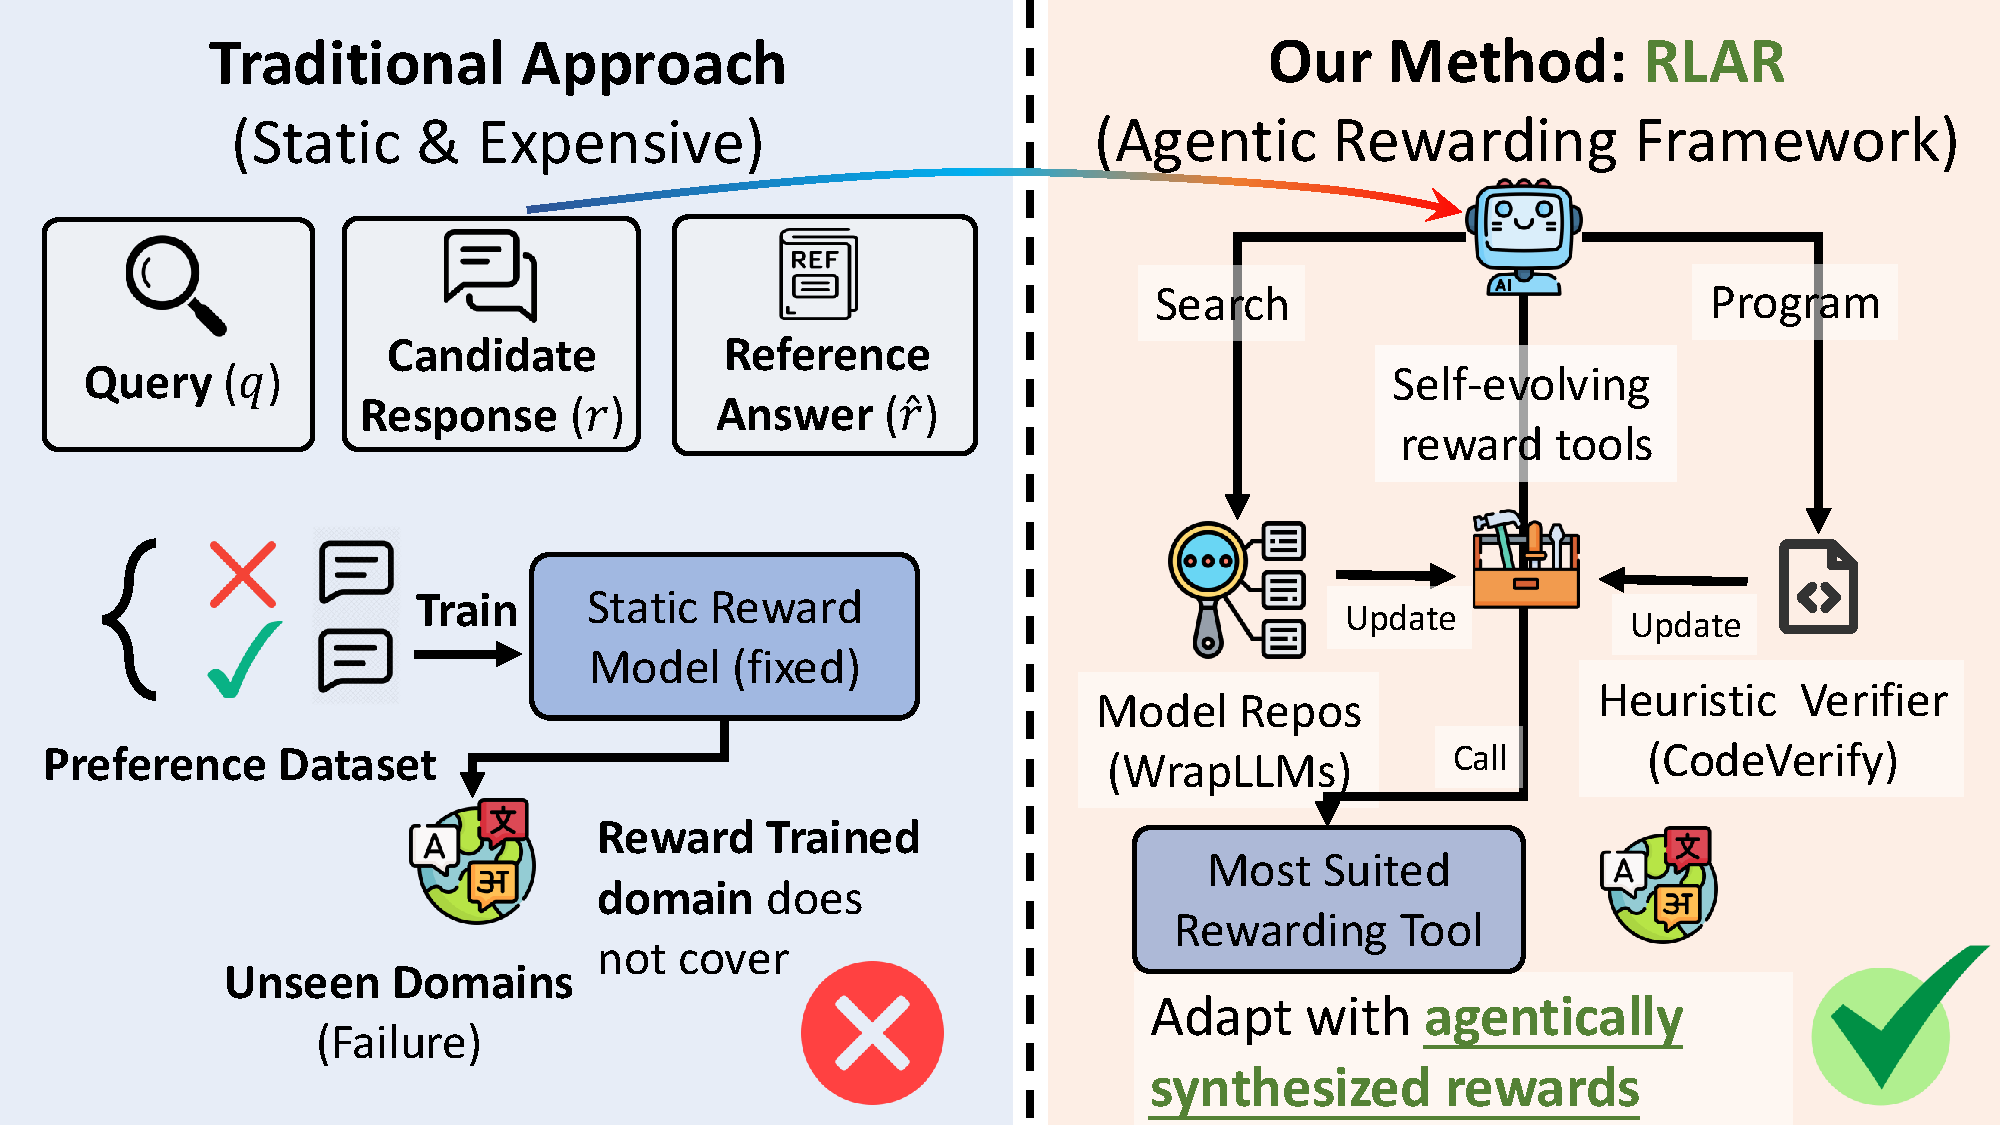
\includegraphics[width=0.95\linewidth]{Figures/intro_fig.pdf}
    \caption{A conceptual comparison between traditional reward modeling and our proposed RLAR framework.}
    \label{fig:intro_fig}
    \vspace{-4mm}
\end{wrapfigure}

To bridge this gap, we propose \textbf{\method{}} (Reinforcement Learning from Agentic Rewards), a self-evolving framework that \textbf{regards the reward functions as callable tools} and is easy to scale over heterogeneous query distributions.
\method{} primarily leverages LLMs' tool-calling capabilities to assign reward scores for the querying task sample based on existing tools. 
Once there are no suitable local tools, \method{} explores online model checkpoint repositories in search of matching neural models, as well as designs code-based executable functions for the current task. The runtime tool library evolves with the appended tools.
We calibrate the final reward output from \method{} with benchmarks such as \textsc{RewardBench-V2}~\citep{rewardbench2} before deploying it in online RL training.
By shifting from learning LLMs' ``\textbf{generated score reward}'' to ``\textbf{designed reward function}'', \method{} ensures high-fidelity rewards across distributions while significantly reducing the inference costs associated with constructing additional reward models.

We evaluate \method{} across a diverse suite of tasks, including math reasoning~\citep{hendrycks2021measuringmathematicalproblemsolving, gsm8k}, code~\citep{leetcodedataset, mbpp}, translation~\citep{benchmax, nllb2022, flores101, twoevaldatasets}, and general chat~\citep{ultrachat}.
We compare our agentic reward synthesis-leveraging framework against state-of-the-art static reward models, including classification~\citep{skyworkreward}, generative ones~\citep{skyworkcritic2024}, and GPT5-as-a-judge. 
\method{} achieves overall performance improvements of \(10.4\%\) and \(61.9\%\) on Llama-3.1-8B and Qwen3-8B, significantly surpassing static classification and generative baselines. 
Unlike baselines such as \textbf{SkyLlama}, which suffer from performance decrements in math reasoning tasks during mixed training, \method{} dynamically models domain objectives across math, code, translation, and chat. 
Notably, \method{} demonstrates enhanced robustness to \textbf{format and verbosity hacking}, whereas loopholes persist in baselines, including GPT5-as-a-judge.
Finally, compared to GPT-5-as-a-judge, \method{} reduces API token consumption by approximately \(80\%\) and GPU training hours by \(75\%\), demonstrating \method{}'s scaling potential.
Ablation studies reveal that each synthesis pathway serves a distinct role: \textbf{CodeVerify}-generated verifiers are critical for rule-heavy tasks (math, code), while \textbf{WrapLLM}-retrieved neural models are essential for open-ended tasks (chat, translation). Furthermore, replacing the agentic selector with random reward assignment degrades performance across nearly all benchmarks, confirming that \method{}'s gains stem from precise per-query reward routing, not merely from reward tool diversity.
The data and code are available on \url{https://anonymous.4open.science/r/NeurIPS2026-RLAR/}.


% Further experiments demonstrate that the effectiveness of RLAR mainly comes from the accurate reward tool selection, and we calibrate it with \textsc{RewardBench-v2}. Our \textbf{Agentic Reward Tool Selector} obtained \(90.44\%\) accuracy by routing queries to the most suitable reward models, outperforming both the SOTA \(87.19\%\) and SOTA-model logits ensembling \(87.44\%\). These results indicate that dynamic routing more effectively approaches the theoretical upper bound. 


\section{Preliminaries}

\subsection{Task Definition} \label{sec:task_definition}

We investigate the problem of reinforcement learning in LLM post-training stage for complex, mixed-domain text generation tasks. The core objective is to train a single policy model that achieves high performance across multiple task domains without sacrificing the quality of any individual task.
Let \(\{ D_1, D_2, \dots, D_n \}\) denote datasets from \(n\) different domains, each corresponding to one type of task (e.g., translation, summarization, question answering).  
We define a mixed-domain distribution \(D = \{ D_1, D_2, \dots, D_n \}\).
Our goal is to train a policy model \(A\) that maximizes expected performance over \(D\) under a multi-task reinforcement learning framework:  
\[
\max_{A} \; \mathbb{E}_{d \sim D} \left[ R(A(d)) \right],
\]  
where \(R(A(d))\) denotes the reward of policy inference on sample \(d\). The reward is computed from test-time metrics, such as success rate, accuracy, LLM-judge score, and other task-specific metrics. 
We study the blended domains where real LLM post-training usually focuses: \textbf{mathematical reasoning}, \textbf{code and programming}, \textbf{translation}, and \textbf{general conversation} tasks. We show information about the datasets used in our experiments in Table~\ref{tab:dataset_stat}.


\subsection{LLM post-training with online RL} \label{sec:rl_algo}


In reinforcement learning from human feedback (RLHF), the \textbf{Proximal Policy Optimization} algorithm~\citep{ppo} is frequently employed for policy optimization.  
The typical workflow begins with a \textit{warm-start training} phase in which a \textbf{Value Model} (often a reward model) is learned. Training triplets \((x, y_{+}, y_{-})\) are sampled from human preference data, with \(y_{+}\) being preferred over \(y_-\). Let \(r_{\theta}(x, y)\) be the reward assigned by the model given prompt \(x\) and response \(y\); the learning objective function can be expressed as:
\begin{equation*}
    \mathcal{L}(\theta) = -\frac{1}{N} \,\mathbb{E}_{(x,y_+, y_-) \sim D } \bigg[ \log \sigma \big( \Delta r_{\theta} \big) \bigg],
\end{equation*}
where \(\sigma(\cdot)\) is the logistic sigmoid function and \(\Delta r_{\theta} = r_{\theta}(x, y_+) - r_{\theta}(x, y_-)\)  .

We adopt a more training-efficient framework. The \textbf{Group Relative Policy Optimization} (GRPO)~\citep{grpo} modifies the advantage estimation to reduce the dependence on a learnable value model for estimating the advantage baseline. Instead, GRPO computes the normalized advantage within a group of sampled outputs \(\hat{A}_{i} = \frac{r_i - \mathrm{mean}(r)}{\mathrm{std}(r)}  \), 
where \(r=\{ r_i \}_{i=1}^G\) are the rewards assigned to \(G\) candidate outputs for the same prompt, \(\mathrm{mean}(r)\) and \(\mathrm{std}(r)\) are computed over the group. Also, the Kullback-Leibler Divergence term is removed from the per-step reward and is instead applied directly to the overall optimization objective:
\begin{align}
\max_{\phi} \; \;
& \mathbb{E}_{\substack{x \sim D, \\ \{y_i\}_{i=1}^G \sim \pi_{\mathrm{old}}(y_i|x)}} 
\Bigg[
   \frac{1}{G} \sum_{i=1}^G
   \min \Bigg\{
      \frac{\pi_{\theta}(y_i|x)}{\pi_{\mathrm{old}}(y_i|x)} ,  \;
      \nonumber \\[-0.5em]
& 
      \mathrm{clip}\!\left(
         \frac{\pi_{\theta}(y_i|x)}{\pi_{\mathrm{old}}(y_i|x)},
         1 - \epsilon, \;
         1 + \epsilon
      \right) 
   \Bigg\} \hat{A}_{i},
\Bigg] 
- \beta \, \mathbb{D}_{\mathrm{KL}}\!\left[ \pi_{\phi} \;\|\; \pi_{\mathrm{ref}} \right].
\end{align}

% % 插入一个表格，让读者一目了然
\begin{table}[t]
    \centering
    \caption{Summary of domains considered across Math, Code, Translation, and General Conversation.}
    \label{tab:dataset_stat}
    \small % Slightly smaller font to ensure fit if necessary
    \resizebox{0.8\textwidth}{!}{ %
    \begin{tabular}{llccccl}
    \toprule
    \textbf{Domain} & \textbf{Dataset} & \textbf{Train Size} & \textbf{Test Size} & \textbf{OOD} & \textbf{Evaluation Metric} \\
    \midrule
    \multirow{3}{*}{\textbf{Math}} 
        & \textsc{GSM8k}          & 1,500 & 1,319 & \xmark & \multirow{3}{*}{Numeric Match} \\
        & \textsc{Hendrycks-Math} & 1,500 & 500   & \xmark &  \\
        & \textsc{AIME-24/25}        & 0     & 60    & \cmark &  \\
    \midrule
    \multirow{2}{*}{\textbf{Code}} 
        & \textsc{LeetCode-Dataset}       & 2,585 & 223   & \xmark & \multirow{2}{*}{Unit Test Execution} \\
        & \textsc{MBPP}           & 0     & 974   & \cmark &  \\
    \midrule
    \multirow{2}{*}{\textbf{Translation}} 
        & \textsc{Flores-200}     & 3,000 & 300   & \xmark & \multirow{2}{*}{Hybrid (LLM-Judge + BLEU)} \\
        & \textsc{WMT-24}         & 0     & 500   & \cmark &  \\
    \midrule
    \textbf{General} 
        & \textsc{UltraChat}      & 2,500 & 200   & \xmark & Model-based (LLM-as-a-Judge) \\
    \bottomrule
    \end{tabular}
    }
    \vspace{-4mm}
\end{table}




% This formulation reduces sensitivity to reward model estimation errors by leveraging relative comparisons within output groups.




% \subsection{Task Design and Evaluation} \label{sec:task_design}







\section{Methodology}
\label{sec:method}

\method{} treats reward design as a bounded interaction with tools: an agent constructs an executable reward program, tests its behavior against task-provided evidence, and revises it before reuse. The output is a program and its validation record, rather than a score for one response. We distinguish \emph{construction tools}, which help the agent design and test a program, from \emph{scoring components}, which the resulting program invokes. A single controller coordinates construction; additional specialized agents are not required.

\noindent\textbf{Scope of this revision.} We specify a revised protocol for objectively verifiable tasks, initially mathematics and code. The construction-loop comparisons and Qwen3-8B distillation below are proposed evaluations, not completed experiments. Earlier selection and RL results do not establish their effectiveness; the selection-only study is retained in Appendix~\ref{apd:legacy_routing}. Extending validation to open-ended translation and dialogue requires independent quality labels and is outside this revision's primary scope.

\subsection{Reward Construction as a Task}
\label{sec:formulation}

A construction task $\tau$ provides a specification $d_\tau$, permitted scoring resources $\mathcal{A}_\tau$, and two disjoint test suites $V_\tau^{\mathrm{dev}}$ and $V_\tau^{\mathrm{audit}}$. The specification defines the objective, input schema, available references or execution tests, and any explicit output constraints, including their priority relative to content correctness. Each suite contains response examples, oracle-derived quality labels or comparisons, and valid transformations for checking reward behavior. These labels come from task verifiers fixed before construction, not from the reward designer's own judgments. Development tests provide feedback; the audit suite remains inaccessible until the submitted program is frozen.

The agent produces a reward artifact $g_\tau$ with interface
\begin{equation}
    g_\tau(q,r,\hat r,z) \longrightarrow (s,e),
    \qquad s\in[0,1],
\end{equation}
where $q$ is a query, $r$ a response, $\hat r$ an optional training reference, and $z$ the permitted task metadata or execution tests. The structured record $e$ contains component scores and execution status. Infrastructure failures return a distinct error status rather than a valid low score. An artifact comprises source code, an applicability description, pinned dependencies, and fixed score transformations and composition parameters. References and tests are function inputs; programs may not embed development-example identifiers or answer lookup tables.

The harness consumes a stream of query records and emits one construction result per processed record. Each result stores a serialized reward definition with function-source strings, or a key into an optional content-addressed library. A key hashes the complete definition, including composition and runtime dependencies; query inputs and validation evidence are stored separately. A query without an adequate test pack can yield an unvalidated definition, but not a claim of validated reward quality.

Construction occurs at the level of a task specification or reusable task subtype. At scoring time, a router selects an applicable artifact from the library using the query and permitted metadata. It does not inspect the current candidate responses to choose their reward function. When no artifact covers the required contract, a bounded construction episode is triggered using the task's development pack.

\subsection{Modular Tools and a Fixed Reward-Model Catalogue}
\label{sec:synthesis}

The stream interface requires only structured reward definitions, task-aware validation, and submission (Table~\ref{tab:construction_tools}). General file and shell operations are optional adapters for agents that benefit from a coding workspace. Task analysis is performed by the controller from the supplied task pack; model cards are ordinary read-only resources. Neither requires a separate LLM-backed tool. Existing coding-agent file and shell interfaces can be adapted to this schema. A dedicated registry search is optional for larger libraries; small catalogues can be read directly.

\begin{table}[t]
\centering
\caption{Minimal construction interface. File and shell tools are optional and scoped to permitted resources. Versioning, validation, and registration remain harness responsibilities.}
\label{tab:construction_tools}
\small
\begin{tabularx}{\linewidth}{@{}lXX@{}}
\toprule
\textbf{Tool} & \textbf{Input} & \textbf{Observation / effect} \\
\midrule
\texttt{read\_file} & Path and bounded line range. & Content, file hash, and truncation status. \\
\texttt{write\_file} & Path, content, expected prior hash. & Updated path and content hash. \\
\texttt{edit\_file} & Path, prior hash, exact replacement. & Change record and updated hash; conflicts are explicit. \\
\texttt{run\_command} & Command, working directory, timeout. & Exit code, bounded stdout/stderr, and termination reason. \\
\texttt{test\_reward} & Serialized definition, development profile, on-pass policy. & Version-bound report; optional finalization after full admission checks. \\
\texttt{submit\_reward} & Artifact ID and validation run ID. & Acceptance or rejection and selected artifact; the driver persists the result. \\
\bottomrule
\end{tabularx}
\end{table}

\noindent\textbf{Fixed neural scoring resources.} We replace online model search, checkpoint downloading, and automatic deployment with a small, preselected catalogue $\mathcal M_0$ of representative open-source reward models, exposed through a uniform \texttt{score\_model} API. Each entry includes its model card and a versioned inference contract. The catalogue is selected before evaluation, without using target audit results, and shared by all construction baselines. Exact checkpoints and revisions belong in the experiment manifest. Inspecting a card suggests applicability; it does not certify reward quality. The agent can use these models as components, combine them with rules, or omit them. Catalogue membership stays fixed even as the library of constructed programs grows.

\noindent\textbf{Single reward and checklist modes.} The run configuration selects a single function or a checklist. In checklist mode, the agent specifies a bounded list of criteria and a source-code string for each component; the plan and all implementations can share one completion. The entire list and its aggregation form one artifact. Functions may implement answer checks, code execution against permitted tests, or calls to model APIs. A fixed runtime aggregates their normalized scores:
\begin{equation}
    s = h_\tau(q,r,z)\frac{1}{|\mathcal V|}\sum_{j\in\mathcal V} c_j\!\left(f_j(q,r,\hat r,z)\right),
    \quad \mathcal V\neq\emptyset,
\end{equation}
Here $\mathcal V$ is the set of successfully executed components. Single mode uses one function; checklist mode uses the arithmetic mean over successful components, with a bounded planned count $m$. All-component execution failure returns no score and a failed status. Coverage $|\mathcal V|/m$ and each component's status accompany partial scores. This revision does not expose trainable or agent-selected weights. Each $c_j$ maps its component to $[0,1]$ with larger values indicating better quality. Component count is bounded, and normalization, criteria, and the component list are fixed before scoring a query's candidates. The planned list is fixed, and membership in $\mathcal V$ is determined only by the declared execution-status rule, never by dropping low scores. Valid zero scores remain in the mean. Partial execution does not itself establish reward quality. The optional gate $h_\tau\in\{0,1\}$ enforces requirements explicitly present in the task; it is $1$ when no hard gate is required. Duplicate or overlapping criteria are diagnosed because repeated checks can implicitly alter emphasis even under equal averaging. Both component behavior and the final aggregate require validation; a list of executable checks alone does not establish reward quality.

\subsection{A Bounded Construction and Repair Loop}
\label{sec:routing}

An episode starts from the current query/task pack, a library snapshot, and an explicit resource budget $B$; a writable workspace is optional. The controller inspects relevant contracts, retrieves reusable artifacts, writes or adapts a candidate, and calls \texttt{test\_reward}. The harness snapshots the entire artifact before testing and binds its report to that immutable version. A failed comparison or execution error can lead to a targeted source revision and another test. Submission checks the matching full-development report; agent-written logs cannot certify acceptance. The interaction is
\begin{equation}
    a_t\sim\pi_{\mathrm{design}}(\cdot\mid C_t),
    \qquad o_t=\operatorname{Tool}(a_t),
\end{equation}
where $C_t=P_{\mathrm{run}}\Vert P_\tau\Vert h_t$ is the logical message sequence and $\Vert$ denotes concatenation. The run prefix fixes instructions and tool schemas; the episode prefix fixes the task pack, initial library snapshot, mode, and initial budget. History appends complete assistant actions, their tool observations, and updated state, including remaining budget $B_t$. Earlier messages are never rewritten. Each episode has at most one controller request in flight; independent tools may run as a batch, with results appended in call order before the next decision. Different queries have separate histories. This preserves a common prefix and permits provider-supported prefix caching without assuming a cache hit.

\noindent\textbf{Reducing model requests.} The controller can emit a plan and complete definition in one call. Tools perform lookup, hashing, batched testing, and persistence without auxiliary LLM planners or judges. Under the predeclared on-pass submission policy, \texttt{test\_reward} invokes the same trusted finalizer as explicit submission after full admission checks, eliminating a confirmation-only model turn. Repairable failures trigger further decisions. Compatible validated reuse can require zero controller calls, and a new artifact that passes immediately can require one. These are execution paths, not measured speedups; retries and neural scoring requests are counted separately (Appendix~\ref{apd:llm_protocol}).

The budget limits controller tokens, candidate submissions, and test executions; their realized costs are reported separately. Finalization selects an eligible candidate or records failure when the budget is exhausted. A retained earlier candidate must pass the same development criteria. Failed episodes remain part of the evaluation denominator. Budgets cover all checklist items and retries jointly. A supervisor enforces call and episode deadlines, limits repeated invalid/no-progress actions, and never resets the full budget for each component. Context capacity is checked before requests; exhaustion follows the same termination rule rather than silently removing history or invoking an LLM summarizer.

The outer driver owns stream iteration and durable output. Record-specific failures produce explicit results and allow subsequent queries to proceed; authentication, output-storage, or persistent infrastructure failures stop the run. EOF, cancellation, and the global budget bound the outer loop. Committed results are resumed idempotently from input/configuration digests and the recorded library state. Source persistence, execution, and isolation are separate interfaces; Docker is not required (Appendix~\ref{apd:harness_isolation}).

\begin{figure}[t]
\centering
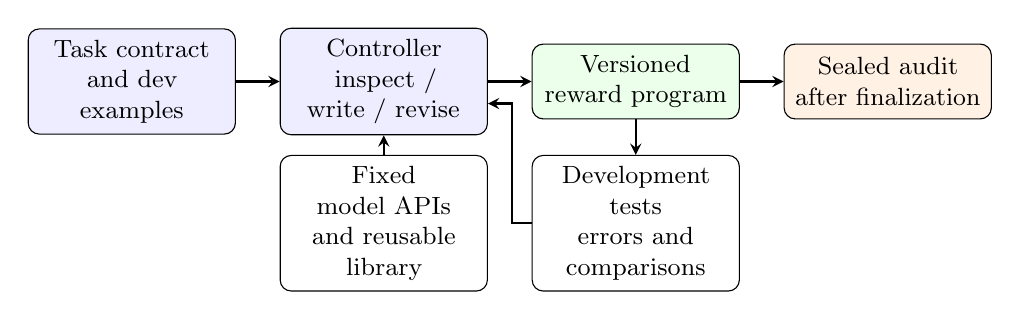
\begin{tikzpicture}[>=stealth, font=\small,
 box/.style={draw,rounded corners,align=center,text width=2.35cm,minimum height=0.95cm,inner sep=4pt},
 flow/.style={->,thick}]
\node[box,fill=blue!7] (task) at (0,0) {Task contract\\and dev examples};
\node[box,fill=blue!7] (agent) at (3.2,0) {Controller\\inspect / write / revise};
\node[box,fill=green!8] (program) at (6.4,0) {Versioned\\reward program};
\node[box,fill=orange!10] (audit) at (9.6,0) {Sealed audit\\after finalization};
\node[box] (library) at (3.2,-1.8) {Fixed model APIs\\and reusable library};
\node[box] (tests) at (6.4,-1.8) {Development tests\\errors and comparisons};
\draw[flow] (task) -- (agent);
\draw[flow] (agent) -- (program);
\draw[flow] (program) -- (audit);
\draw[flow] (library) -- (agent);
\draw[flow] (program) -- (tests);
\draw[flow] (tests.west) -- ++(-0.25,0) |- ([yshift=-0.28cm]agent.east);
\end{tikzpicture}
\caption{Revised construction loop. Development feedback supports repair; audit outcomes never return to the controller. Accepted artifacts accumulate in the library, while all interaction events are stored separately as traces.}
\label{fig:main_fig}
\end{figure}

This loop provides a testable hypothesis for agentic design: observed failures enable revisions that a single completion cannot condition on. Extra calls alone do not establish an advantage. We therefore compare against both a single completion and independent sampling under matched budgets (Section~\ref{sec:design_controls}).

\subsection{Testing the Reward Function Itself}
\label{sec:verification}

\noindent\textbf{Independent task evidence.} For mathematics, suite labels are derived from trusted answers and an independently implemented equivalence checker; for code, from trusted execution tests. The suites include correct and incorrect responses, parser edge cases, and oracle-validated perturbations. Content correctness and instruction compliance are evaluated separately. A proposed perturbation is admitted only if the task oracle confirms the intended relation; agent-generated tests are supplemental diagnostics, not a source of ground truth.

Let $P_\tau^v$ contain strictly ordered response pairs $(x^+,x^-)$ from suite $v$, where $x=(q,r,\hat r,z)$ and the task oracle prefers $x^+$ to $x^-$. Reward discrimination is
\begin{equation}
    Q_{\mathrm{rank}}^v(g)=\frac{1}{|P_\tau^v|}
       \sum_{(x^+,x^-)\in P_\tau^v}
       \mathbf{1}\{g_s(x^+)>g_s(x^-)\},
\end{equation}
where $g_s$ denotes the scalar output. Ties and execution failures do not pass a strict comparison. For pairs $E_\tau^v$ whose quality should be unchanged under the task contract, we also measure
\begin{equation}
    Q_{\mathrm{inv}}^v(g)=\frac{1}{|E_\tau^v|}
       \sum_{(x,x')\in E_\tau^v}
       \mathbf{1}\{|g_s(x)-g_s(x')|\leq\epsilon_\tau\}.
\end{equation}
The tolerance is fixed before comparison, and errors count as failures. Unchanged-quality examples may include equivalent numeric representations or permitted whitespace changes; strict comparisons include wrong-answer substitutions and confirmed code mutations. Constant rewards can pass invariance tests but fail discrimination, so neither metric is sufficient alone.

\noindent\textbf{Acceptance and audit.} We report a vector of execution success, ranking accuracy, invariance, constraint violations, and false acceptance/rejection rates at a development-fixed score threshold. Task-specific minimum coverage and acceptance thresholds are predefined on training/development tasks and shared by all methods. An artifact is registered only if its interface and required development criteria pass; this constitutes development validation, not proof of general correctness. The frozen final artifact is evaluated once on the sealed audit suite. Audit outcomes cannot guide repair, registration, or candidate selection. Split provenance, mutation families, and thresholds are detailed in Appendix~\ref{apd:construction_protocol}.

A strong objective verifier may already be an effective reward. Whenever it is available under the scoring contract, \emph{direct oracle reward} is a required baseline. We do not create an advantage by withholding an otherwise available checker from competing methods. Construction is useful only if it improves measurable quality, coverage, or cost over such direct use; downstream RL is needed to determine whether better offline diagnostics improve policy learning.

\subsection{Minimal Memory and Consistent RL Scoring}
\label{sec:library_memory}

The runtime retains only an episode workspace and a persistent artifact library $\mathcal F$. Each library entry stores code and version, applicability, dependencies, calibration, development-test provenance, and a short validation report. Tags and text matching suffice for retrieval. Equivalent source/configuration hashes are deduplicated, revisions receive new versions, and previously accepted artifacts are immutable. Raw transcripts remain in the trace store rather than becoming an additional long-term memory system. Evaluation splits cannot share test-derived artifacts.

For a query $q$, the router selects or constructs one artifact $g_q$ before scoring its rollout group $\{r_i\}_{i=1}^{G}$. All candidates use the same artifact version, scoring components, calibration, and equal-mean aggregation:
\begin{equation}
    s_i=g_{q,s}(q,r_i,\hat r,z),\qquad
    A_i=\frac{s_i-\bar s}{\operatorname{std}(s)+\epsilon_{\mathrm{adv}}}.
\end{equation}
Zero-variance groups receive zero advantages. Candidate-caused failures, such as invalid code or a candidate exceeding its execution limit, follow the task contract; infrastructure/API failures are logged separately. With partial execution, a candidate uses the mean of its successful components and records their mask. Different masks can affect group comparability; coverage and missingness patterns must therefore be evaluated separately. If all components fail for a candidate, its score is invalid and the downstream group follows a predeclared retry/fallback or omission policy, rather than treating failure as zero. Function updates take effect only for a subsequent rollout batch; rewards are not recomputed midway through optimization of an existing batch.

\subsection{Recorded Traces and Learning to Design Rewards}
\label{sec:trace_learning}

We record every observable construction event, including task and split IDs, the library snapshot, controller/model versions, tool arguments and results, source patches, test reports, finalization status, tokens, latency, and cost. Brief explicit design notes can be logged, but the trace does not depend on access to hidden model reasoning. Failures and repairs are retained, and versioned observations support replay. Audit records are stored separately and excluded from the controller history.

To test whether Qwen3-8B can learn this capability, a stronger teacher collects construction traces on training tasks. Successful development-validated traces, including their failed intermediate attempts and subsequent repairs, supply supervised targets for tool selection, arguments, code edits, and final submission. Training applies next-token loss only to assistant actions and program outputs; tool observations are conditioning context, not prediction targets. Task families/templates and their derived examples are split before trace collection and library construction. No held-out-task artifacts or audit feedback enter student training.

The student is evaluated as a reward designer with the same APIs, initial library, and budget as the teacher. It is distinct from any Qwen3-8B policy trained downstream using the resulting rewards. Comparisons include the untrained student, final-program-only SFT, full-trace SFT, and the teacher. Primary outcomes are held-out reward quality, successful construction rate, repair after observed failures, and construction cost, rather than imitation of the teacher's wording. This protocol tests learnability; no successful distillation result is assumed.

\subsection{Comparisons That Isolate Agentic Construction}
\label{sec:design_controls}

The primary baseline uses one chat completion to produce an executable reward artifact. It receives the same task pack, initial library, model cards, permitted scoring APIs, and labeled development examples as the agent; it receives no feedback from executing its own draft. Every submitted artifact is scored by the same external harness. We additionally compare budget-matched independent drafts selected by a fixed development evaluator, and multi-turn self-revision without execution observations. These separate adaptive use of feedback from increased sampling or generation budget.

Reward representation (single versus checklist) is crossed with construction strategy; checklist component evaluations count toward the same total budget. Module ablations remove execution feedback, persistent-library reuse, custom code construction, or neural scoring APIs one at a time. The no-execution-feedback condition also disables construction-time Bash and interactive scoring calls; removing only \texttt{test\_reward} measures the value of standardized validation while leaving self-written execution feedback available. Fixed versus accumulating libraries are compared on identically ordered construction streams with separate, uncontaminated audit sets. All variants use the same resource accounting, failure handling, and final evaluation. We report per-task metrics and quality--cost tradeoffs; any superiority over single-turn design is an empirical question. Appendix~\ref{apd:construction_protocol} specifies the controls and trace protocol.


\section{Experiments}

\noindent\textbf{Revision status.} The results in this section are retained from the earlier RLAR implementation. They have not been rerun with the construction, validation, and group-scoring protocol in Section~\ref{sec:method}. The revised primary evaluation concerns objectively verifiable mathematics and code tasks; historical translation/dialogue results are not evidence for the new validation protocol.

% We evaluate \method{} in two stages. First, we validate the core reward routing and selection mechanism on \textsc{RewardBench-v2} to confirm the inherent correctness of the agentic reward design (\S\ref{sec:eval_routing}). Then, we deploy \method{} in full RL post-training across four diverse task domains to assess its end-to-end effectiveness.


\subsection{Dataset and Evaluation}

We conduct RL training and evaluation across four representative task domains, each chosen to stress-test different aspects of the reward system. \textbf{Math Reasoning:} We use \textsc{GSM8k}~\citep{gsm8k} and \textsc{Hendrycks-MATH}~\citep{hendrycks2021measuringmathematicalproblemsolving} for mathematical reasoning. The goal is to reason toward the final numeric solution. \textbf{Coding:} We select the \textsc{LeetCode-Dataset}~\citep{leetcodedataset}, which requires the model to fill in LeetCode cloze-style function implementations. \textbf{Translation:} We sample from \textsc{FLORES-101}~\citep{flores101} to cover 20 translation pairs across five languages (CN, DE, EN, FR, JP). This task requires mastery across languages and is important for LLMs' accessibility to worldwide users, especially non-English speakers. \textbf{General Alignment:} \textsc{UltraChat}~\citep{ultrachat} is employed to train and evaluate multi-turn dialogue and instruction-following capabilities.


\noindent\textbf{Generalization Challenge.}\quad To assess the robustness of the trained policy, we include benchmarks such as \textsc{AIME-24/25} for math reasoning, \textsc{MBPP}~\citep{mbpp} for Python synthesis, and \textsc{WMT-24} for unseen translation contexts. 
These benchmarks evaluate whether the post-trained model can generalize rather than overfit to the specific heuristics of the training reward models, as an indication of reward hacking.



\noindent\textbf{Data Processing.} For all training queries, we apply an automated filtering process, requiring an LLM to discard samples with low query or response quality. The prompt is provided in Appendix~\ref{apd:prompt_for_data_filter}. We then uniformly downsample over \textsc{GSM8k, Hendrycks-Math, Flores-200, WMT-24, Ultra-Chat} to ensure a balanced distribution of queries across different dataset sources. To facilitate our experiments, we obtain the reasoning outputs of \textsc{GPT-5} on all queries. For dataset queries lacking human-annotated reasoning references, we supplement them with the results from \textsc{GPT-5}. Table~\ref{tab:dataset_stat} shows the statistics of the train and validation sets. A more detailed introduction of the tasks and our selected datasets is provided in Appendix~\ref{apd:data}.



\noindent\textbf{Evaluation Metrics.} To ensure evaluation rigor, we apply Numeric Exact Match (\textbf{NEM}) at Best@1 for mathematical reasoning tasks. For code generation, we report \textbf{pass@1} verified by automated code executors.
For translation tasks, we report both \textbf{BLEU}~\citep{papineni-etal-2002-bleu} and \textbf{LLM-judge} scores, while general dialogue tasks are evaluated solely by the LLM-judge. Additionally, we measure the \textbf{average generation lengths} across all benchmarks to detect potential reward-hacking behaviors associated with the verbosity bias inherent in LLM-based rewarding. GPT-5 is utilized as the primary evaluator for all LLM-as-a-judge assessments, and the 0-10 scoring range is normalized to 0-100 in accordance with other metrics.
We provide an \textbf{average score} across all benchmarks, where the translation score is a composite of 0.5 BLEU-2 and 0.5 LLM-judge.



% ---------------------------------------------------------
% Table 1: Math and Code Reasoning
% ---------------------------------------------------------
\begin{table*}[t]
    \centering
    % \caption{\textbf{Main Experiment Results (Math \& Code)}. For each testset, \textbf{Bold} indicates the best result under that metric, and \underline{underline} indicates the second best within each model group. \up{Increment} and \down{decrement} are calculated relative to the Zero-Shot baseline for Llama and Qwen. \textbf{NEM} shorts for numeric exact match, \textbf{HEND} shorts for \textsc{Hendrycks-Math}, and \textbf{LCode} shorts for \textsc{LeetCode-Dataset}. The bold benchmarks (\textbf{AIME24/25, MBPP}) indicate that they do not include the training data.}
    \caption{\textbf{Main Results (Math \& Code)}. \textbf{Bold}/\underline{underline}: best/second-best. \up/\down: changes vs. Zero-Shot baselines. \textbf{NEM}: Numeric Exact Match. \textsc{HEND}: \textsc{Hendrycks-Math}. \textsc{LCode}: \textsc{LeetCode}. \textbf{Bold} datasets denote unseen training data. \textbf{Avg.}: overall average across all four task domains (shared with Table~\ref{tab:main_res_language}). \textbf{M\&C}: local average over Math \& Code benchmarks in this table only.}
    \label{tab:main_res_math_code}
    \resizebox{0.85\textwidth}{!}{%
    \begin{tabular}{l cc cccc cc}
    \toprule
    \textbf{Domain} & \textbf{Avg.} & \textbf{M\&C} & \multicolumn{4}{c}{\textbf{Math}} & \multicolumn{2}{c}{\textbf{Code}} \\
    \cmidrule(r){1-1} \cmidrule(r){2-2} \cmidrule(r){3-3} \cmidrule(r){4-7} \cmidrule(r){8-9}
    \textbf{Dataset} & \textbf{Score} & \textbf{Avg.} & GSM8k & HEND & \textbf{AIME24} & \textbf{AIME25} & LCode & \textbf{MBPP} \\ \midrule
    \textbf{Metric} & - & - & NEM & Pass@k & NEM & NEM & Pass@k & Pass@k \\
    \midrule
    \multicolumn{9}{c}{\cellcolor{lightgreen}{\textit{\textbf{Llama-3.1-8B}}}} \\ \midrule
    Base & 37.81 & 28.23 & 60.50 & 49.80 & 6.67 & 0.00 & \underline{11.21} & 41.17 \\
    SkyLlama & 23.47 & 13.17 & 11.30 \down{49.20} & 47.60 \down{2.20} & 3.33 \down{3.34} & 0.00 \neut{-} & 8.97 \down{2.24} & 7.80 \down{33.37} \\
    SeedX & 17.29 & 10.64 & 1.21 \down{59.29} & 42.20 \down{7.60} & 6.67 \neut{-} & 0.00 \neut{-} & 0.00 \down{11.21} & 13.76 \down{27.41} \\
    SkyQwen & 31.68 & 18.96 & 16.15 \down{44.35} & 46.60 \down{3.20} & 3.33 \down{3.34} & 0.00 \neut{-} & \textbf{11.66 \up{0.45}} & 36.04 \down{5.13} \\
    SkyCritic & 34.05 & 26.43 & 44.58 \down{15.92} & 48.00 \down{1.80} & \underline{10.00 \up{3.33}} & 0.00 \neut{-} & 10.31 \down{0.90} & \textbf{45.69 \up{4.52}} \\
    GPT5-Judge & \underline{39.89} & \underline{30.14} & \underline{71.95 \up{11.45}} & 43.20 \down{6.60} & 6.67 \neut{-} & \underline{6.67 \up{6.67}} & 7.17 \down{4.04} & \underline{45.17 \up{4.00}} \\
    Human & 33.56 & 22.79 & 42.38 \down{18.12} & 40.00 \down{9.80} & 3.33 \down{3.34} & 3.33 \up{3.33} & 10.31 \down{0.90} & 37.37 \down{3.80} \\
    \textbf{RLAR}\small{(Ours)} & \textbf{41.73} & \textbf{33.84} & \textbf{73.61 \up{13.11}} & \textbf{54.60 \up{4.80}} & \textbf{13.33 \up{6.66}} & \textbf{6.67 \up{6.67}} & \textbf{11.66 \up{0.45}} & 43.18 \up{2.01} \\
    \midrule
    \multicolumn{9}{c}{\cellcolor{lightgreen}{\textit{\textbf{Qwen3-8B}}}} \\ \midrule
    Base & 29.12 & 12.61 & 31.99 & 19.80 & 3.33 & 0.00 & 6.28 & 14.27 \\
    SkyLlama & 29.25 & 12.49 & 0.00 \down{31.99} & 35.80 \up{16.00} & 10.00 \up{6.67} & 6.67 \up{6.67} & 7.62 \up{1.34} & 14.85 \up{0.58} \\
    SeedX & 35.14 & 21.26 & 0.00 \down{31.99} & \textbf{72.60 \up{52.80}} & 6.67 \up{3.34} & 6.67 \up{6.67} & 21.08 \up{14.80} & 20.53 \up{6.26} \\
    SkyQwen & 33.48 & 18.44 & 0.00 \down{31.99} & 67.00 \up{47.20} & 3.33 \neut{-} & 3.33 \up{3.33} & 15.70 \up{9.42} & \underline{21.25 \up{6.98}} \\
    SkyCritic & 39.07 & 26.95 & 51.71 \up{19.72} & 58.00 \up{38.20} & \textbf{20.00 \up{16.67}} & 6.67 \up{6.67} & 13.00 \up{6.72} & 12.32 \down{1.95} \\
    GPT5-Judge & \underline{45.85} & \underline{35.75} & \underline{91.96 \up{59.97}} & 56.20 \up{36.40} & 16.67 \up{13.34} & \underline{10.00 \up{10.00}} & \underline{21.52 \up{15.24}} & 18.17 \up{3.90} \\
    Human & 44.40 & 34.42 & \textbf{95.30 \up{63.31}} & 53.80 \up{34.00} & \textbf{20.00 \up{16.67}} & \underline{10.00 \up{10.00}} & 8.52 \up{2.24} & 18.89 \up{4.62} \\
    \textbf{RLAR}\small{(Ours)}  & \textbf{47.16} & \textbf{38.24} & 93.70 \up{61.71} & \underline{59.80 \up{40.00}} & \textbf{20.00 \up{16.67}} & \textbf{13.33 \up{13.33}} & \textbf{23.31 \up{17.03}} & 19.30 \up{5.03} \\
    \bottomrule
    \end{tabular}
    }
\end{table*}

% ---------------------------------------------------------
% Table 2: Translation, General Alignment, and Generation Length
% ---------------------------------------------------------
\begin{table*}[t]
    \centering
    % \caption{\textbf{Main Experiment Results (Translation, General \& Generation Stats)}. \up{Increment} and \down{decrement} are calculated relative to the Zero-Shot baseline for Llama and Qwen. \textbf{LLM-J} is short for LLM-judge, and \textbf{UChat} shorts for \textsc{Ultra-Chat}. The bold benchmark (\textbf{WMT24}) indicates that it does not include the training data.}
    \caption{\textbf{Main Results (Translation, General \& Stats)}. \textbf{Bold}/\underline{underline}: best/second-best. \up/\down: changes vs. Zero-Shot baselines. \textbf{LLM-J}: LLM-judge. \textbf{UChat}: \textsc{UltraChat}. The \textbf{bold} dataset (\textbf{WMT24}) is unseen during training. \textbf{Avg.}: overall average across all four task domains (shared with Table~\ref{tab:main_res_math_code}). \textbf{T\&G}: local average over Translation \& General benchmarks in this table only.}
    \label{tab:main_res_language}
    \resizebox{0.85\textwidth}{!}{%
    \begin{tabular}{l cc cccc cc}
    \toprule
    \textbf{Domain} & \textbf{Avg.} & \textbf{T\&G} & \multicolumn{4}{c}{\textbf{Translation}} & \textbf{General} & \textbf{Stats} \\
    \cmidrule(r){1-1} \cmidrule(r){2-2} \cmidrule(r){3-3} \cmidrule(r){4-7} \cmidrule(r){8-8} \cmidrule(r){9-9}
    \textbf{Dataset} & \textbf{Score} & \textbf{Avg.} & \multicolumn{2}{c}{Flore} & \multicolumn{2}{c}{\textbf{WMT24}} & UChat & Avg Len \\ \midrule
    \textbf{Metric} & - & - & BLEU-2 & LLM-J & BLEU-2 & LLM-J & LLM-J & \# \\
    \midrule
    \multicolumn{9}{c}{\cellcolor{lightgreen}{\textit{\textbf{Llama-3.1-8B}}}} \\ \midrule
    Base & 37.81 & 54.58 & 21.04 & 77.27 & 26.39 & 79.24 & \underline{68.97} & 152.84 \\
    SkyLlama & 23.47 & 40.88 & 21.16 \up{0.12} & 45.32 \down{31.95} & 23.23 \down{3.16} & 54.68 \down{24.56} & 60.03 \down{8.94} & 147.39 \\
    SeedX & 17.29 & 24.95 & 0.00 \down{21.04} & 23.24 \down{54.03} & 0.00 \down{26.39} & 42.76 \down{36.48} & 58.73 \down{10.24} & 89.95 \\
    SkyQwen & 31.68 & 55.52 & 26.42 \up{5.38} & 77.53 \up{0.26} & \underline{29.80 \up{3.41}} & 78.74 \down{0.50} & 65.13 \down{3.84} & 134.21 \\
    SkyCritic & 34.05 & 45.96 & 25.31 \up{4.27} & 42.53 \down{34.74} & 28.21 \up{1.82} & 67.82 \down{11.42} & 65.93 \down{3.04} & 106.97 \\
    GPT5-Judge & \underline{39.89} & \textbf{56.99} & 20.35 \down{0.69} & \textbf{82.50 \up{5.23}} & 26.37 \down{0.02} & \textbf{84.42 \up{5.18}} & \textbf{71.32 \up{2.35}} & 203.31 \\
    Human & 33.56 & 53.37 & \underline{26.61 \up{5.57}} & 70.67 \down{6.60} & \textbf{29.81 \up{3.42}} & 75.88 \down{3.36} & 63.87 \down{5.10} & 76.76 \\
    \textbf{RLAR}\small{(Ours)} & \textbf{41.73} & \underline{55.59} & \textbf{26.73 \up{5.69}} & \underline{74.83 \down{2.44}} & \underline{29.80 \up{3.41}} & \underline{79.54 \up{0.30}} & 67.03 \down{1.94} & 141.85 \\
    \midrule
    \multicolumn{9}{c}{\cellcolor{lightgreen}{\textit{\textbf{Qwen3-8B}}}} \\ \midrule
    Base & 29.12 & 60.22 & 28.46 & 84.00 & 32.50 & 84.46 & 71.70 & 1064.04 \\
    SkyLlama & 29.25 & 61.13 & 28.78 \up{0.32} & 85.59 \up{1.59} & 33.75 \up{1.25} & 86.54 \up{2.08} & 71.00 \down{0.70} & 844.96 \\
    SeedX & 35.14 & 61.31 & 30.34 \up{1.88} & 84.97 \up{0.97} & 35.25 \up{2.75} & 85.14 \up{0.68} & 70.83 \down{0.87} & 1135.82 \\
    SkyQwen & 33.48 & 61.58 & 29.70 \up{1.24} & 85.72 \up{1.72} & 33.82 \up{1.32} & 85.18 \up{0.72} & 73.47 \up{1.77} & 1192.12 \\
    SkyCritic & 39.07 & 61.37 & 28.66 \up{0.20} & 86.09 \up{2.09} & 32.52 \up{0.02} & 86.46 \up{2.00} & 73.10 \up{1.40} & 691.97 \\
    GPT5-Judge & \underline{45.85} & \textbf{63.59} & 28.31 \down{0.15} & \textbf{89.77 \up{5.77}} & 32.64 \up{0.14} & \textbf{88.93 \up{4.47}} & \textbf{78.32 \up{6.62}} & 1462.29 \\
    Human & 44.40 & \underline{62.32} & \underline{30.71 \up{2.25}} & 85.11 \up{1.11} & \underline{35.91 \up{3.41}} & 85.22 \up{0.76} & 74.63 \up{2.93} & 692.71 \\
    \textbf{RLAR}\small{(Ours)}  & \textbf{47.16} & 63.03 & \textbf{31.12 \up{2.66}} & \underline{86.49 \up{2.49}} & \textbf{36.07 \up{3.57}} & \underline{86.67 \up{2.21}} & \underline{74.81 \up{3.11}} & 986.23 \\
    \bottomrule
    \end{tabular}
    }
\end{table*}


% \begin{table*}[t]
%     \centering
%     \caption{\textbf{Main Experiment Results}. For each testset, \textbf{Bold} indicates the best result under that metric, and \underline{underline} indicates the second best within each model group. \up{Increment} and \down{decrement} are calculated relative to the Zero-Shot baseline for Llama and Qwen. \textbf{LLM-J} is short for LLM-judge, and \textbf{NEM} shorts for numeric exact match. \textbf{HEND} shorts for \textsc{Hendrycks-Math}, \textbf{LCode} shorts for \textsc{LeetCode-Dataset}, \textbf{UChat} shorts for \textsc{Ultra-Chat}. The bold benchmarks (\textbf{AIME24/25, MBPP, WMT24}) indicate that they do not include the training data.}
%     \label{tab:main_res}
%     \resizebox{\textwidth}{!}{%
%     \begin{tabular}{l c ccccc cccc ccc}
%     \toprule
%     \textbf{Domain} & \textbf{Avg.} & \multicolumn{4}{c}{\textbf{Math}} & \multicolumn{2}{c}{\textbf{Code}} & \multicolumn{4}{c}{\textbf{Translation}} & \multicolumn{2}{c}{\textbf{General}} \\
%     \cmidrule(r){1-1} \cmidrule(r){3-6} \cmidrule(r){7-8} \cmidrule(r){9-12} \cmidrule(r){13-14}
%     \textbf{Dataset} & \textbf{Score} & GSM8k & HEND & \textbf{AIME24} & \textbf{AIME25} & LCode & \textbf{MBPP} & \multicolumn{2}{c}{Flore} & \multicolumn{2}{c}{\textbf{WMT24}} & UChat & Avg Len \\ \midrule
%     \textbf{Metric} & - & NEM & Pass@k & NEM & NEM & Pass@k & Pass@k & BLEU-2 & LLM-J & BLEU-2 & LLM-J & LLM-J & \# \\
%     \midrule
%     \multicolumn{14}{c}{\cellcolor{lightgreen}{\textit{\textbf{Llama-3.1-8B}}}} \\ \midrule
%     Base & 37.81 & 60.50 & 49.80 & 6.67 & 0.00 & \underline{11.21} & 41.17 & 21.04 & 77.27 & 26.39 & 79.24 & \underline{68.97} & 152.84 \\
%     SkyLlama & 23.47 & 11.30 \down{49.20} & 47.60 \down{2.20} & 3.33 \down{3.34} & 0.00 \neut{-} & 8.97 \down{2.24} & 7.80 \down{33.37} & 21.16 \up{0.12} & 45.32 \down{31.95} & 23.23 \down{3.16} & 54.68 \down{24.56} & 60.03 \down{8.94} & 147.39 \\
%     SeedX & 17.29 & 1.21 \down{59.29} & 42.20 \down{7.60} & 6.67 \neut{-} & 0.00 \neut{-} & 0.00 \down{11.21} & 13.76 \down{27.41} & 0.00 \down{21.04} & 23.24 \down{54.03} & 0.00 \down{26.39} & 42.76 \down{36.48} & 58.73 \down{10.24} & 89.95 \\ 
%     SkyQwen & 31.68 & 16.15 \down{44.35} & 46.60 \down{3.20} & 3.33 \down{3.34} & 0.00 \neut{-} & \textbf{11.66 \up{0.45}} & 36.04 \down{5.13} & 26.42 \up{5.38} & 77.53 \up{0.26} & \underline{29.80 \up{3.41}} & 78.74 \down{0.50} & 65.13 \down{3.84} & 134.21 \\ 
%     SkyCritic & 34.05 & 44.58 \down{15.92} & 48.00 \down{1.80} & \underline{10.00 \up{3.33}} & 0.00 \neut{-} & 10.31 \down{0.90} & \textbf{45.69 \up{4.52}} & 25.31 \up{4.27} & 42.53 \down{34.74} & 28.21 \up{1.82} & 67.82 \down{11.42} & 65.93 \down{3.04} & 106.97 \\ 
%     GPT5-Judge & \underline{39.89} & \underline{71.95 \up{11.45}} & 43.20 \down{6.60} & 6.67 \neut{-} & \underline{6.67 \up{6.67}} & 7.17 \down{4.04} & \underline{45.17 \up{4.00}} & 20.35 \down{0.69} & \textbf{82.50 \up{5.23}} & 26.37 \down{0.02} & \textbf{84.42 \up{5.18}} & \textbf{71.32 \up{2.35}} & 203.31 \\ 
%     Human & 33.56 & 42.38 \down{18.12} & 40.00 \down{9.80} & 3.33 \down{3.34} & 3.33 \up{3.33} & 10.31 \down{0.90} & 37.37 \down{3.80} & \underline{26.61 \up{5.57}} & 70.67 \down{6.60} & \textbf{29.81 \up{3.42}} & 75.88 \down{3.36} & 63.87 \down{5.10} & 76.76 \\
%     \textbf{RLAR}\small{(Ours)} & \textbf{41.73} & \textbf{73.61 \up{13.11}} & \textbf{54.60 \up{4.80}} & \textbf{13.33 \up{6.66}} & \textbf{6.67 \up{6.67}} & \textbf{11.66 \up{0.45}} & 43.18 \up{2.01} & \textbf{26.73 \up{5.69}} & \underline{74.83 \down{2.44}} & \underline{29.80 \up{3.41}} & \underline{79.54 \up{0.30}} & 67.03 \down{1.94} & 141.85 \\
%     \midrule
%     \multicolumn{14}{c}{\cellcolor{lightgreen}{\textit{\textbf{Qwen3-8B}}}} \\ \midrule
%     Base & 29.12 & 31.99 & 19.80 & 3.33 & 0.00 & 6.28 & 14.27 & 28.46 & 84.00 & 32.50 & 84.46 & 71.70 & 1064.04 \\
%     SkyLlama & 29.25 & 0.00 \down{31.99} & 35.80 \up{16.00} & 10.00 \up{6.67} & 6.67 \up{6.67} & 7.62 \up{1.34} & 14.85 \up{0.58} & 28.78 \up{0.32} & 85.59 \up{1.59} & 33.75 \up{1.25} & 86.54 \up{2.08} & 71.00 \down{0.70} & 844.96 \\
%     SeedX & 35.14 & 0.00 \down{31.99} & \textbf{72.60 \up{52.80}} & 6.67 \up{3.34} & 6.67 \up{6.67} & 21.08 \up{14.80} & 20.53 \up{6.26} & 30.34 \up{1.88} & 84.97 \up{0.97} & 35.25 \up{2.75} & 85.14 \up{0.68} & 70.83 \down{0.87} & 1135.82 \\
%     SkyQwen & 33.48 & 0.00 \down{31.99} & 67.00 \up{47.20} & 3.33 \neut{-} & 3.33 \up{3.33} & 15.70 \up{9.42} & \underline{21.25 \up{6.98}} & 29.70 \up{1.24} & 85.72 \up{1.72} & 33.82 \up{1.32} & 85.18 \up{0.72} & 73.47 \up{1.77} & 1192.12 \\ 
%     SkyCritic & 39.07 & 51.71 \up{19.72} & 58.00 \up{38.20} & \textbf{20.00 \up{16.67}} & 6.67 \up{6.67} & 13.00 \up{6.72} & 12.32 \down{1.95} & 28.66 \up{0.20} & 86.09 \up{2.09} & 32.52 \up{0.02} & 86.46 \up{2.00} & 73.10 \up{1.40} & 691.97 \\
%     GPT5-Judge & \underline{45.85} & \underline{91.96 \up{59.97}} & 56.20 \up{36.40} & 16.67 \up{13.34} & \underline{10.00 \up{10.00}} & \underline{21.52 \up{15.24}} & 18.17 \up{3.90} & 28.31 \down{0.15} & \textbf{89.77 \up{5.77}} & 32.64 \up{0.14} & \textbf{88.93 \up{4.47}} & \textbf{78.32 \up{6.62}} & 1462.29 \\
%     Human & 44.40 & \textbf{95.30 \up{63.31}} & 53.80 \up{34.00} & \textbf{20.00 \up{16.67}} & \underline{10.00 \up{10.00}} & 8.52 \up{2.24} & 18.89 \up{4.62} & \underline{30.71 \up{2.25}} & 85.11 \up{1.11} & \underline{35.91 \up{3.41}} & 85.22 \up{0.76} & 74.63 \up{2.93} & 692.71 \\ 
%     \textbf{RLAR}\small{(Ours)}  & \textbf{47.16} & 93.70 \up{61.71} & \underline{59.80 \up{40.00}} & \textbf{20.00 \up{16.67}} & \textbf{13.33 \up{13.33}} & \textbf{23.31 \up{17.03}} & 19.30 \up{5.03} & \textbf{31.12 \up{2.66}} & \underline{86.49 \up{2.49}} & \textbf{36.07 \up{3.57}} & \underline{86.67 \up{2.21}} & \underline{74.81 \up{3.11}} & 986.23 \\
%     \bottomrule
%     \end{tabular}}
% \end{table*}


\subsection{Experimental Setup} \label{sec:experimental_setup}

\textbf{Base Models}: We use Qwen3-8B \citep{qwen3report} and Llama-3.1-8B-Instruct \citep{llama3report}. To examine various reward system architectures, we incorporate the following baselines:

\noindent\textbf{Classification Reward Baselines:} For the single classification reward model setting, we select \texttt{Skywork-Reward-V2-Llama-3.1-8B} (\textbf{SkyLlama}) and \texttt{Skywork-Reward-V2-Qwen3-8B} (\textbf{SkyQwen}) \citep{skyworkreward}, both of which represent the state-of-the-art on \textsc{RewardBench-v1/v2}~\citep{rewardbench, rewardbench2}. Additionally, we incorporate \texttt{Seed-X-8B-RM} (\textbf{SeedX}) due to its robust performance in multilingual contexts~\citep{seedX}.

\noindent\textbf{Generative Reward Baselines}: We evaluate \texttt{Skywork/Skywork-Critic-Llama-3.1-8B} (\textbf{SkyCritic})~\citep{skyworkcritic2024}, which generates natural language justifications with its judgments. Furthermore, we employ GPT-5-as-a-judge (\textbf{GPT5-judge}) as a high-capacity competitor, following the RL from AI Feedback paradigm~\citep{lee2024rlaif}. In this setup, GPT-5 is prompted to act as an evaluator, and its numerical scores are extracted as reward signals. The specific prompt template is detailed in Appendix~\ref{apd:judge_prompt}.

\noindent\textbf{Human Baseline:}
We implement a task-specific reward system to calibrate performance against optimal human-defined heuristics. For each task, the reward function is defined by the metrics most appropriate for the domain. Specifically, we utilize \textbf{NEM} for mathematics:
\[
    R_{\text{math}}(r, \hat{a}) =  \begin{cases}  1, & \text{if } \text{NEM}(r, \hat{a}) \\  0, & \text{otherwise} \end{cases}
\]
where $\hat{a}$ denotes the ground-truth numerical answer,
and \textbf{pass@1} for coding:
\[
R_{\text{code}}(r) =  \begin{cases}  1, & \text{if } \text{Exec}(r) = \text{Pass} \\  0, & \text{otherwise} \end{cases}
\]
For translation, the reward is calculated as a hybrid score \(w_1 \cdot \mathrm{BLEU} + w_2 \cdot \mathrm{SeedX} \), where the scaling factor is $w_1 = 1/2, w_2 = 1/2$ and SeedX's score is normalized to \((0, 1)\). The dialogue tasks are rewarded only by \textbf{SkyLlama}. We provide the \textbf{training configurations} in Appendix~\ref{sec:training_config} and \textbf{hyperparameters} for training in Appendix~\ref{apd:training_details}. \method{} is powered by GPT-5 by default.


\subsection{Main Results}

\noindent\textbf{Superiority of RLAR across Mixed Domains.} \quad
RLAR consistently outperforms both classification-based and generative reward baselines across multiple tasks and backbones (average score \(+10.4\%\) on Llama and \(+61.9\%\) on Qwen). 
Notably, RLAR achieves the best results on most benchmarks ($73.6$ NEM on GSM8k for Llama-3.1 and $23.3$ Pass@1 on LeetCode for Qwen3) without significant degradation in other distributions.
Improvements are also observed on the OOD benchmarks: \textsc{AIME-24}(\(+16.6\)), \textsc{AIME-25}(\(+13.3\)), \textsc{MBPP}(\(+5.03\)), and \textsc{WMT-24}(\(+3.41\) BLEU).
In contrast, \textbf{SkyLlama}, \textbf{SkyQwen}, and \textbf{SeedX} fail catastrophically with Qwen3 on \textsc{GSM-8k} (\(-31.9\)) and \textsc{UltraChat} while benefiting \textsc{Hendrycks} and \textsc{LeetCode}. This indicates that \method{} maintains stable and generalizable performance by dynamically modeling domain objectives into new reward designs without neglecting specific distributions.


On Llama-3.1, RL post-training shows limited headroom due to near-saturated base performance ($60.5$ on GSM8k, $41.17$ on MBPP). Nevertheless, \method{} yields the largest gains on most benchmarks ($+13.1$ on GSM-8k, $+3.41$ on \textsc{WMT} BLEU). \textbf{SkyLlama}, \textbf{SkyQwen}, and \textbf{SkyCritic} largely fail on GSM8k (\(-49.2, -44.3, -15.9\)) and rarely show benefits on OOD benchmarks.
\textbf{GPT5-Judge} improved Llama on \textsc{GSM8k} by \(11.4\) but degraded \textsc{Hendrycks-Math} by \(6.60\) and \textsc{LeetCode} by \(4.04\), demonstrating \method{}'s more robust reward design.



\noindent\textbf{Comparison with GPT5-Judge and Human Baseline.} \quad
While \textbf{GPT5-judge} is competitive, it exhibits vulnerabilities in rule-heavy tasks: on Llama-3.1, it triggers drops on Hendrycks-Math and LeetCode (-6.60/-4.04) while RLAR does not (+4.80/+0.45), suggesting reward systems lacking explicit rule verification are susceptible to ``blind spots.'' Furthermore, an 80-step (256 samples per step) RL session with GPT-5 costs ${\sim}$120M API tokens and 288 GPU hours, whereas RLAR requires only 23.7M tokens and 72 GPU hours.
Intriguingly, RLAR surpasses the Human baseline in several reasoning tasks (Math and Code on Llama, \textsc{Hendrycks-Math, LeetCode} on Qwen). Analysis reveals that RLAR's reward signals provide more comprehensive coverage than simple heuristics, incorporating additional test cases and formatting checks.


\subsection{Reward Hacking Identification}

\noindent \textbf{Hack with Format.} \quad
A critical failure mode observed in classification-based RM baselines on Qwen3-8B is ``Format Hacking.'' Specifically, all three classification baselines (\textbf{SkyLlama, SeedX, SkyQwen}) collapsed to a \(0.00\) score on \textsc{GSM8k}. Manual inspection reveals that the policy models learned to bypass task-specific constraints: while the instructions required ``\#\#\#\#'' before \textsc{GSM8k} answers and ``\texttt{\textbackslash{}boxed\{\}}'' for \textsc{Hendrycks-Math}, the models mistakenly unified all outputs into the Hendrycks format. 
Thus, baselines may overlook subtle instructional requirements, allowing the policy to ``exploit'' the reward system by mimicking specific output formats rather than optimizing the actual reward.
Our method exhibits robustness against such loopholes, as the trained policy can correctly handle the formats across all benchmarks. 



\begin{wrapfigure}{r}{0.6\textwidth}
    \centering
    \begin{subfigure}{0.48\linewidth}
        \centering
        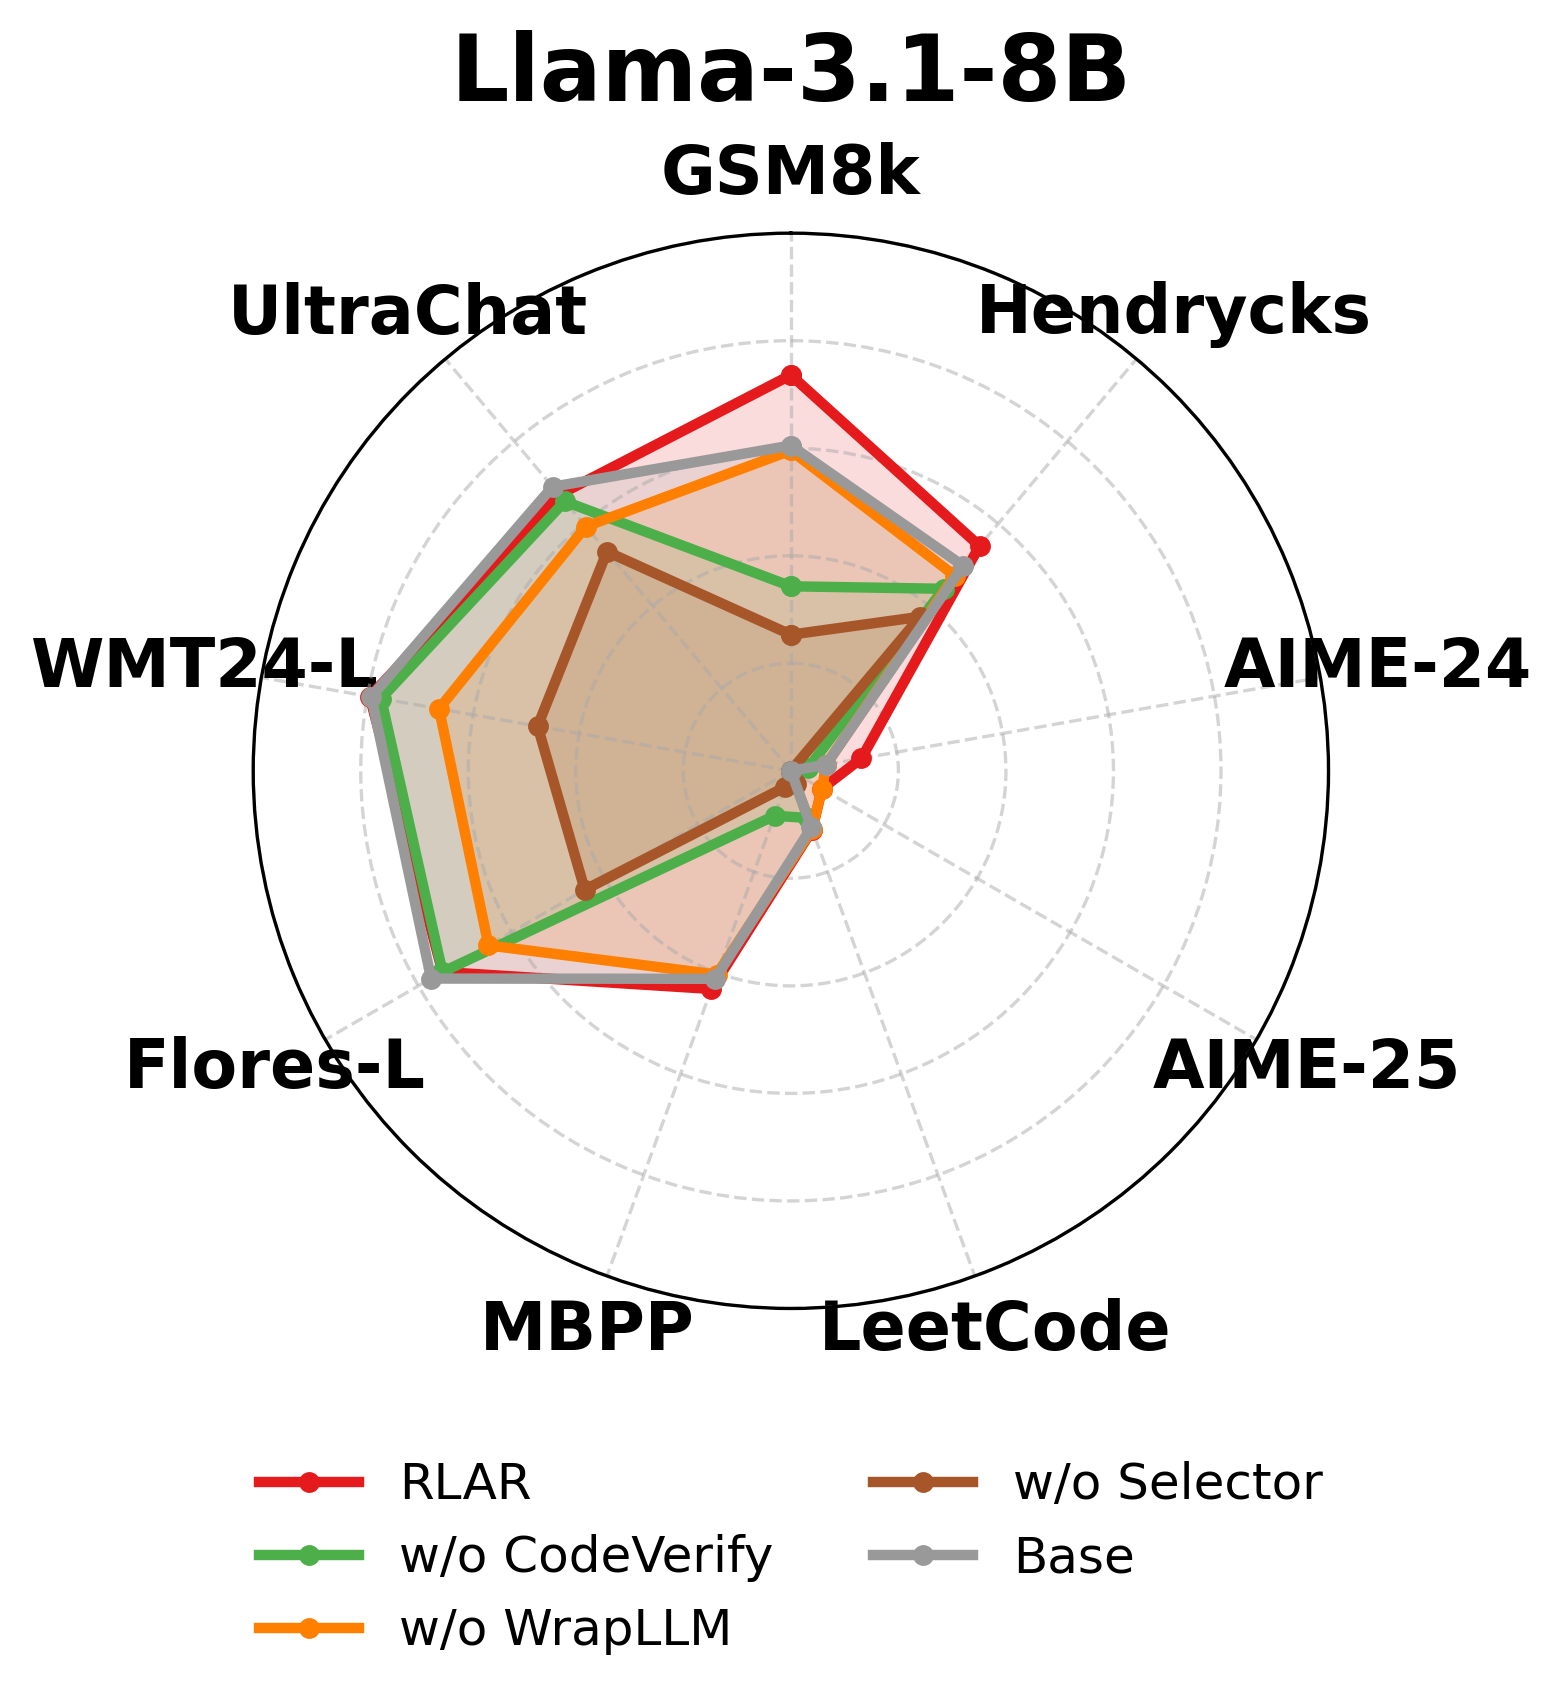
\includegraphics[width=\linewidth]{Figures/llama_ablation.png}
        \caption{Llama-3.1-8B}
        \label{fig:abl_llama}
    \end{subfigure}\hfill
    \begin{subfigure}{0.48\linewidth}
        \centering
        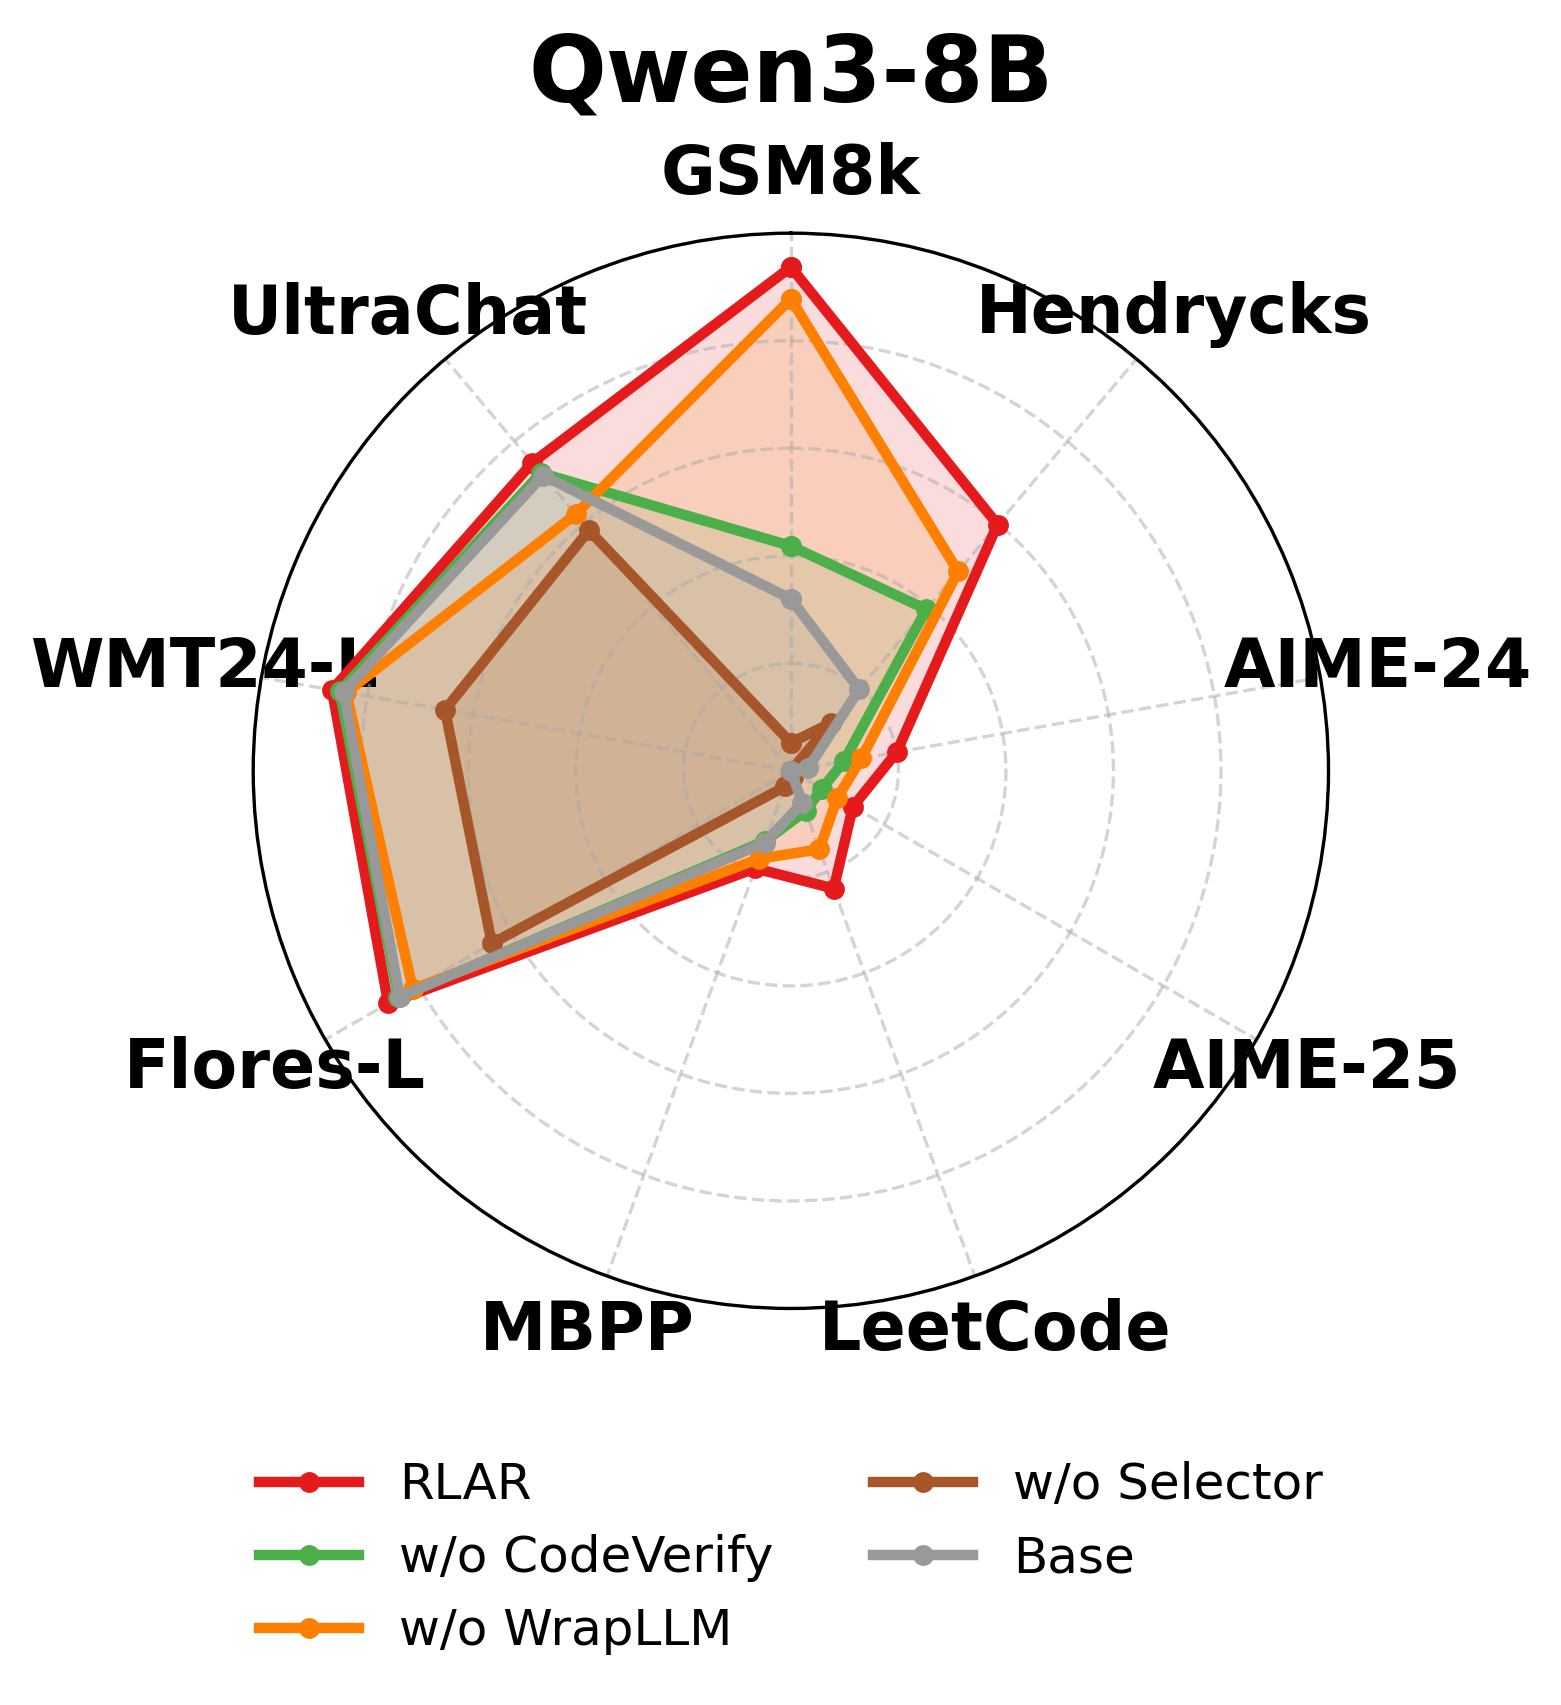
\includegraphics[width=\linewidth]{Figures/qwen_ablation.png}
        \caption{Qwen3-8B}
        \label{fig:abl_qwen}
    \end{subfigure}
    \caption{Ablation studies on Llama-3.1 and Qwen3.}
    \label{fig:ablation}
    \vspace{-4mm}
\end{wrapfigure}




\noindent\textbf{Hack with Verbosity.} \quad
Furthermore, we observe a persistent verbosity bias in LLM-based reward baselines. For example, models trained with GPT-5-Judge consistently produce outputs \(30\%\) \textbf{longer} than those partly learned from rule-based rewards (Human/RLAR). This confirms that verbosity bias is inherently latent in reward LLMs and can be triggered during RL.
Due to its rewarding versatility and the abundant included verifiable rewards, \method{} does not introduce a significant long-tail generation problem.








\subsection{Ablations on Modules}

% \begin{figure}[ht]
%      \centering
%      \begin{subfigure}{0.4\textwidth}
%          \centering
%          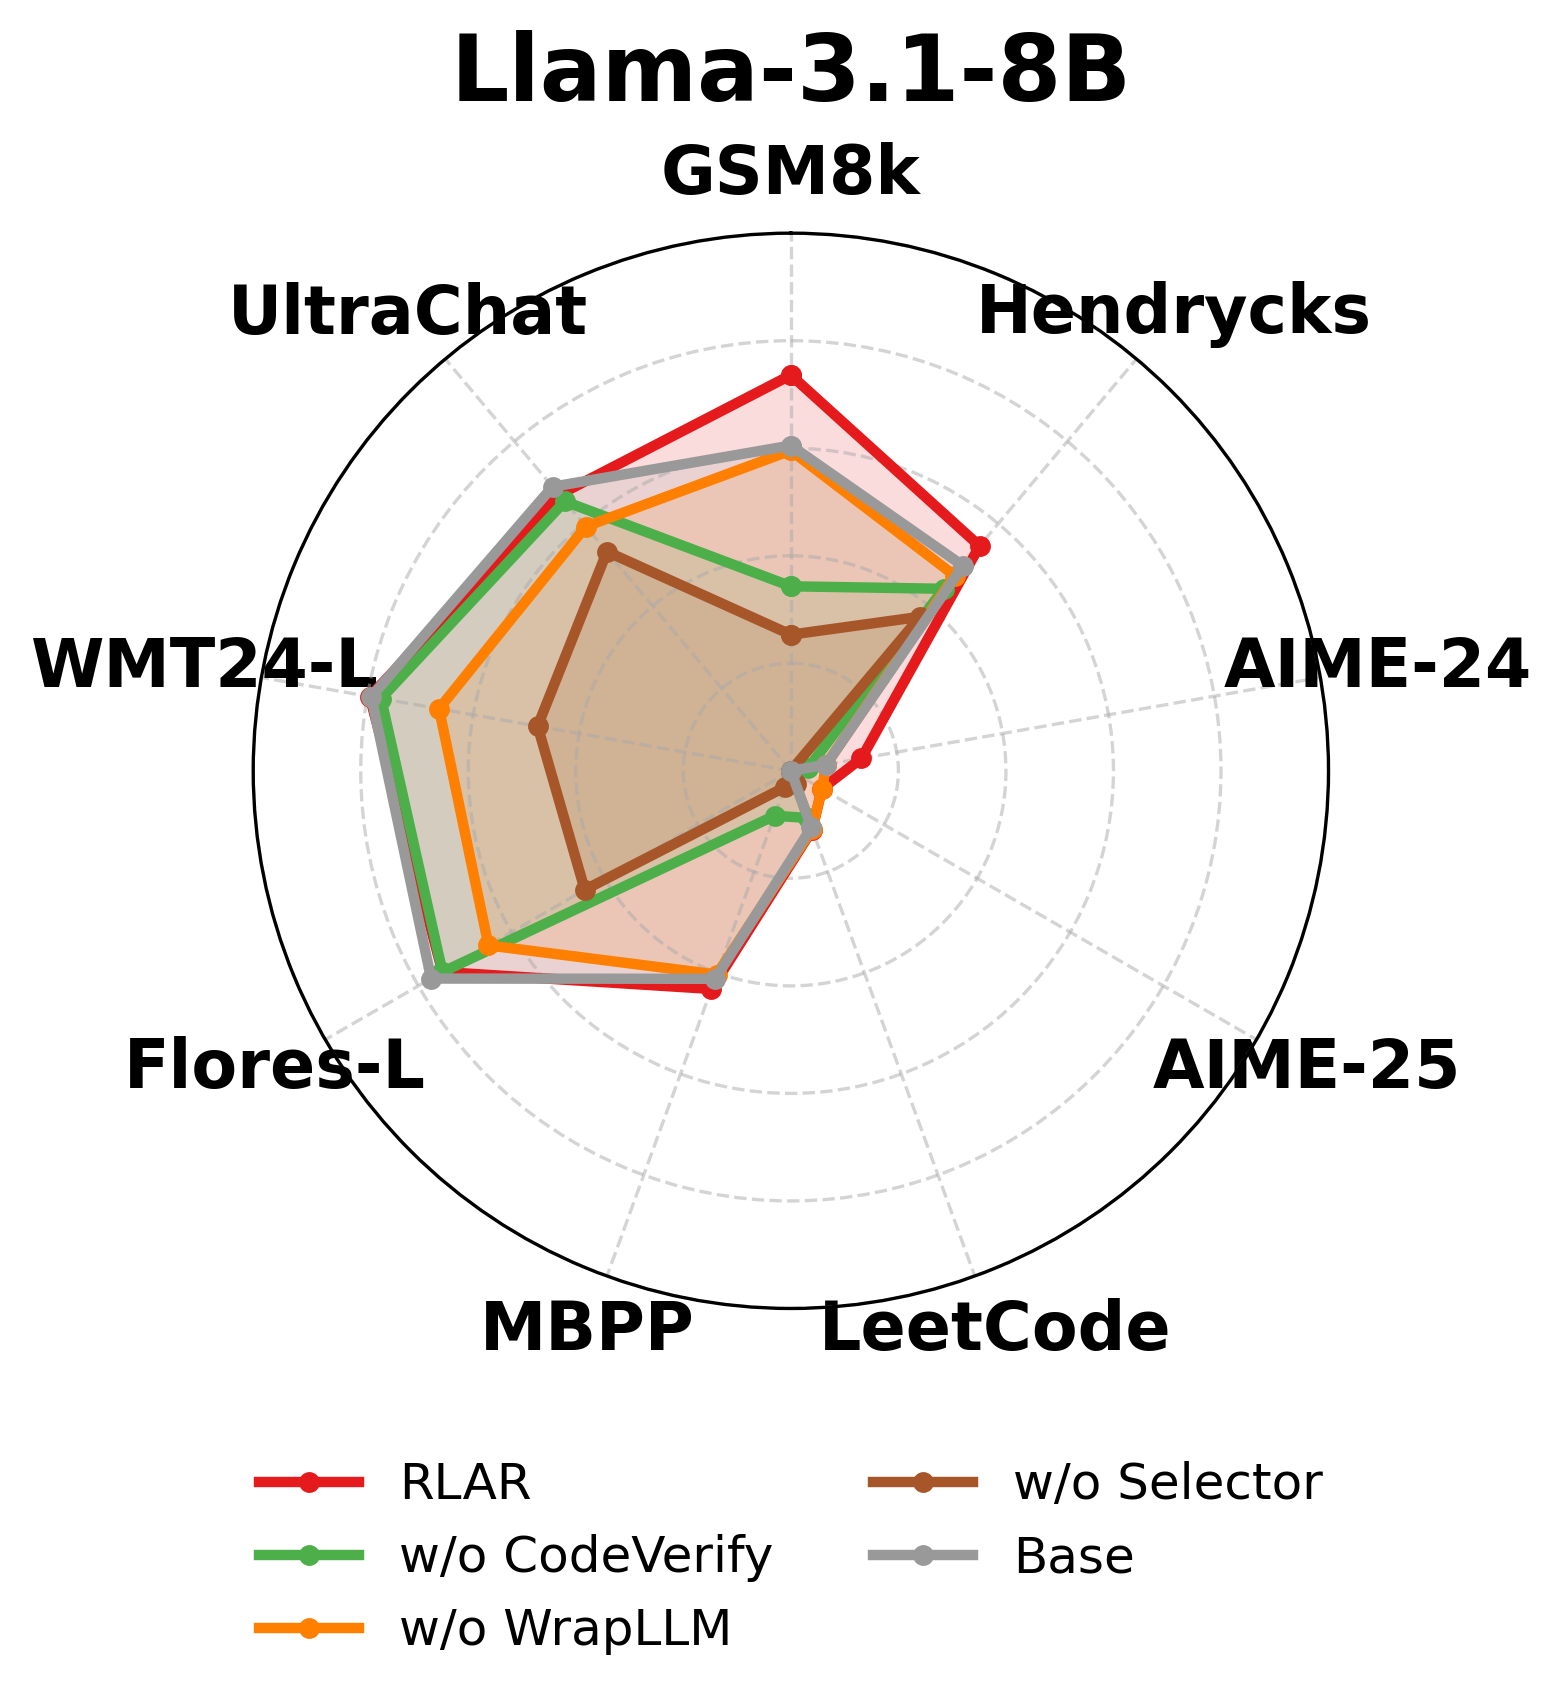
\includegraphics[width=0.8\linewidth]{Figures/llama_ablation.png}
%          \caption{Llama-3.1-8B}
%          \label{fig:abl_llama}
%      \end{subfigure}
%      \hfill
%      \begin{subfigure}{0.4\textwidth}
%          \centering
%          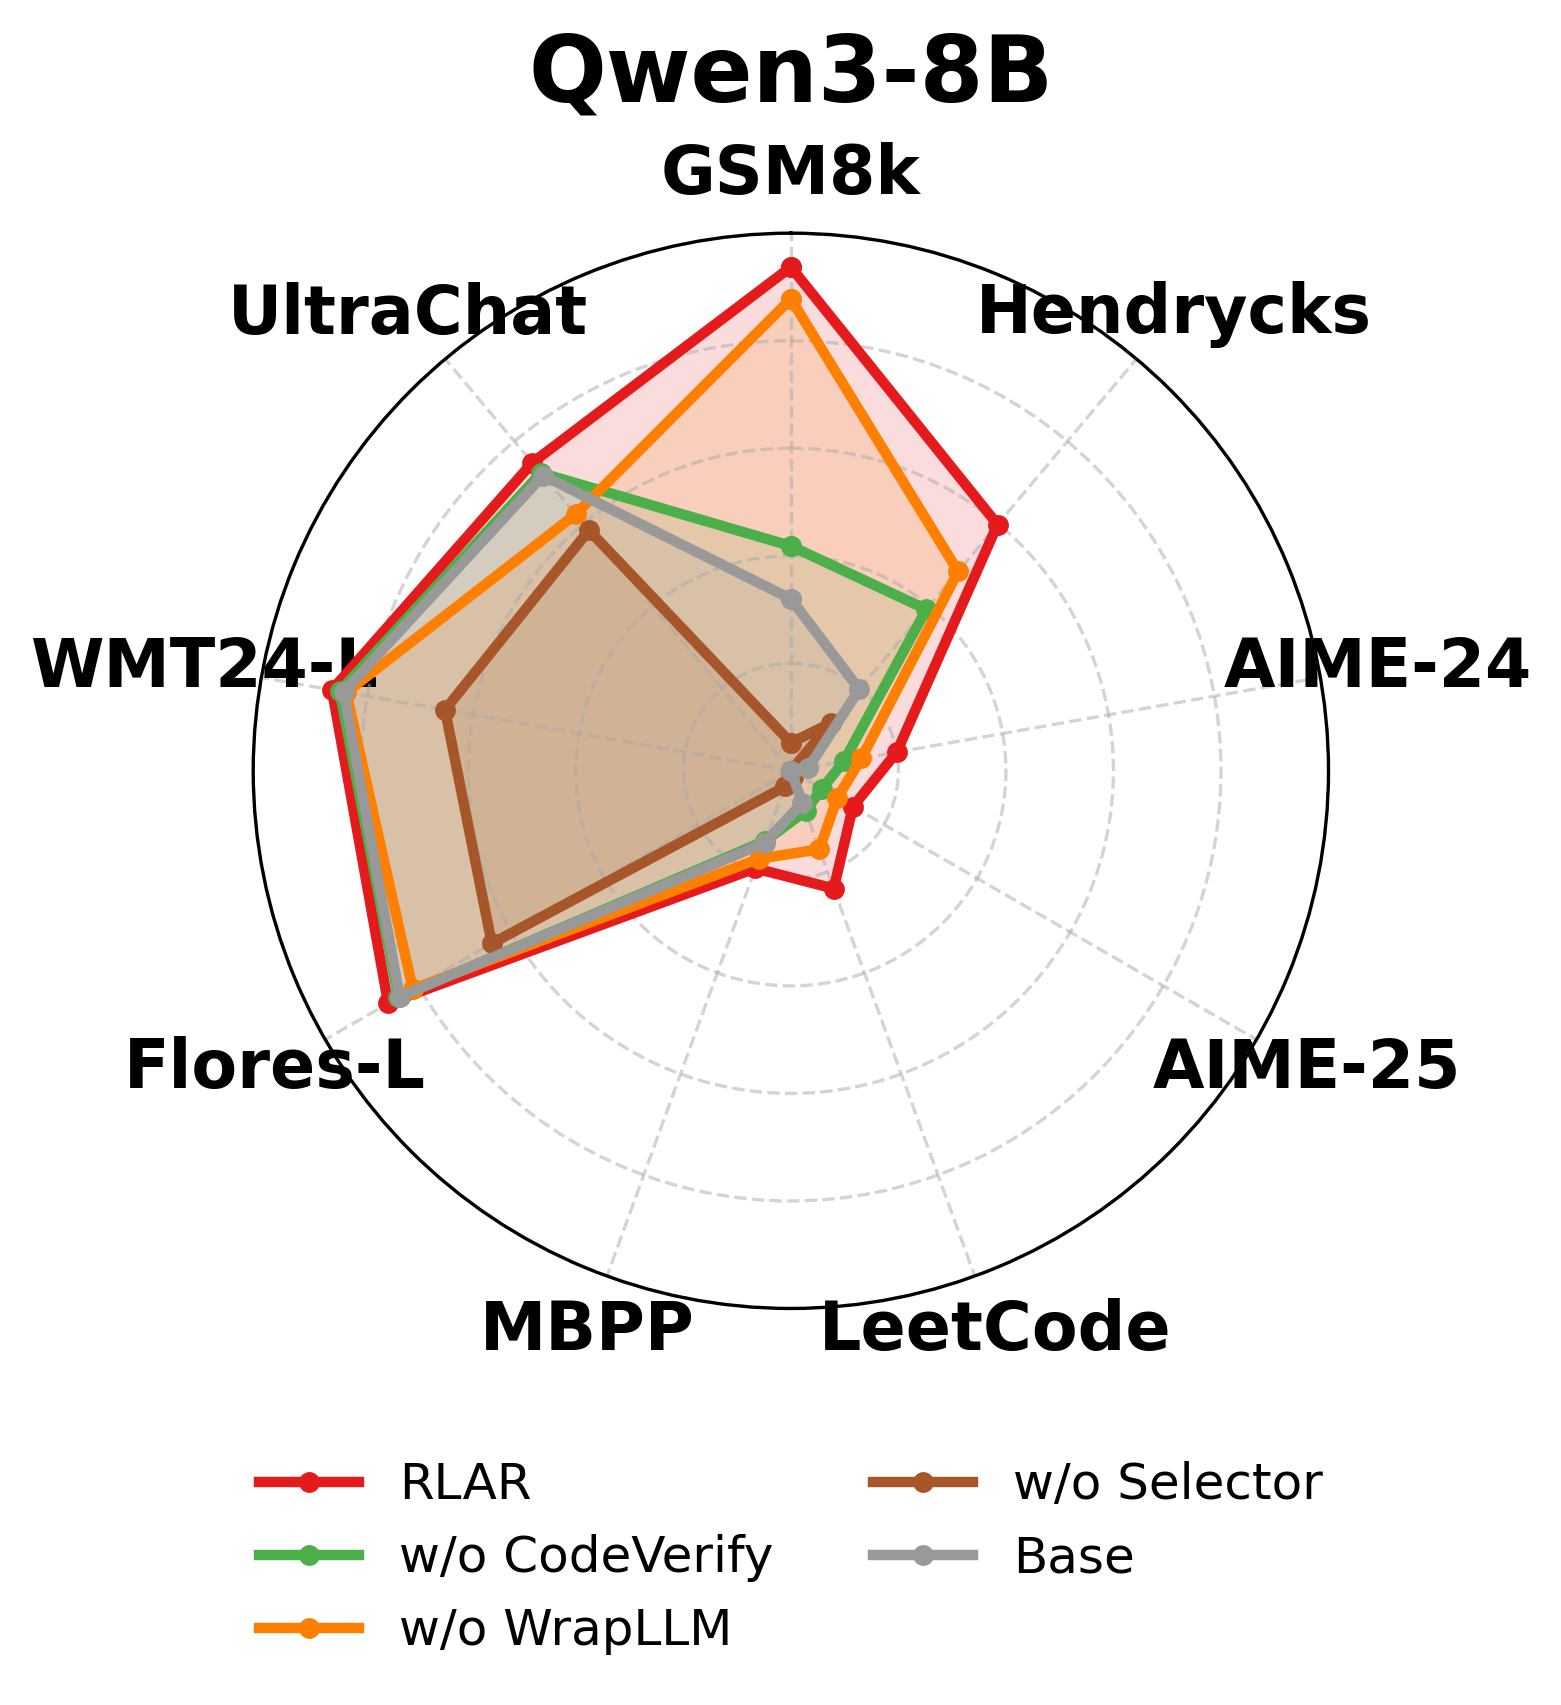
\includegraphics[width=0.8\linewidth]{Figures/qwen_ablation.png}
%          \caption{Qwen3-8B}
%          \label{fig:abl_qwen}
%      \end{subfigure}
%      \caption{Ablation studies on Llama-3.1 and Qwen3.}
%      \label{fig:ablation}
% \end{figure}

To investigate the contribution of each component within the \method{} framework, we conduct an ablation study with the following configurations: (1) \textbf{w/o CodeVerify} and (2) \textbf{w/o WrapLLM}, which respectively disable the corresponding actions in the tool synthesis module; and (3) \textbf{w/o Selector}, where instead of immediate selection post-synthesis, a reward tool is randomly sampled only after all reward tools have been generated. Results of these variants are shown in Figure~\ref{fig:ablation}.

Removing either component of the tool synthesis module consistently results in degradation. Specifically, \textbf{without CodeVerify}-designed tools, mathematical reasoning and coding tasks (\textsc{GSM8k, LeetCode}) drop significantly. \textbf{WrapLLM} is essential for chat and translation tasks. The above results confirm the necessity of query-specific reward designs, which is the core motivation of \method{}. 


Moreover, the Random Reward Selection variant (\textbf{w/o Selector}) underscores the importance of reward matching. The policy degrades on almost all benchmarks. This confirms that appropriate reward selection is crucial in the overall RL training procedure, and that our framework effectively synthesizes high-quality reward tools superior to random alternatives.



% We have further conducted the analysis on the WrapLLM search engine design. The average retrieved model repository position is 5.64 in the first page, showing the relatedness. \textbf{Further error analyses are included in Appendix}~\ref{sec:error_robustness}.

We further analyzed the WrapLLM search engine design. The average retrieved model position is 5.64 on the first page, indicating high relevance. \textbf{Error analyses are in Appendix}~\ref{sec:error_robustness}.


\section{Related Work}


\subsection{LLM RL Reward Designs}


In industry, training \textbf{discriminative} reward models~\citep{ouyangrlhf, deepseekr1, skyworkreward} is widely regarded as the most reliable approach for constructing a human preference oracle within reinforcement learning (RL) frameworks for LLM optimization. In addition, \textbf{generative} rewards extend the aforementioned task from classification to generation, and have demonstrated feasibility in mathematical domains~\citep{generativerm}, RLHF-based settings~\citep{ke-etal-2024-critiquellm, wang2024pandalm, zhu2025judgelm, autoj}, and can be integrated with advances in LLM reasoning, such as CritiqueGRPO~\citep{critiqueGRPO}.
With the rapid development of math reasoning and code generation, the design of \textbf{verifiable} rewards has attracted increasing attention. Binary rewards that can be verified through explicit rules have been shown to be more efficient in these domains~\citep{grpo, tulu3}. \citet{bleuberi} involve employing standard NLP metrics to guide instruction-following alignment as an extension of the aforementioned approach.

\subsection{RL from AI Feedback}


RLAIF~\citep{lee2024rlaif} explores the development of reward models without extensive manual labeling. Self-rewarding~\citep{selfreward} requires the policy model to evaluate and discriminate its own generations. The LLM-as-a-judge paradigm~\citep{mtbench} employs a strong LLM to evaluate another LLM via an evaluation prompt. RewardAgent~\citep{rewardagent} utilizes an LLM to combine pre-specified reward designs. These approaches inevitably embed strong human priors into reward design, either through the evaluation prompt or foundational reward specifications. In contrast to RewardAgent, \method{} extends both design flexibility and evaluation of the reward design framework within an RL algorithm where reward is explicitly formulated (specifically GRPO rather than DPO).

% web agent

\subsection{Dynamic Reward Assigning}



Recent research in integrating LLMs with RL, particularly for reward shaping, primarily focuses on analyzing prior policy traces to iteratively refine the reward function. \citet{afonso2025selfcorrectingrewardshapinglanguage} and \citet{eager-2022} leverage LLM reasoning to guide reward weight pruning or analyze traces to determine appropriate reward shapes. Other methods, such as \citet{logicRL} and \citet{dynamic-rewarding-2024-emnlp}, explore techniques like curriculum scheduling and adjusting the reward schedule via prompt hints.
\method{} diverges by harnessing the LLM's capability to search the web and generate code, directly \textbf{designing entirely new rewards} rather than being limited to weight adjustments. \method{} is also flexible for \textbf{cross-domain optimization} problems, where reward designs differ substantially across sub-domains, a challenge existing single-task-focused methods do not fully address.
\section{Conclusion}

In this paper, we present \method{}, a novel agentic rewarding framework that designs query-specific reward functions for RL algorithms.
By integrating a self-evolving tool library with dynamic synthesis and selection, \method{} achieves superior performance across diverse domains, including math, code, translation, and general chat.
Beyond empirical gains, \method{} demonstrates strong robustness against format and verbosity reward hacking. 
By significantly reducing the costs compared to RLAIF practices, \method{} establishes the ``LLM as Reward Designer'' paradigm.






\bibliographystyle{unsrtnat}
\bibliography{custom}

%%%%%%%%%%%%%%%%%%%%%%%%%%%%%%%%%%%%%%%%%%%%%%%%%%%%%%%%%%%%

\appendix


\label{sec:appendix}

\section{Limitations}

We primarily validate \method{} on heterogeneous tasks in text forms. Due to budget constraints, we did not extend the scope to multi-modal or audio tasks such as text-to-image generation. We believe this is a promising direction for future work. There is still room for further analysis on the scalability of the \method{} framework.

In practice, some repository READMEs may become outdated when reporting (such as claiming to be state-of-the-art at the time of writing). Though not directly caused by the design, \method{} is potentially vulnerable to README hacking, as our assumption is that most of these repository READMEs are trustworthy. We leave the development of more robust retrieval modules for future work.


Lastly, we focus on language models that are modeled as text classifiers. This is quite similar to practices in the industry, mainly aiming to save the computational cost of reward calculation. For generative reward models, our framework can support development on this basis; however, given the constraints of our experimental setup, we consider this to be outside the scope of the present work. 



\section{Broader Impacts and Ethical Considerations}
\label{sec:impact_ethic}


Our research aims to provide positive societal impacts by improving the reliability of reward system design for the reinforcement learning framework in LLM post-training. However, we acknowledge potential negative societal impacts. Like many tuning methods, our approach could theoretically be repurposed for malicious uses, such as exposing malicious reward model checkpoints to \method{} and thereby planting intended deficiencies in the policy LLM.
Furthermore, if \method{} is deployed without careful calibration, it might inherit or amplify biases present in the training data, leading to unfair outcomes for marginalized tasks. We encourage future research to focus on bias mitigation and robustness evaluation before deploying such methods in production environments.

This research conforms in every respect with the NeurIPS Code of Ethics. We have carefully considered the dual-use nature of our work. Because our released code poses a potential risk of misusing public model checkpoint repositories such as HuggingFace and ModelScope, we have implemented the following safeguards.
\paragraph{Originality and Attribution:} The core originality of this work lies in the design and implementation of the \method{} framework. The training outcomes and performance improvements presented in this paper are the combined result of the \method{} architecture and the foundational capabilities of the pre-trained checkpoints we utilized. We explicitly attribute these capabilities to the original authors of the checkpoints, all of which have been appropriately cited. To further ensure transparency, we have documented our execution logs and provided them in Appendix \ref{apd:generated_tools}.
\paragraph{Safeguards and Infrastructure Protection:} To prevent potential misuse of our codebase and protect public infrastructure, we have included explicit usage guidelines in our repository and licensing terms. Crucially, we have disabled automated checkpoint downloading features by default. This design choice prevents our codebase from being exploited to generate excessive or unnecessary network requests (unintentional DDoS) against external model hosting platforms. Furthermore, the external repositories hosting these checkpoints require authenticated user login to utilize their client APIs. This reliance on authentication provides an additional, robust layer of security to prevent the abuse of public network and storage resources.





\section{Reproducibility Statement}

We have included the heterogeneous data construction process in Section~\ref{sec:task_definition} and more details in the Appendix. We describe the RL training settings and experiment platforms in Appendix~\ref{apd:training_details} and Section~\ref{sec:experimental_setup}. The prompts involving the usage of LLM (primarily GPT-4.1) are provided in Appendix~\ref{apd:prompts}. The above materials should be sufficient to reproduce our work.



\section{Data Process Details} \label{apd:data}

\subsection{Detailed Introduction of Datasets}
\noindent\textbf{Translation (En-Fr, Fr-En)}: This task requires the LLM to translate between English and French (in our case, English to French and French to English). We use the dataset \texttt{aircrypto/English-French-Translations-Train-Large}~\citep{hf_enfr} from HuggingFace, which provides high-quality, paired sentence-level samples.

\noindent\textbf{Instruction Following}: Given specific requirements in the provided instructions, the LLM should respond accordingly. We use \texttt{tulu3-sft-reused-on-policy-8b}, part of the Tulu-3~\citep{tulu3} preference dataset, which contains generation pairs between different LLMs during the training of Llama‑3.1‑Tulu‑3‑8B.

\noindent\textbf{Multi-turn}: LLMs respond to instructions with previous interaction histories. We pick \texttt{allenai-WildChat-1M-multiturn}~\citep{allenwilde}, a collection of 1M ChatGPT interaction logs from the wild. We select the English subset aimed at RLHF queries. 

\noindent\textbf{Summarization}: This task requires the LLM to summarize long documents into short abstracts. We pick \texttt{ccdv/govreport-summarization, ccdv/pubmed-summarization, ccdv/arxiv-summarization}~\citep{cohan-etal-2018-discourse-summarizationdataset}, which include different types of documents from arXiv articles to government reports.

\noindent\textbf{Math}: We pick OpenAI \textsc{gsm8k}~\citep{gsm8k}, a classic dataset of grade‑school math problems designed to evaluate multi‑step reasoning. We choose not to use more complex math-reasoning datasets because our focus in this work is primarily on LLM text-generation tasks. Advanced math reasoning often requires specialized methodologies, such as tree‑search reasoning, which makes it unsuitable for single-pass direct generation.

\noindent\textbf{Conditional Generation}: The LLM should generate coherent text according to given constraints. In our setting, we task the LLM with filling in missing paragraphs in an essay or producing a complete essay based on an abstract outline. We use \texttt{qwedsacf/ivypanda-essays}~\citep{ivypanda}, a HuggingFace dataset repository containing long-form essays covering multiple disciplines sourced from the \textit{IvyPanda platform}\footnote{\texttt{https://ivypanda.com/}}.


\subsection{Data Filtering Prompt} ~\label{apd:prompt_for_data_filter}

\begin{tcolorbox}[promptbox, title={DATA\_FILTER\_PROMPT}]
\textbf{Input}: \texttt{task\_samples}, \texttt{quality\_standards}
\tcblower
You are given a set of task samples, each consisting of:
\begin{enumerate}
    \item \textbf{User Query} – the task or request made to the model.
    \item \textbf{Model Response} – the output given by the model.
\end{enumerate}

The samples may come from various task types, including: Translation, Summarization, Math problem solving, RLHF alignment, Conditional text generation, and Multi-turn dialogue.

\textbf{Your Goal}: Identify and select only the samples that did not meet quality standards based on:

\medskip
\textbf{A. Query Quality Issues}:
\begin{itemize}
    \item Ill-formed or incomplete queries; Ambiguous or misleading instructions.
    \item Irrelevant or off-topic requests; Grammatically broken or nonsensical input.
\end{itemize}

\textbf{B. Response Quality Issues}:
\begin{itemize}
    \item Incorrect or factually wrong answers; Incomplete responses.
    \item Poor language quality or incoherent writing.
    \item Hallucinations or made-up facts; Misinterpretation of the query.
\end{itemize}

\textbf{Instructions}:
\begin{enumerate}
    \item For each sample, examine both the query and response.
    \item Mark the sample as \textbf{"Fail"} if either the query quality or the response quality is below standard.
    \item Briefly explain why the sample fails, citing issues in query, response, or both.
    \item Output only the failing samples, in the format:
    \begin{tcolorbox}[colback=white, colframe=gray!20, size=minimal, left=2mm, top=1mm, bottom=1mm]
        \texttt{[Sample ID]} \\
        \texttt{Query: ...} \\
        \texttt{Response: ...} \\
        \texttt{Fail Reason: ...}
    \end{tcolorbox}
\end{enumerate}

\textit{Be strict in applying the criteria — even if only one side (query or response) is substandard, the sample should be considered as failing.}
\end{tcolorbox}
\section{Experiment Training Details} 


\subsection{Training Configuration} \label{sec:training_config}
For the SFT setting, we tuned the base model on the training dataset for 2 epochs. All RL experiments were conducted using the GRPO~\citep{grpo} algorithm framework for 80 steps in total. Since Qwen3-8B is a reasoning model, we enforced a formatting constraint: the reward was set to zero if the reasoning chain failed to be properly encapsulated within `<think>' and `</think>' tags. We did not apply a length penalty during RL training, as generation length does not consistently correlate with task performance. More training details are provided in Appendix~\ref{apd:training_details}.

All experiments were performed on a cluster of 8\(\times\)NVIDIA H100 GPUs (80GB), using a global batch size of 128 and mixed-precision (FP16) training. An auxiliary cluster of 8\(\times\)NVIDIA A100 GPUs (80GB) was dedicated to the deployment and inference of the reward models.



% \subsection{Manual Designed Reward Function over Length}~\label{sec:manual-rm-fun}

% We designed the following function for calculating reward scores over length. Suppose generation length is \(x\) and reference length is \(r\), we raise:
% \begin{widetext}
%     \begin{equation}\label{eq:length_rm}
%     l(x, y) =
%     \begin{cases}
%     \dfrac{x}{r}, \quad 0 \le x \le 0.75r, \\[0.8em]
%     \dfrac{0.25 \left[ f(x; r, 0.25r) - f(0.75r; r, 0.25r) \right] } { \left[ f(r; r, 0.25r) - f(0.75r; r, 0.25r) \right] }
%      \\
%       \quad \quad + 0.75, \quad  x > 0.75r ,
%     \end{cases}
%     \end{equation}
% \end{widetext}

% \begin{align}
% f(t; \mu, \sigma) &=
% \frac{1}{\sqrt{2\pi} \, \sigma}
% \exp\left(
%  -\frac{(t - \mu)^2}{2\sigma^2}
% \right).
% \end{align}

% This can be regarded as stretching and shifting a Gaussian normal probabilistic distribution function, centered at \(r\) with standard deviation \(0.25r\), along the \(y\)-axis so that it passes through the two points \((0.75r, 0.75)\) and \((r, 1)\). Before \(\frac{3}{4}\) of reference length, there is a linear increment with more words.

\subsection{Prompt for the LLM Judge}  
\label{apd:judge_prompt}
\begin{tcolorbox}[
    title = {LLM-as-a-judge Prompt}, 
    breakable, 
    colframe=blue!50!black, 
    colback=blue!10,
    fonttitle=\bfseries
]
\textbf{Input}: \texttt{prompt}, \texttt{candidate}, \texttt{reference}
\tcblower

You are an expert evaluator of language model outputs. You will receive:

\begin{enumerate}
    \item \textbf{Prompt:} The original instruction/task given to the model.
    \item \textbf{Candidate Response:} The model's output to be evaluated.
    \item \textbf{Reference Response:} A high-quality gold-standard or reference output.
\end{enumerate}

\textbf{Your task}:
\begin{itemize}
    \item Evaluate the quality of the \textit{Candidate Response} compared to the \textit{Reference Response} and in relation to the given \textit{Prompt}.
    \item Consider the task category (\textbf{translation}, \textbf{summarization}, \textbf{generation}, \textbf{infilling/cloze}, \textbf{conditional generation}, \textbf{math}, or \textbf{instruction following}) and adjust criteria accordingly.
    \item Score on a scale from \textbf{0 to 10} according to the rubric below.
    \item Output the score in the format \texttt{[[X]]} (where X is the integer) \textbf{once}, followed by a clear explanation.
\end{itemize}

\tcbline % 使用 tcolorbox 的分割线代替 ---

\subsubsection*{Evaluation Dimensions by Task Category}
\textit{(Use whichever are relevant to the given prompt)}

\begin{itemize}
    \item \textbf{Translation}: Accuracy, fidelity, fluency, grammar, style.
    \item \textbf{Summarization}: Coverage, factual faithfulness, conciseness, coherence.
    \item \textbf{Generation}: Relevance, originality, creativity, coherence, style.
    \item \textbf{Infilling/Cloze}: Correctness of missing content, contextual fit, fluency.
    \item \textbf{Math/Reasoning}: Correctness of logic, clarity, rigor of explanation.
    \item \textbf{Instruction Following}: Alignment with intent, completeness.
\end{itemize}

\tcbline

\subsubsection*{Scoring Rubric (0–10)}
\begin{small}
\begin{description}
    \item[10:] \textbf{Perfect}. Fully correct, faithful, and clear. No errors.
    \item[8--9:] \textbf{Very Good}. Minor style issues or tiny, overlookable omissions.
    \item[6--7:] \textbf{Good/Fair}. Mostly correct but with notable small issues or some loss of clarity.
    \item[4--5:] \textbf{Poor/Borderline}. Mix of correct/incorrect; noticeable gaps; low reliability.
    \item[1--3:] \textbf{Very Poor}. Incoherent, irrelevant, or almost entirely wrong.
    \item[0:] \textbf{No meaningful output} or completely unrelated.
\end{description}
\end{small}

\tcbline

\subsubsection*{Output Format}
Respond with:
\begin{tcolorbox}[colback=white, colframe=gray!30, size=minimal, left=2mm, top=2mm, bottom=2mm]
\texttt{[[X]]} \\
\texttt{Explanation:[Detailed explanation within 50 words, citing criteria.]}
\end{tcolorbox}

\tcbline

\textbf{[Prompt]} \\
\texttt{\{prompt\}}

\medskip
\textbf{[Candidate Response]} \\
\texttt{\{candidate\}}

\medskip
\textbf{[Reference Response]} \\
\texttt{\{reference\}}

\end{tcolorbox}




\subsection{Hyperparameters Details for RL Training} \label{apd:training_details}

We use the volcano engine reinforcement learning for LLMs framework, \textsc{verl}~\citep{verlengine}. We validate the implementation of the framework and run all our RL experiments based on it. Below are the hyperparameters for all our experiments and we use the same set of hyperparameters for all experiments.

\begin{table}[htbp]
\centering
\caption{Hyperparameter settings for GRPO training with Qwen3-8B.}
\label{tab:hyperparams}
\small
\begin{tabularx}{\columnwidth}{Xr}
\toprule
\textbf{Category / Parameter} & \textbf{Value} \\
\midrule
\rowcolor[gray]{0.9} \multicolumn{2}{l}{\textit{Training \& Data}} \\
Total Epochs & 5 \\
Global Train Batch Size & 256 \\
Max Prompt Length & 10,000 \\
Max Response Length & 5,000 \\
Truncation Strategy & 'error' \\
Filter Overlong Prompts & True \\
\midrule
\rowcolor[gray]{0.9} \multicolumn{2}{l}{\textit{Algorithm (GRPO/PPO)}} \\
Advantage Estimator & GRPO \\
Learning Rate & $1 \times 10^{-6}$ \\
PPO Mini-batch Size & 16 \\
KL Coefficient & 0.0001 \\
KL Loss Type & low\_var\_kl \\
Entropy Coefficient & 0 \\
KL in Reward & False \\
\midrule
\rowcolor[gray]{0.9} \multicolumn{2}{l}{\textit{Rollout (vLLM Engine)}} \\
Rollout Samples ($n$) & 8 \\
Max Batched Tokens & 65,536 \\
GPU Memory Utilization & 0.7 \\
Prompt/Response Length & 10k / 5k \\
\midrule
\rowcolor[gray]{0.9} \multicolumn{2}{l}{\textit{Parallelism \& Infrastructure}} \\
Nodes / GPUs per Node & 1 / 8 \\
Tensor Parallel (TP) Size & 2 \\
Pipeline Parallel (PP) Size & 4 \\
Gradient Checkpointing & True \\
Micro Batch Size (Actor) & 1 \\
\bottomrule
\end{tabularx}
\end{table}


\begin{table}[t]
\centering
\caption{Hyperparameter settings for GRPO training with Llama-3.1-8B.}
\label{tab:llama_hyperparams}

\small
\begin{tabularx}{\columnwidth}{Xr}
\toprule
\textbf{Category / Parameter} & \textbf{Value} \\
\midrule
\rowcolor[gray]{0.9} \multicolumn{2}{l}{\textit{Training \& Data}} \\
Total Epochs & 5 \\
Global Train Batch Size & 256 \\
Max Prompt Length & 10,000 \\
Max Response Length & 5,000 \\
Truncation Strategy & 'error' \\
Filter Overlong Prompts & True \\
\midrule
\rowcolor[gray]{0.9} \multicolumn{2}{l}{\textit{Algorithm (GRPO)}} \\
Advantage Estimator & GRPO \\
Learning Rate & $1 \times 10^{-6}$ \\
PPO Mini-batch Size & 16 \\
KL Coefficient & 0.0001 \\
KL Loss Type & low\_var\_kl \\
Entropy Coefficient & 0 \\
KL in Reward & False \\
\midrule
\rowcolor[gray]{0.9} \multicolumn{2}{l}{\textit{Rollout (vLLM Engine)}} \\
Rollout Samples ($n$) & 8 \\
Max Batched Tokens & 65,536 \\
GPU Memory Utilization & 0.7 \\
Prompt/Response Length & 10k / 5k \\
\midrule
\rowcolor[gray]{0.9} \multicolumn{2}{l}{\textit{Parallelism \& Infrastructure}} \\
Nodes / GPUs per Node & 1 / 8 \\
Tensor Parallel (TP) Size & 2 \\
Pipeline Parallel (PP) Size & 4 \\
Gradient Checkpointing & True \\
Micro Batch Size (Actor) & 1 \\
\bottomrule
\end{tabularx}
\end{table}


% \begin{lstlisting}[style=mypython]
% python3 -m verl.trainer.main_ppo --config-path=config \
%     --config-name='ppo_megatron_trainer.yaml'\
%     algorithm.adv_estimator=grpo \
%     data.train_files=$rlvr_train_path \
%     data.val_files=$rlvr_test_path \
%     data.train_batch_size=128 \
%     data.max_prompt_length=15000 \
%     data.max_response_length=6000 \
%     actor_rollout_ref.rollout.prompt_length=15000 \
%     actor_rollout_ref.rollout.response_length=6000 \
%     data.filter_overlong_prompts=True \
%     data.truncation='error' \
%     actor_rollout_ref.model.path=$base_model \
%     actor_rollout_ref.actor.optim.lr=5e-6 \
%     actor_rollout_ref.actor.ppo_mini_batch_size=64 \
%     actor_rollout_ref.actor.ppo_micro_batch_size_per_gpu=2 \
%     actor_rollout_ref.actor.megatron.pipeline_model_parallel_size=4 \
%     actor_rollout_ref.actor.megatron.tensor_model_parallel_size=2 \
%     actor_rollout_ref.actor.use_kl_loss=True \
%     actor_rollout_ref.actor.kl_loss_coef=0.001 \
%     actor_rollout_ref.actor.kl_loss_type=low_var_kl \
%     actor_rollout_ref.actor.entropy_coeff=0 \
%     actor_rollout_ref.model.enable_gradient_checkpointing=True \
%     actor_rollout_ref.rollout.log_prob_micro_batch_size_per_gpu=8 \
%     actor_rollout_ref.rollout.tensor_model_parallel_size=1 \
%     actor_rollout_ref.rollout.max_num_batched_tokens=65536 \
%     actor_rollout_ref.rollout.name=vllm \
%     actor_rollout_ref.rollout.gpu_memory_utilization=0.8 \
%     actor_rollout_ref.rollout.n=5 \
%     actor_rollout_ref.ref.log_prob_micro_batch_size_per_gpu=8 \
%     actor_rollout_ref.ref.megatron.pipeline_model_parallel_size=4 \
%     actor_rollout_ref.ref.megatron.tensor_model_parallel_size=2 \
%     algorithm.use_kl_in_reward=False \
%     trainer.critic_warmup=0 \
%     trainer.logger=['console','wandb'] \
%     trainer.project_name=$proj_name \
%     trainer.experiment_name=$exp_name \
%     trainer.n_gpus_per_node=8 \
%     trainer.nnodes=1 \
%     trainer.save_freq=20 \
%     trainer.test_freq=10 \
%     trainer.total_epochs=2 $@
% \end{lstlisting}


% The following is our supervised finetuning training script:

% \begin{lstlisting}[style=mypython]
% torchrun --standalone --nnodes=1 --nproc_per_node=$nproc_per_node \
%      -m verl.trainer.fsdp_sft_trainer \
%     data.train_files=$train_files \
%     data.val_files=$val_files \
%     data.max_length=30000 \
%     data.truncation=left \
%     data.prompt_key=extra_info \
%     data.response_key=extra_info \
%     optim.lr=1e-5 \
%     data.prompt_dict_keys=['question'] \
%     +data.response_dict_keys=['answer'] \
%     data.micro_batch_size=1 \
%     data.micro_batch_size_per_gpu=1 \
%     data.val_batch_size=1 \
%     model.partial_pretrain=$base_model \
%     trainer.default_local_dir=$save_path \
%     trainer.project_name=main_exp \
%     trainer.experiment_name=sft-qwen3-0.6 \
%     trainer.logger=['console'] \
%     trainer.total_epochs=2 \
%     trainer.default_hdfs_dir=null $@ \
%     ulysses_sequence_parallel_size=2 \
%     use_remove_padding=true
% \end{lstlisting}

The other hyperparameters, such as optimizer $\beta$, are set to the defaults from the framework trainer configurations at \url{https://github.com/volcengine/verl/tree/main/verl/trainer/config}.

\section{Prompt Details} \label{apd:prompts}

\subsection{Prompt for Task Decomposition}  \label{apd:prompt_task_decpm}

\begin{tcolorbox}[title = {Task\_Decomposition\_Prompt}, breakable, colframe=blue!50!black, colback=blue!10]
\textbf{Input}: original\_task
\tcblower

Please break down the following generative task into a combination of several basic generative tasks:  

Basic task list:
1. Controlled generation: Generate coherent natural language text that meets certain given conditions. Best for simple, clear tasks; complex writing should be split into smaller steps like planning and cloze generation.

2. Translation: Generate a corresponding text in another natural language from a text in one natural language.  

3. Text summarization: Summarize the given text, retaining the main information.  

4. Question answering: Provide appropriate answers based on background information and question requests provided by the user.  

5. Paraphrasing: Modify the provided text into a different form of expression that meets the given rewriting requirements.  

6. Cloze generation: Given a continuous piece of text with missing parts, generate appropriate text for the missing positions so that the original text becomes complete, coherent, and consistent.  

7. Planning generation: Plan a high-level outline in order to accomplish a relatively complex generative task, such as creating a chapter list, designing character traits, designing scripts, or designing a timeline.  

8. Code: Generate executable code that meets the specified requirements, or supplement or revise code according to the given requirements. The defining criterion for this task is that the output is primarily code.


Decomposition goal:


- Break down the complex generative task provided by the user into a list composed of the above basic tasks according to its logical steps.  
- Steps should be arranged in execution order, and the description should start from the original input form and proceed until the task is completed.  

- Each step must clearly specify the “basic task type” and the execution content of that step.  

- If the task does not need to be broken down, provide a single-step basic task and rewrite its description into a clearer instruction that aligns with the type of task in the basic task list.


Output format requirements:

- List the decomposition results step-by-step (step number + basic task type name + specific execution description). 

- Enclose the final result within $<$Result$>$ ... $<\backslash$Result $>$  tags.  

Below is an example:  


[Example Start]  


Task to be decomposed: Please provide an English summary for the following Chinese document.

Decomposition result:  

1. Translation: Please translate the following Chinese document into an English document.  

2. Text summarization: Please summarize the given English document, and ensure the summary does not exceed 200 words.  

[Example End]  

Now, perform the above decomposition process on the given question (or task description) below, and write the final decomposition result within $<$Result$>$ ... $<\backslash$Result $>$  tags.

\{original\_task\}

\end{tcolorbox}





\subsection{Prompt Details for Reward Model Choice}

\subsubsection{Search API Tool} \label{apd:tool_snippet}

\begin{lstlisting}[style=mypython]
{
    "type": "function",
    "function": {
        "name": "search_serper_engine",
        "description": "Performs a Google search using the Serper API restricted to finding Hugging Face model checkpoints. Use this tool only to look up Hugging Face checkpoint URLs, model pages, or related information. Short queries work best. Reward model might be confusing with base models or chat models",
        "parameters": {
            "type": "object",
            "properties": {
                "query": {
                    "type": "string",
                    "description": "The search query for Hugging Face checkpoints, e.g., model names or keywords to locate on huggingface.co."
                }
            },
            "required": ["query"]
        }
    }
}
\end{lstlisting}



\subsubsection{Prompt for search results filtration}  
\label{apd:filter_prompt}
\begin{tcolorbox}[title = {Search Results Filtration}, breakable, colframe=blue!50!black, colback=blue!10]
\textbf{Input}: \texttt{original\_task}
\tcblower

You are given a list of search engine results with position IDs. 

Your task is to filter them according to the following rules:

\begin{enumerate}
    \item \textbf{Identify Reward Models:} 
    \begin{itemize}
        \item Keep only results that are \textbf{reward model} links.
        \item Reward models often have model names containing keywords like \texttt{-Reward-} or \texttt{-RM-}.
        \item Discard results for base models (\texttt{-Base}), instruct models (\texttt{-Instruct}), or chat models (\texttt{-Chat}).
        \item If a model name has none of these hints, and it's unclear whether it is a reward model, discard it.
    \end{itemize}

    \item \textbf{Hugging Face Model Repositories Only:}
    \begin{itemize}
        \item Keep only links pointing to \textbf{Hugging Face model repositories}.
        \item Discard datasets, research papers, blog posts, or other non-model content.
    \end{itemize}

    \item \textbf{Score Output Format only:}
    \begin{itemize}
        \item Regression models only, in other words, models that output a score (e.g., 0--1) rather than generating text.
    \end{itemize}
\end{enumerate}

Directly discard those items that violate rule 1, 2, or 3 and keep the rest. Output the remaining items in a list using their original position IDs like \texttt{[0, 1, 3, 5, ...]}. If none of the items are left, output an empty list \texttt{[]}.

\bigskip
\{results\}

\end{tcolorbox}




\subsubsection{Prompt for search results Reranking}  
\label{apd:rerank_prompt}


\begin{tcolorbox}[title = {Search Results Reranking}, breakable, colframe=blue!50!black, colback=blue!10]
\textbf{Input}: \texttt{original\_task}
\tcblower

You are given a list of search engine results with position IDs.  
Your task is to filter and rank them according to the following rules:

\begin{enumerate}
    \item \textbf{Identify Reward Models:}  
    \begin{itemize}
        \item Keep only results that are \textbf{reward model} links.  
        \item Reward models often have model names containing keywords like \texttt{-Reward-} or \texttt{-RM-}.  
        \item Discard results for base models (\texttt{-Base}), instruct models (\texttt{-Instruct}), or chat models (\texttt{-Chat}).  
        \item If a model name has none of these hints, and it's unclear whether it is a reward model, discard it.
    \end{itemize}

    \item \textbf{Hugging Face Model Repositories Only:}  
    \begin{itemize}
        \item Keep only links pointing to \textbf{Hugging Face model repositories}.  
        \item Discard datasets, research papers, blog posts, or other non-model content.
    \end{itemize}

    \item \textbf{Score Output Format only:}
    \begin{itemize}
        \item Regression models only; in other words, models that output a score (e.g., 0--1) rather than generating text.
    \end{itemize}
\end{enumerate}

Directly discard those items that violate rule 1, 2, or 3 and keep the rest. Output the remaining items in a list using their original position IDs, sorted by relevance, like \texttt{[0, 1, 3, 5, ...]}. If none of the items are left, output an empty list \texttt{[]}.

\bigskip
\{results\}

\end{tcolorbox}




\subsubsection{Prompt for search results LLM-based Reward Model Implementation}  
\label{apd:implement_prompt}


\begin{tcolorbox}[title = {Reward Tool Implementation}, breakable, colframe=blue!50!black, colback=blue!10]
\textbf{Input}: original\_task
\tcblower


Implement a python script for launching a reward model according to the following informative scripts. The model local checkpoint is \{model\_local\_dir\}. The cuda device for the model is "\{cuda\_device\}". You should write a function, that support input parameter:
- prompt: str, instruction or context conditions
- response: str, the text need to be evaluated
- reference: str, some reference answer/response for the above prompt

Your implementation are free to use the packages mentioned in the scripts. Name the calculation function starting with "compute\_", such as "def compute\_XXX(...)" where XXX should be the reward model name or related abbreviation. Make sure the model checkpoint is loaded precisely once in the script. Format your output enclosed within "python $\backslash$ n xxxx $\backslash$n". Also, additionally print the calculation funciton after four sharp marks \#\#\#\#, such as "\#\#\#\# def compute\_xxx(...)" in the end of your output (outside the python script).

\{scripts\}

[your implementation]

\end{tcolorbox}



\subsection{Prompt for Code-Agent workflow}

\subsubsection{Plan} \label{sec:code-agent-plan}


\begin{tcolorbox}[promptbox, title={LIST\_TASK\_PROMPT}]
\textbf{Input}: \texttt{\{task\}}
\tcblower
You are an expert in designing reward models and evaluation metrics for the \textbf{\{task\}} task.  
Your goal is to list \textbf{3–5 possible reward model or evaluation metric choices} for this task, drawing from the following two categories:  

\begin{enumerate}
    \item \textbf{Rule-based} – Explicit rules (e.g., exact match with reference output, length constraints) used directly as rewards.  
    \item \textbf{Metric-based} – Standard NLP metrics (e.g., BLEU, ROUGE, METEOR) used to evaluate and reward generated results.  
\end{enumerate}

\textbf{Output formatting requirements}:  
\begin{itemize}
    \item Place your results \textbf{after four hash marks (\texttt{\#\#\#\#})}.
    \item For \textbf{each choice}, indicate its \textbf{category} and \textbf{name}, using the format:
    \begin{quote}
        \texttt{\#\#\#\# <Category>/<Name>: <Brief description>}
    \end{quote}
    \item Use a \textbf{new line} for each choice.
\end{itemize}

\textbf{Example}:  
\begin{tcolorbox}[colback=white, colframe=gray!30, size=small]
\texttt{\#\#\#\# Metric-based/BLEU: Measures the n-gram overlap between generated output and reference text.}\\
\texttt{\#\#\#\# Rule-based/Length: Rewards outputs within the target length range for conciseness.}
\end{tcolorbox}
\end{tcolorbox}




\subsubsection{Write} \label{sec:code-agent-write}

\begin{tcolorbox}[title={\texttt{WRITE\_CODE\_PROPMT}}, breakable, colframe=blue!50!black, colback=blue!5]
Implement the following metric according to description using python. Write a function begin with \texttt{'compute\_xxx'}. The function accepts: \texttt{prompt}, \texttt{candidate\_response}, \texttt{reference\_response}. Return a scalar score.

Output the python code in \texttt{```python ... ```}. List requirements in \texttt{requirements.txt} style.

\medskip
\texttt{[metric description]}
\end{tcolorbox}




\subsection{Prompts for WrapLLM and CodeVerify} \label{apd:prompt_wrap_code}


% --- TASK_CLS_PROMPT ---
\begin{tcolorbox}[title={\texttt{TASK\_CLS\_PROMPT}}, breakable, colframe=blue!50!black, colback=blue!5]
You will be given a \texttt{question} and an \texttt{answer} from a language model interaction.  
Your job is to determine the main type of task being performed. Examples include but are not limited to: translation, summarization, question answering, code generation, math solving, creative writing, RLHF alignment, explanation, classification, etc.  
You do not need to list all possible task types — instead, use your judgment to give the most fitting label for this specific instance.  
\textbf{Rules:}  
\begin{enumerate}
    \item Output only the task type as a concise label (maximum \textbf{three words}).
    \item Do not include any extra text, punctuation, or explanation.
    \item If uncertain, choose the closest-fitting description.
\end{enumerate}

Provide your output results after four sharp marks \texttt{\#\#\#\#}, such as \texttt{"\#\#\#\# Translation"}.

\textbf{Input example:}  
\begin{quote}
\texttt{"question": "You are a helpful assistant that translates English sentences to French... [English Input]\textbackslash n Michael Gill formed The Murder Mile... [French Output]\textbackslash n",} \\
\texttt{"answer": "Michael Gill a formé The Murder Mile..." }
\end{quote}
\textbf{Output:}  
\texttt{\#\#\#\# English--French Translation}

Now classify the given instance according to these rules.
\end{tcolorbox}

% --- TASK_DECOMP_PROMPT ---
\begin{tcolorbox}[title={\texttt{TASK\_DECOMP\_PROMPT}}, breakable, colframe=blue!50!black, colback=blue!5]
Please break down the following generative task into a combination of several basic generative tasks:

\textbf{Basic task list:}
\begin{enumerate}
    \item \textbf{Controlled generation:} Generate coherent natural language text that meets certain conditions.
    \item \textbf{Translation:} Generate corresponding text in another natural language.
    \item \textbf{Text summarization:} Summarize the given text.
    \item \textbf{Question answering:} Provide appropriate answers based on background info.
    \item \textbf{Paraphrasing:} Modify text into a different form of expression.
    \item \textbf{Cloze generation:} Fill in missing parts of a text.
    \item \textbf{Planning generation:} Plan a high-level outline (chapter lists, scripts).
    \item \textbf{Code:} Generate or revise executable code.
\end{enumerate}

\textbf{Decomposition goal:}
\begin{itemize}
    \item Break down the complex task into a list of the above basic tasks.
    \item Steps should be in execution order.
    \item Each step must specify the ``basic task type'' and execution content.
\end{itemize}

\textbf{Output format requirements:}
\begin{itemize}
    \item List results step-by-step (step number + type + description).
    \item Enclose the final result within \texttt{<Result> ... </Result>} tags.
\end{itemize}

\bigskip
\texttt{\{original\_task\}}
\end{tcolorbox}

% --- LIST_TASK_PROMPT ---
\begin{tcolorbox}[title={\texttt{LIST\_TASK\_PROMPT}}, breakable, colframe=blue!50!black, colback=blue!5]
You are an expert in designing reward models and evaluation metrics for the \textbf{\texttt{\{task\}}} task.  
Your goal is to list \textbf{3--5 possible reward model or evaluation metric choices}, drawing from:  
\begin{enumerate}
    \item \textbf{Rule-based} -- Explicit rules (e.g., exact match, length constraints).
    \item \textbf{Metric-based} -- Standard NLP metrics (e.g., BLEU, ROUGE).
\end{enumerate}

\textbf{Output formatting requirements:}  
\begin{itemize}
    \item Place your results \textbf{after four hash marks (\texttt{\#\#\#\#})}.
    \item Format: \texttt{\#\#\#\# <Category>/<Name>: <Brief description>}
    \item Use a \textbf{new line} for each choice.
\end{itemize}
\end{tcolorbox}

% --- WRITE_CODE_PROPMT ---
\begin{tcolorbox}[title={\texttt{WRITE\_CODE\_PROPMT}}, breakable, colframe=blue!50!black, colback=blue!5]
Implement the following metric according to description using python. Write a function begin with \texttt{'compute\_xxx'}. The function accepts: \texttt{prompt}, \texttt{candidate\_response}, \texttt{reference\_response}. Return a scalar score.

Output the python code in \texttt{```python ... ```}. List requirements in \texttt{requirements.txt} style.

\medskip
\texttt{[metric description]}
\end{tcolorbox}

% --- WRAP_TOOL_PROMPT ---
\begin{tcolorbox}[title={\texttt{WRAP\_TOOL\_PROMPT}}, breakable, colframe=blue!50!black, colback=blue!5]
Write a short description of the following reward function. Briefly explain what it calculates and how to use it for NLP evaluation.

\textbf{NAME:} \texttt{\{name\}} \\
\textbf{CODE:} \\
\texttt{```python} \\
\texttt{\{code\}} \\
\texttt{```}

Write your description after \texttt{\#\#\#\#}, e.g., \texttt{"\#\#\#\# This function calculates..."}.
\end{tcolorbox}

% --- METRIC_DESIGN_PROMPT ---
\begin{tcolorbox}[title={\texttt{METRIC\_DESIGN\_PROMPT}}, breakable, colframe=blue!50!black, colback=blue!5]
You are an expert in designing evaluation metrics with python. Implement \texttt{\{metric\}}. 

\textbf{Info:} \texttt{\{info\}}

Write a function \texttt{def compute\_XXX(prompt, candidate\_response, reference\_response)} that returns the score. Enclose in \texttt{```python ... ```}.
\end{tcolorbox}

% --- REWARD_MODEL_DESIGN_PROMPT ---
\begin{tcolorbox}[title={\texttt{REWARD\_MODEL\_DESIGN\_PROMPT}}, breakable, colframe=blue!50!black, colback=blue!5]
Expert in reward models. Write a script to calculate reward scores. 
Function: \texttt{def compute\_XXX(prompt, response, reference)}. 
Device: \texttt{"cuda:0"}. Load model precisely once.

\textbf{README.md:} \texttt{\{readme\}} \\
\textbf{Path:} \texttt{\{model\_path\}}
\end{tcolorbox}

% --- RERANK_PROMPT ---
\begin{tcolorbox}[title={\texttt{RERANK\_PROMPT}}, breakable, colframe=blue!50!black, colback=blue!5]
Filter search results based on:
\begin{enumerate}
    \item \textbf{Identify Reward Models:} Keep \texttt{-Reward-} or \texttt{-RM-}. Discard \texttt{-Base}, \texttt{-Instruct}, \texttt{-Chat}.
    \item \textbf{Hugging Face Only:} Model repositories only. Discard datasets/papers.
    \item \textbf{Score Output:} Regression models (e.g., 0--1).
\end{enumerate}
Output original IDs as a list: \texttt{[0, 1, 3]}.

\medskip
\texttt{\{results\}}
\end{tcolorbox}

% --- LLMRM_IMPLEMENT_CODE ---
\begin{tcolorbox}[title={\texttt{LLMRM\_IMPLEMENT\_CODE}}, breakable, colframe=blue!50!black, colback=blue!5]
Implement python script for reward model. \\
\textbf{Checkpoint:} \texttt{\{model\_local\_dir\}} \\
\textbf{Device:} \texttt{"\{cuda\_device\}"} \\
\textbf{Function:} \texttt{def compute\_XXX(prompt, response, reference)}.

Format: \texttt{```python ... ```}. Print function signature after \texttt{\#\#\#\#} at the end.

\medskip
\texttt{\{scripts\}}
\end{tcolorbox}

% --- SELECT_INFORMATIVE_FILES ---
\begin{tcolorbox}[title={\texttt{SELECT\_INFORMATIVE\_FILES}}, breakable, colframe=blue!50!black, colback=blue!5]
Identify informative files from HF repo: \\
\texttt{\{file\_list\}}

Output list: \texttt{["file1.py", "README.md"]}. No extra text.
\end{tcolorbox}
\section{LLM usage in this paper} \label{apd:llm_usage}


Large Language Models (LLMs) were used in the preparation of this work as a general-purpose assistance tool. Specifically, LLMs were employed in the following ways:
\begin{itemize}
    \item \textbf{Translation Assistance}: Converting expressions and sentences from the author’s native language into English.
    \item \textbf{Language Polishing and Grammar Revision}: Improving clarity, fluency, and grammatical correctness of the text, and ensuring that phrasing is natural in academic English.
    \item \textbf{Draft Review and Critique}: Providing feedback on drafts, including identifying unclear passages, suggesting improvements in structure, and flagging potential ambiguities.
\end{itemize}

LLMs were not used for generating original research ideas, performing data analysis, or writing substantive technical content. All core research contributions, results, and argumentative structure were developed by the authors. The role of LLMs was limited to translation, linguistic polishing, and non-substantive editorial suggestions to improve presentation. 


\section{Historical Generated Tools} \label{apd:generated_tools}

This inventory belongs to the earlier implementation. It is not the fixed API catalogue or the library produced by the revised methodology; those resources require their own versioned experiment manifest.



% \usepackage[margin=1in]{geometry}

% \begin{document}

% \renewcommand{\arraystretch}{1.2} % optional: more row height


{\footnotesize\setlength{\tabcolsep}{3pt}%
\begin{longtable}{|l|l|l|l|}
\caption{A list of the generated reward function tool names by our code-agent.} \label{tab:tool_name_list} \\ \hline 
\textbf{Type} & \textbf{Metric} & \textbf{Type} & \textbf{Metric} \\
\hline
\endfirsthead

\hline
\textbf{Type} & \textbf{Metric} & \textbf{Type} & \textbf{Metric} \\
\hline
\endhead

% --- Table rows ---
rule\_based & \texttt{Forbidden\_Words} & rule\_based & \texttt{Stepwise\_Completeness} \\
rule\_based & \texttt{Prompt\_Adherence} & rule\_based & \texttt{Length} \\
rule\_based & \texttt{Numeric\_Accuracy} & rule\_based & \texttt{Exact\_Template\_Match} \\
rule\_based & \texttt{Novelty\_Penalty} & rule\_based & \texttt{Contradiction\_Detection} \\
rule\_based & \texttt{Disallowed\_Phrase\_Penalty} & rule\_based & \texttt{Exact\_Output\_Match} \\
rule\_based & \texttt{No\_Unsupported\_Claims} & rule\_based & \texttt{Reference\_Match} \\
rule\_based & \texttt{Exact\_Answer\_Match} & rule\_based & \texttt{Named\_Entity\_Preservation} \\
rule\_based & \texttt{Unit\_Consistency} & rule\_based & \texttt{Keyword\_Presence} \\
rule\_based & \texttt{Minimal\_Edit\_Distance} & rule\_based & \texttt{Thesis\_Inclusion} \\
rule\_based & \texttt{Mandatory\_Content\_Inclusion} & rule\_based & \texttt{Scientific\_Claims\_Match} \\
rule\_based & \texttt{Pronounceability} & rule\_based & \texttt{Position\_Sensitivity} \\
rule\_based & \texttt{Section\_Coverage} & rule\_based & \texttt{Entity\_Presence} \\
rule\_based & \texttt{Answer\_Type\_Match} & rule\_based & \texttt{Stepwise\_Correctness} \\
rule\_based & \texttt{Terminology\_Accuracy} & rule\_based & \texttt{Diversity\_Score} \\
rule\_based & \texttt{Forbidden\_Content} & rule\_based & \texttt{Fact\_Match} \\
rule\_based & \texttt{Forbidden\_Phrase\_Detection} & rule\_based & \texttt{No\_Information\_Leakage} \\
rule\_based & \texttt{Annotation\_Completeness} & rule\_based & \texttt{Grammar\_and\_Spelling\_Accuracy} \\
rule\_based & \texttt{Clarity\_Constraint} & rule\_based & \texttt{Answer\_Presence} \\
rule\_based & \texttt{No\_Overlap\_with\_Input} & rule\_based & \texttt{No\_Syntax\_Errors} \\
rule\_based & \texttt{Numeric\_Tolerance} & rule\_based & \texttt{Edit\_Distance} \\
rule\_based & \texttt{Keyword\_Coverage} & rule\_based & \texttt{No\_Repetition} \\
rule\_based & \texttt{Length\_Ratio} & rule\_based & \texttt{One-Hot\_Accuracy} \\
rule\_based & \texttt{Novelty} & rule\_based & \texttt{Exact\_Match} \\
rule\_based & \texttt{Pattern\_Compliance} & rule\_based & \texttt{Step\_Match} \\
rule\_based & \texttt{Syntax\_Validity} & rule\_based & \texttt{Format\_Compliance} \\
rule\_based & \texttt{Allowed\_Vocabulary} & rule\_based & \texttt{Entity\_Overlap} \\
rule\_based & \texttt{Explicit\_Irrelevance} & rule\_based & \texttt{Accuracy} \\
rule\_based & \texttt{Coverage\_of\_Key\_Points} & rule\_based & \texttt{Section\_Presence} \\
rule\_based & \texttt{Clarity} & rule\_based & \texttt{Test\_Case\_Pass\_Rate} \\
rule\_based & \texttt{Dictionary\_Filtering} & rule\_based & \texttt{Length\_Expansion} \\
rule\_based & \texttt{Content\_Inclusion} & rule\_based & \texttt{Error\_Pattern\_Removal} \\
rule\_based & \texttt{Plagiarism\_Check} & rule\_based & \texttt{Functionality\_Test} \\
rule\_based & \texttt{Politeness\_Constraint} & rule\_based & \texttt{Formatting\_Compliance} \\
rule\_based & \texttt{Exact\_Test\_Case\_Pass} & rule\_based & \texttt{Key\_Information\_Coverage} \\
rule\_based & \texttt{Genre-Adherence} & rule\_based & \texttt{Passes\_Unit\_Tests} \\
rule\_based & \texttt{Exact\_Step\_Match} & rule\_based & \texttt{Exact\_Keyword\_Match} \\
rule\_based & \texttt{Required\_Field\_Inclusion} & rule\_based & \texttt{Attribute\_Coverage} \\
rule\_based & \texttt{Valid\_Vocabulary} & rule\_based & \texttt{Medical\_Term\_Coverage} \\
rule\_based & \texttt{Keyword\_Absence} & rule\_based & \texttt{Required\_Component\_Presence} \\
rule\_based & \texttt{Final\_Answer\_Correctness} & rule\_based & \texttt{Keyword\_Inclusion} \\
rule\_based & \texttt{Structure\_Compliance} & rule\_based & \texttt{Step\_Consistency} \\
rule\_based & \texttt{Readability} & rule\_based & \texttt{No-Answer\_Accuracy} \\
rule\_based & \texttt{Length\_Constraint} & rule\_based & \texttt{Error\_Reduction} \\
rule\_based & \texttt{Answer\_Type\_Mismatch} & rule\_based & \texttt{Thesis\_Presence} \\
rule\_based & \texttt{Case-Insensitive\_Match} & rule\_based & \texttt{Topic\_Divergence} \\
rule\_based & \texttt{Exact\_Numeric\_Match} & rule\_based & \texttt{Originality-Penalty} \\
rule\_based & \texttt{Keyword\_Exclusion} & rule\_based & \texttt{Structure} \\
rule\_based & \texttt{Format\_Consistency} & rule\_based & \texttt{Required\_Elements} \\
rule\_based & \texttt{Reference\_Citation} & rule\_based & \texttt{Instruction\_Match} \\
rule\_based & \texttt{Key\_Concepts\_Inclusion} & rule\_based & \texttt{Stepwise\_Solution\_Match} \\
rule\_based & \texttt{Fact\_Consistency} & rule\_based & \texttt{Step\_Count\_Constraint} \\
nlp\_metric & \texttt{F1\_Score} & nlp\_metric & \texttt{METEOR} \\
nlp\_metric & \texttt{ROUGE} & nlp\_metric & \texttt{GLEU} \\
nlp\_metric & \texttt{BERTScore} & nlp\_metric & \texttt{M\^{}2\_Score} \\
nlp\_metric & \texttt{chrF} & nlp\_metric & \texttt{ROUGE-L} \\
nlp\_metric & \texttt{Levenshtein\_Distance} & nlp\_metric & \texttt{BLEU} \\
nlp\_metric & \texttt{Distinct-n} & nlp\_metric & \texttt{CodeBLEU} \\
model\_based & \texttt{Content\_Novelty\_Score} & model\_based & \texttt{Negative\_Relevance\_Score} \\
model\_based & \texttt{Topic\_Classifier} & model\_based & \texttt{Perplexity} \\
\hline
\end{longtable}}

\clearpage





\begin{table}[t]
    \centering
    \caption{Successfully Top@9 deployed LLM-based reward models.}
    \label{tab:llm-rm}
    % \resizebox{\linewidth}{!}{
    \begin{tabular}{l|l}
    \hline
\textbf{Source} & \textbf{Repo Name} \\ \midrule
\citep{skyworkreward}   & Skywork/Skywork-Reward-V2-Llama-3.1-8B \\
\citep{skyworkreward}         & Skywork/Skywork-Reward-V2-Qwen3-8B \\
\citep{skyworkreward}         & Skywork/Skywork-Reward-V2-Llama-3.2-3B \\
\citep{skyworkreward}         & Skywork/Skywork-Reward-V2-Qwen3-4B \\
\citep{seedX} & ByteDance-Seed/Seed-X-RM-7B\\
                            & OpenAssistant/reward-model-deberta-v3-base \\
\citep{yang2024gpt2helpful}         & Ray2333/gpt2-large-helpful-reward\_model \\
\citep{nicholas22rewardreward}         & nicholasKluge/RewardModel \\
\citep{cai2024internlm2}         & internlm/internlm2-1\_8b-reward \\
\citep{malik2025rewardbench2advancingreward}         & allenai/Llama-3.1-8B-Base-RM-RB2 \\ \bottomrule
    \end{tabular}
    % }
\end{table}



% \section{Records for Advantage Estimation}

\section{Historical Additional Analysis}

These retained analyses concern the earlier web/code-agent implementation. Repository-retrieval statistics and executability rates do not measure semantic reward quality under the revised protocol in Section~\ref{sec:verification}. They have not been recomputed for the fixed-catalogue design.


%% 附录分析

\subsection{Error and Robustness Analysis} \label{sec:error_robustness}

% 2026-1-1 这边除了 鲁棒性检验，其实应该突出不同顺序 data 进来，框架设计新 reward 的能力 -> 变换数据集呈现顺序，纯随机
% 加一个简单的成本分析

\begin{table}[t]
    \centering
    \caption{Unmatched Task Types by Web Retrieval}
    \label{tab:unmatched_errors}
    \begin{tabular}{lc}
      \toprule
      \textbf{Task Type} & \textbf{Unmatched(\%)}\\
      \midrule
      Infilling & $47.4$ \\
      Essay Generation & $43.8$ \\
      Multi-Turn & $8.8$ \\
      \bottomrule
    \end{tabular}
\end{table}


We conducted an error analysis by counting the task types of instructions for which the Web-Agent could not find a specialized reward model (unmatched conditions). The breakdown in Table \ref{tab:unmatched_errors} shows that the majority of unfound instructions originate from essay infilling/generation tasks. Specifically, there is currently no corresponding reward model explicitly trained for these two task domains, which accounts for the high unmatched ratio in these categories. Notably, when a specialized tool is unmatched, \method{} defaults to using a generic, default LLM-based reward model (\texttt{skywork-llama}).


\begin{table}[t]
    \centering
    \caption{Average Retrieval Position Ranks}
    \label{tab:search_robustness}
    \begin{tabular}{lc}
      \toprule
      \textbf{Category} & \textbf{Avg Pos}\\
      \midrule
      Summ & $7.17$ \\
      Translation & $2.36$ \\
      RLHF & $5.03$\\
      Multi-Turn & $7.61$ \\
      Infill/Gen & $3.75$ \\
      Math & $6.87$ \\
      \bottomrule
    \end{tabular}
\end{table}

To assess the robustness of the searching module, we tracked the average item position (calculated as page rank $\times 10$) for the matched reward model. Across all sampled categories, the overall average retrieval position was $5.64$ items. As detailed in Table \ref{tab:search_robustness}, all individual sub-categories consistently found the optimal item on the first page, confirming the robustness and high precision of the agent's query generation and search logic.

We further validate the soundness of the framework's design by including a detailed analysis of the generated tool quality (Appendix~\ref{sec:gen_tool_quality}) and an investigation into the reward tool usage within our main experiments (Appendix~\ref{sec:reward_tool_usage}). In summary, code-agents achieve a $94.9\%$ executable rate when utilizing rule/metric-based tools, and we observe a dominant percentage of LLM-based reward tool usage in text-generation tasks.



\subsection{Reward Tool Generation Quality} \label{sec:gen_tool_quality}
% \subsection{Tool Generation Stage Unit-Tests}

% We evaluate the quality of reward tools produced by our two agent types (\emph{code agent} and \emph{web agent}) along three axes: (i) \textbf{construct validity} (does the tool implement the intended reward definition for the target task?), (ii) \textbf{operational robustness} (does the tool execute successfully with the fixed interface of \texttt{prompt}/\texttt{candidate}/\texttt{reference} and return a scalar reward without runtime failures?), and (iii) \textbf{reusability} (can the tool be cached and re-applied across queries of the same task type without modification).





We evaluate the quality of reward tools produced by our two agents for tool generation mainly along their construction validity and summarized in Table~\ref{tab:tool_gen_quality}.




\paragraph{Code-agent tools.} 
Across all the training queries, the code agent generated \textbf{118} reward scripts, among which \textbf{112} (\textbf{94.9\%}) were directly executable under our standardized interface.\footnote{Executability is checked by importing the generated function, calling it with a minimal synthetic triplet \texttt{(prompt, candidate, reference)} and verifying a numeric return type without exceptions.}
By type, the set comprises \textbf{102} rule-based functions (\textbf{86.4\%}), \textbf{12} standard metric implementations (\textbf{10.2\%}; e.g., BLEU, METEOR), and \textbf{4} learned-model–based scorers (\textbf{3.4\%}).
Rule-based tools typically encode task-specific verifiable criteria (e.g., numeric-consistency checks for \textsc{GSM8K} or explicit-irrelevance penalties for RLHF-style preference items), while metric-based tools provide length- or n-gram–aware surrogates for general text quality.
We discard learned-model–based proposals from the code agent since they are potential out-of-memory threats to the deploying server.
% as \emph{candidates} but do not enable them by default unless an appropriate lightweight classifier is present locally; this prevents uncontrolled external dependencies from leaking into the code-agent path.

\begin{table}[t]
    \centering
    \caption{Summary of reward tool generation outcomes.}
    \label{tab:tool_gen_quality}
    \begin{tabular}{lc}
    \toprule
    \textbf{Category} & \textbf{Count} \\
    \midrule
    Code-agent scripts (total) & 118 \\
    \quad Executable & 112 (94.9\%)  \\
    \quad Rule-based & 102 (86.4\%) \\
    \quad Metric-based & 12 (10.2\%) \\
    \quad Learned-model–based & 4 (3.4\%) \\
    \midrule
    Web-agent repos (retrieved) & 21 \\
    \quad Deployed & 10 (47.6\%) \\
    \quad Rejected (size) & 2 \\
    \quad Rejected (not classification) & 6 \\
    \quad Rejected (insufficient docs) & 3  \\
    \bottomrule
    \end{tabular}
\end{table}

\paragraph{Web-agent tools.}
The web agent retrieved \textbf{21} candidate repositories from public model hubs (primarily Hugging Face and ModelScope) that matched the predicted task label and satisfied our \emph{reward-model} filter. The filter eliminates base/instruct/chat/vision models and retains text-classification-modeled reward models with download access.
After automatic screening and wrapping, \textbf{10} repositories (\textbf{47.6\%}) were successfully deployed behind a uniform Python API. The remaining \textbf{11} were rejected due to: model size prohibitive for our inference node (\textbf{2}), non–text-classification architectures (\textbf{6}), or insufficient/ambiguous repository documentation for reliable wrapping (\textbf{3}).




% \paragraph{Failure taxonomy and safeguards.}
% For the code agent, non-executable cases were dominated by (a) minor import/path mistakes in metric utilities and (b) boundary cases in string normalization that caused exceptions on empty or malformed inputs.
% We mitigate these by (1) stubbing common NLP utilities with version-pinned fallbacks, (2) adding pre-execution input sanitation, and (3) enforcing a \emph{pure-function} contract (no network I/O, deterministic return).
% For the web agent, deployment rejections primarily reflect \emph{mismatch risk}: models advertised as “reward” are occasionally generic rerankers or multi-modal checkpoints; in addition, sparse READMEs obstruct robust wrapper synthesis.
% Our wrapper generator therefore requires (i) explicit textual classification signatures and (ii) a documented scoring head.

% \paragraph{Reusability and caching.}
% All accepted tools are normalized to a single signature \texttt{score(prompt, candidate, reference) -> float} and registered with a memoized loader.
% During training, the tool registry prevents redundant reconstruction and enables cross-query reuse for the same predicted task type; Section~\ref{sec:final_rm} shows how the policy-facing selector exploits this catalogue to compose proxy rewards on demand.

% \paragraph{Takeaway.}
The high executability of code-agent tools (\textbf{94.9\%}) and the moderate but reliable deployment rate of web-agent tools (\textbf{47.6\%}) indicate that \method{} can \emph{consistently} materialize task-aligned reward functions across heterogeneous inputs.
% This breadth of \emph{operational} reward tools is a prerequisite for the downstream variance reduction and stronger advantages we observe in Section~\ref{sec:analysis_adv} (cf.\ clipping statistics), and underpins the performance gains reported in Table~\ref{tab:main_res}.


% We manually examined the reward calculation scripts generated by our code agents. Among over $8,000+$ training samples, $118$ rule- and metric-based scripts are generated. Among the generated scripts, $112$ of them are executable with the predetermined arguments. We list the whole list of the function names in Table~\ref{tab:tool_name_list}. Among them, $102$ are rule-based calculated, $12$ are standard NLP metrics, such as BLEU~\citep{papineni-etal-2002-bleu}, meteor~\citep{banerjee-lavie-2005-meteor}. This demonstrates the code-agents strong capability when implementing such instruction specific reward functions. $4$ of them, however, appear to be based on learned models, such as classifiers, relevance scores, perplexity.

% Through the web-agents visiting trace, we record that $21$ different repositories are fetched by our search tool. Yet only $10$ of them are successfully deployed as API, due to the following reasons: (1) model size too large to deploy ($2$ repos) (2) filtered out for not being an text-classification model ($6$ repos); (3) lack of informational reademe in target repositories ($3$ repos). We only disclose the successfully deployed repositories in Table~\ref{tab:llm-rm}.

\subsection{Reward Tool Usage and Selection Patterns} \label{sec:reward_tool_usage}
% \subsection{RLVR reward tool selection}
Having established that \method{} can reliably generate and deploy reward tools, we next examine \emph{how} these tools are actually invoked during training.
This analysis addresses two questions: (i) which categories of tools dominate in practice, and (ii) how the usage patterns vary with task source and affect the learned policy.


We plot the actual usage of tools by examining the tool matching conditions based on the data source in the training set, as shown in Figure~\ref{fig:sanky}.
Across all $8{,}000+$ training samples, the majority of calls are routed to \textbf{LLM-based reward models} (\textbf{96.4\%}), while \textbf{rule-based} and \textbf{metric-based} tools are invoked only sparsely.
The most frequently selected individual model is \texttt{Skywork/ Skywork-Reward-V2-Llama-3.1-8B}, accounting for \textbf{52.5\%} of calls.
A significant proportion of samples fall back to rule-based numeric-consistency checks (``explicit number match'').
On translation tasks, the web-agent-originated \texttt{Seed-X-RM-7B} dominates, capturing cross-lingual adequacy more effectively than generic reward models.

% We find that overall, LLMs select LLM-based rewards far more frequently (\(96.4\%\)) than rule-based or metric-based rewards. The highest rule-based reward in the figure is "explicit irrelevance" (\(1.5\%\)), which is mainly used for queries in the RLHF dataset. Among the LLM-based rewards, \texttt{Skywork/ Skywork-Reward-V2-Llama-3.1-8B} model dominates (\(52.5\%\)), followed by \texttt{ByteDance-Seed/ Seed-X-RM-7B} (\(18.4\%\)), used for translation), which is consistent with the distribution.
\begin{figure}[t]
  \centering
  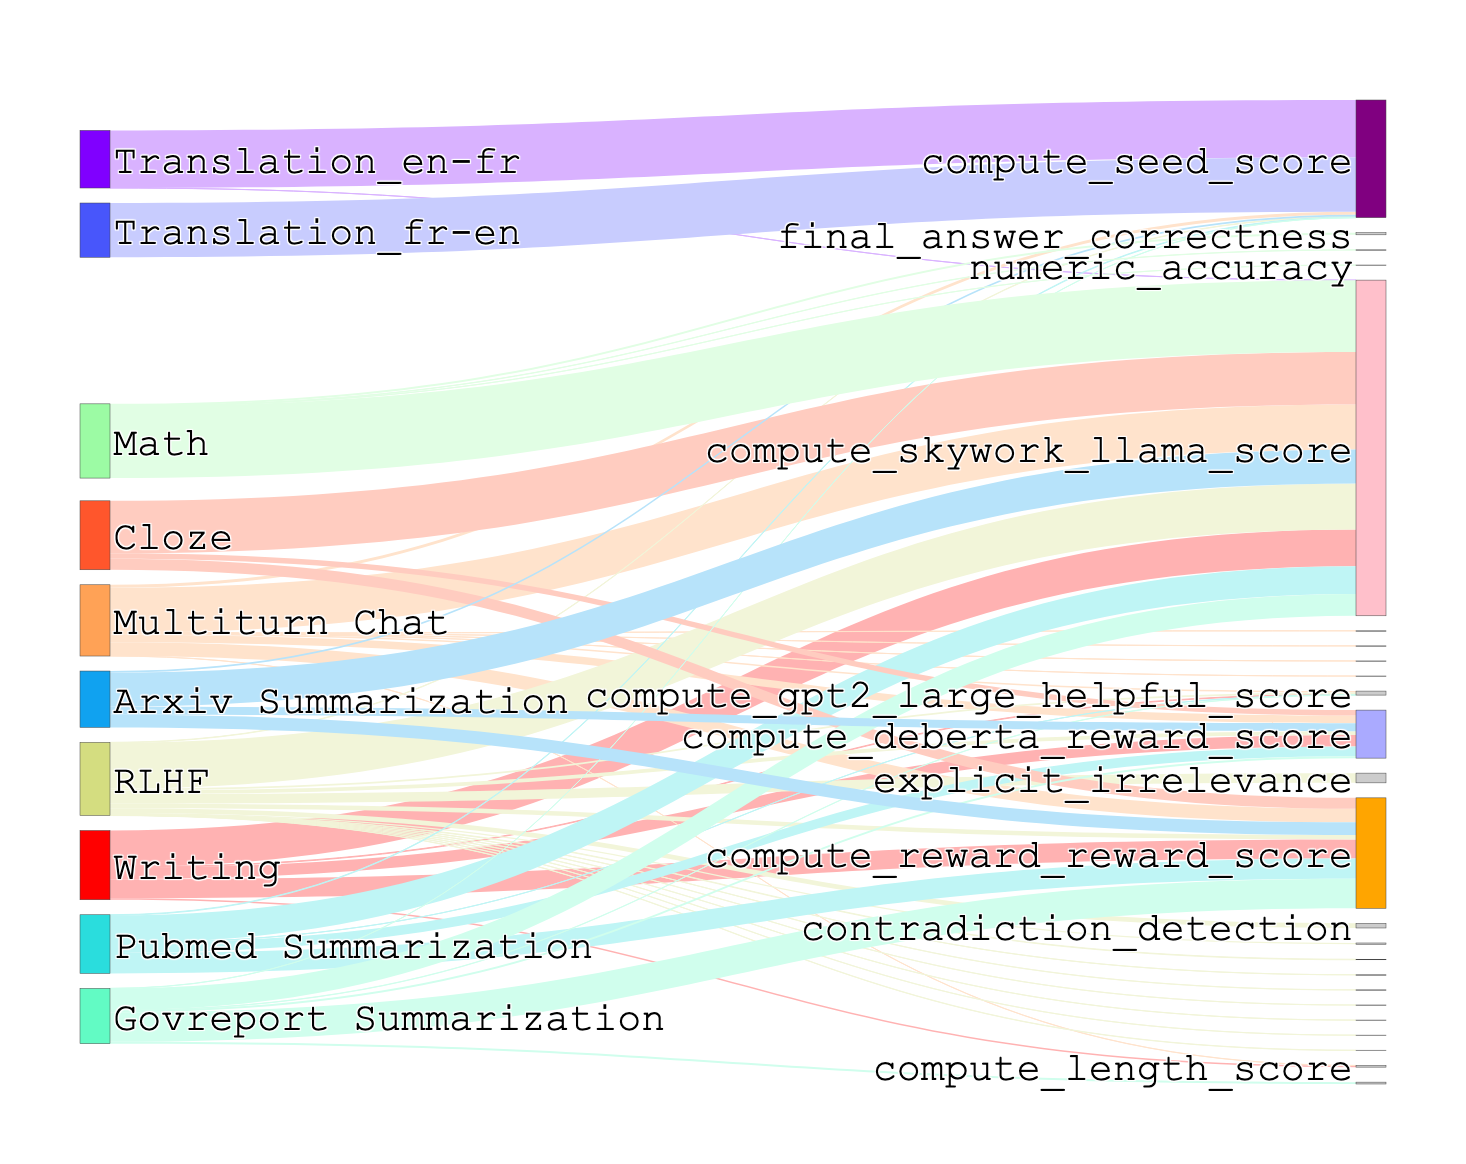
\includegraphics[width=0.45\textwidth]{Figures/sanky.png}
   \caption{Matching tools with source training dataset distribution.}
  \label{fig:sanky}
\end{figure}


The dominance of LLM-based rewards suggests that, for heterogeneous open-domain training, high-capacity discriminative models remain the most trusted. 
Nevertheless, the occasional use of rule-based checks in math and RLHF tasks demonstrates that \method{} is capable of \emph{combining expert heuristics} when appropriate.
\method{} does not rely on a single global reward model but instead orchestrates a \emph{portfolio} of evaluators aligned with each domain.
As shown in the previous subsection, this diversity translates into smoother advantage estimation and stronger updates during policy optimization.



\subsection{Impact on Advantage Estimation and Policy Learning}
% \subsection{Advantage Estimation: Generalists or Experts?


\begin{figure}[t]
    \centering
    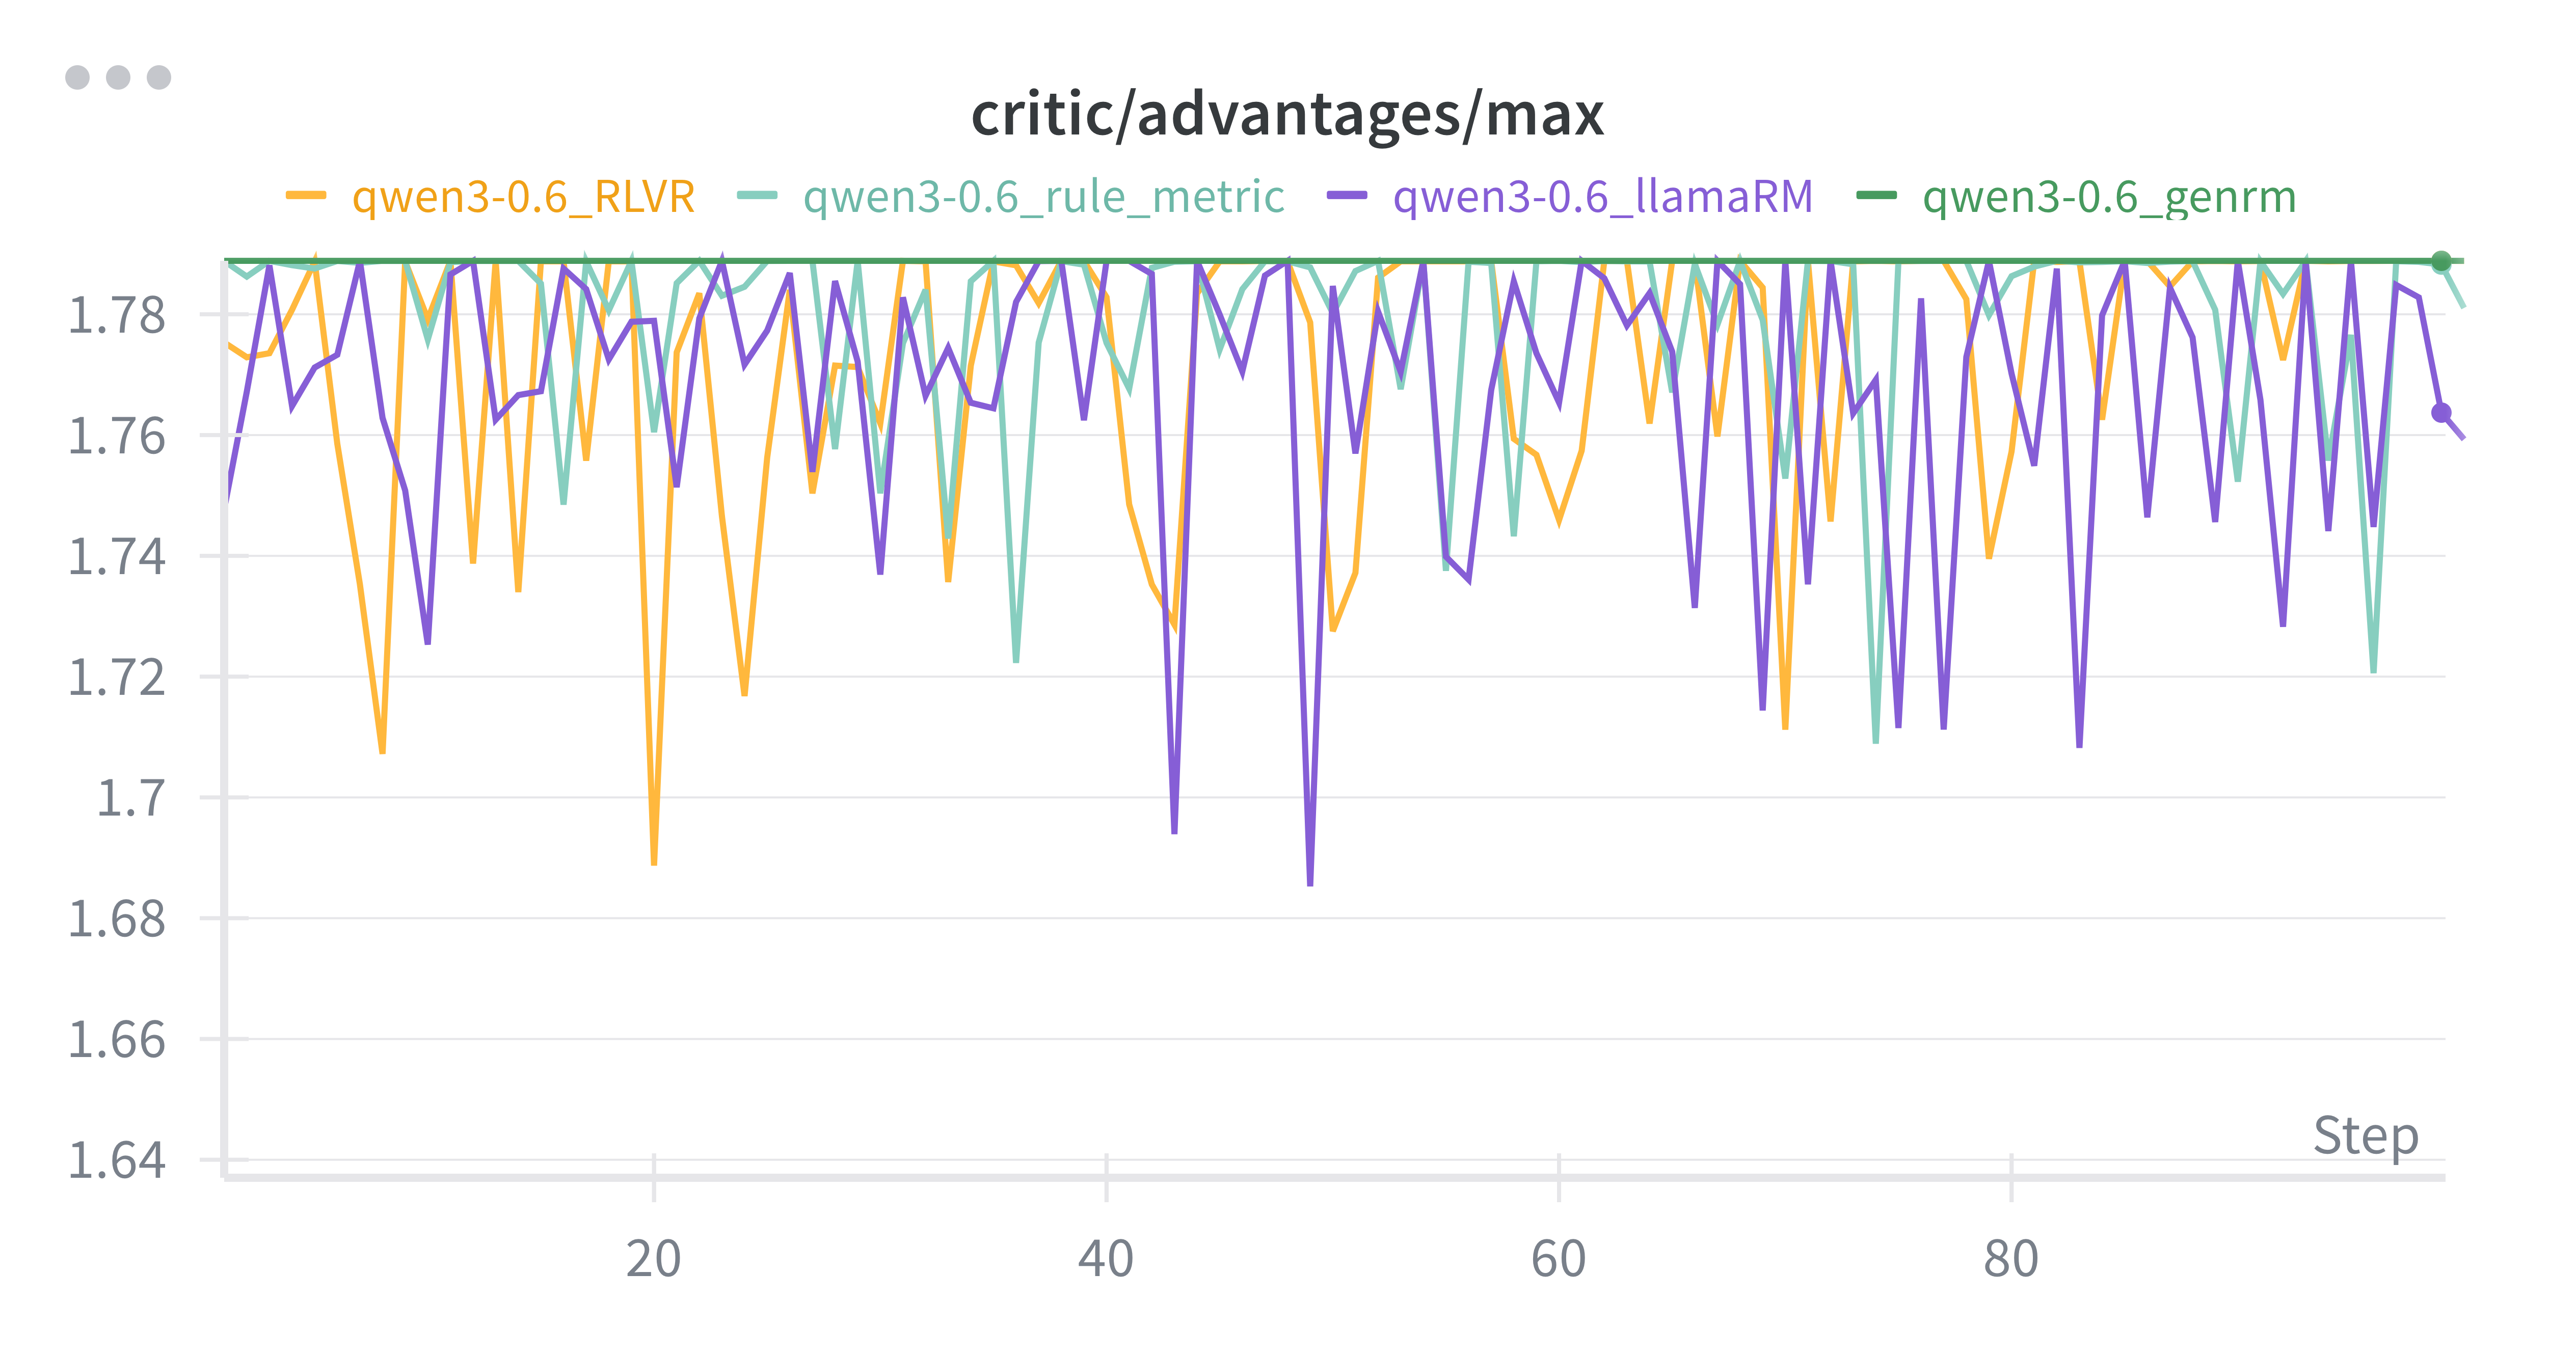
\includegraphics[width=1.0\linewidth]{Figures/adv_max_qwen.png}
    \caption{Maximum Advantage Estimations}
    \label{fig:max_adv}
\end{figure}

\begin{figure}[t]
    \centering
    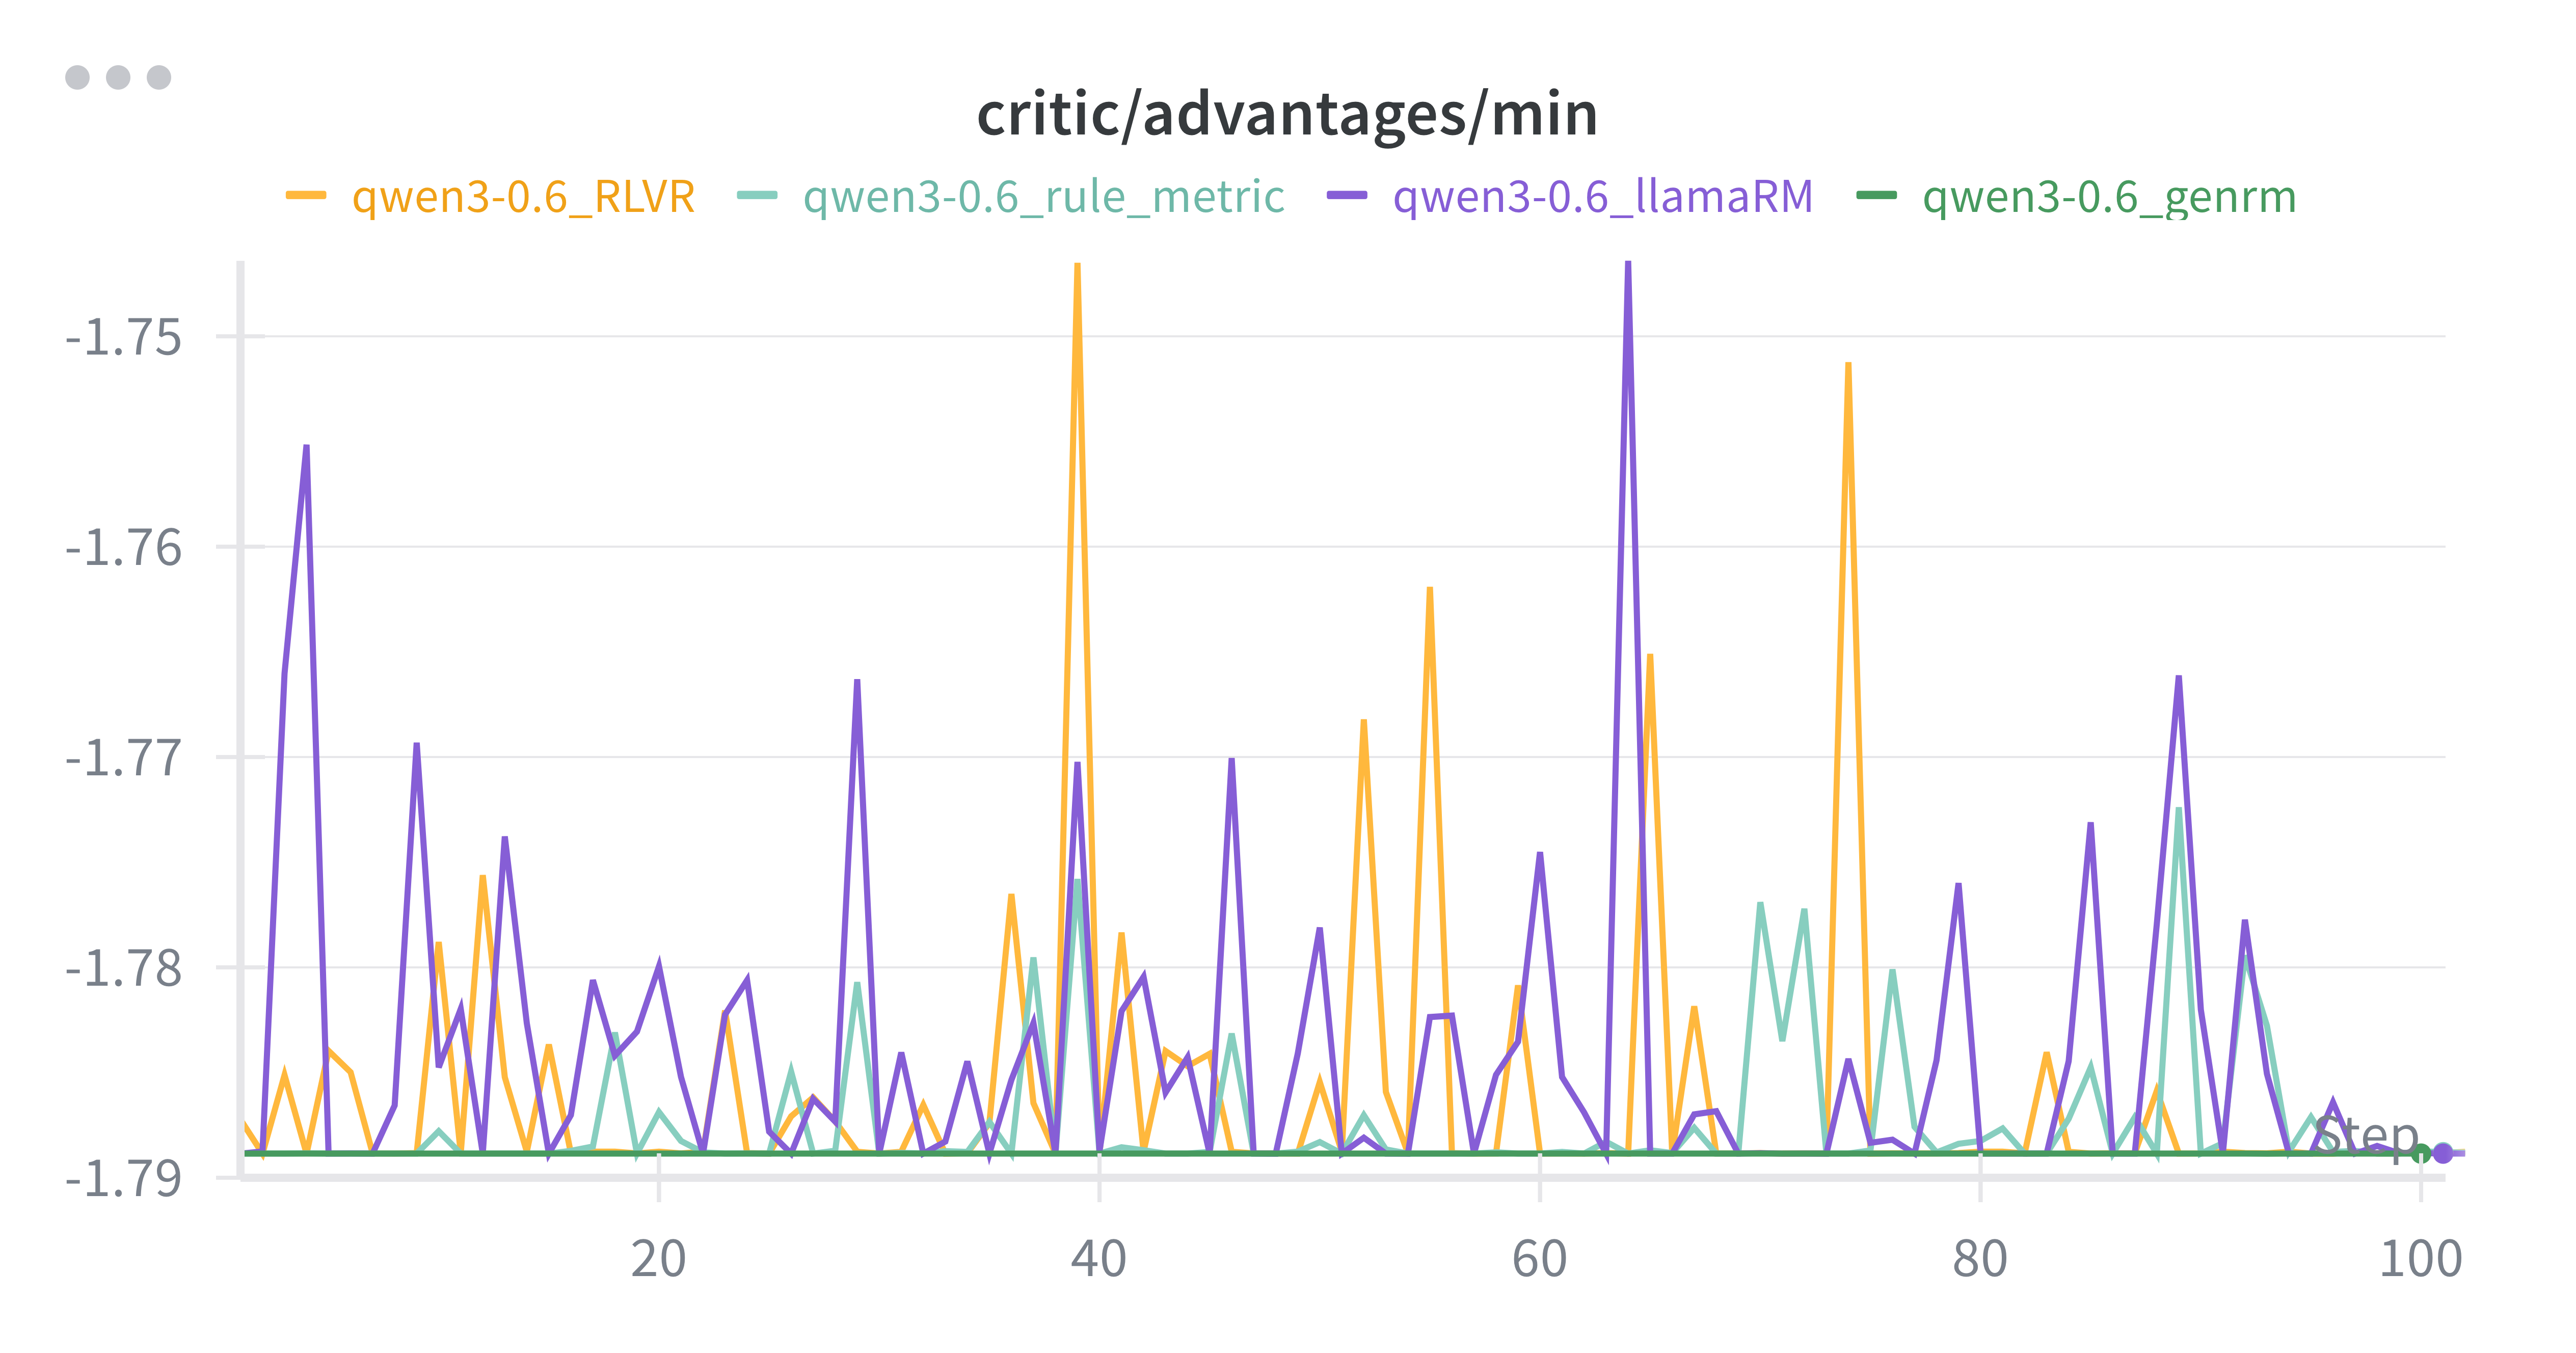
\includegraphics[width=1.0\linewidth]{Figures/adv_min_qwen.png}
    \caption{Minimum Advantage Estimations}
    \label{fig:min_adv}
\end{figure}


We examine the records from the Qwen experiments covering Generative RM, \method{}, and single generic reward, regarding the estimated min/max of advantage per step (Figure~\ref{fig:max_adv} and Figure~\ref{fig:min_adv}), and calculate the proportion that triggered clipping. Higher rates of being clipped mean a higher absolute value of estimated advantage. From the results, for Generative RM, rollouts triggering both upper-clip and under-clip occur in every update step. Compared to single generic reward, \method{} has a significantly higher clipping rate. This is direct evidence that \textbf{methods with better performance tend to estimate larger advantages in absolute values}.



\begin{figure}[t]
  \centering
  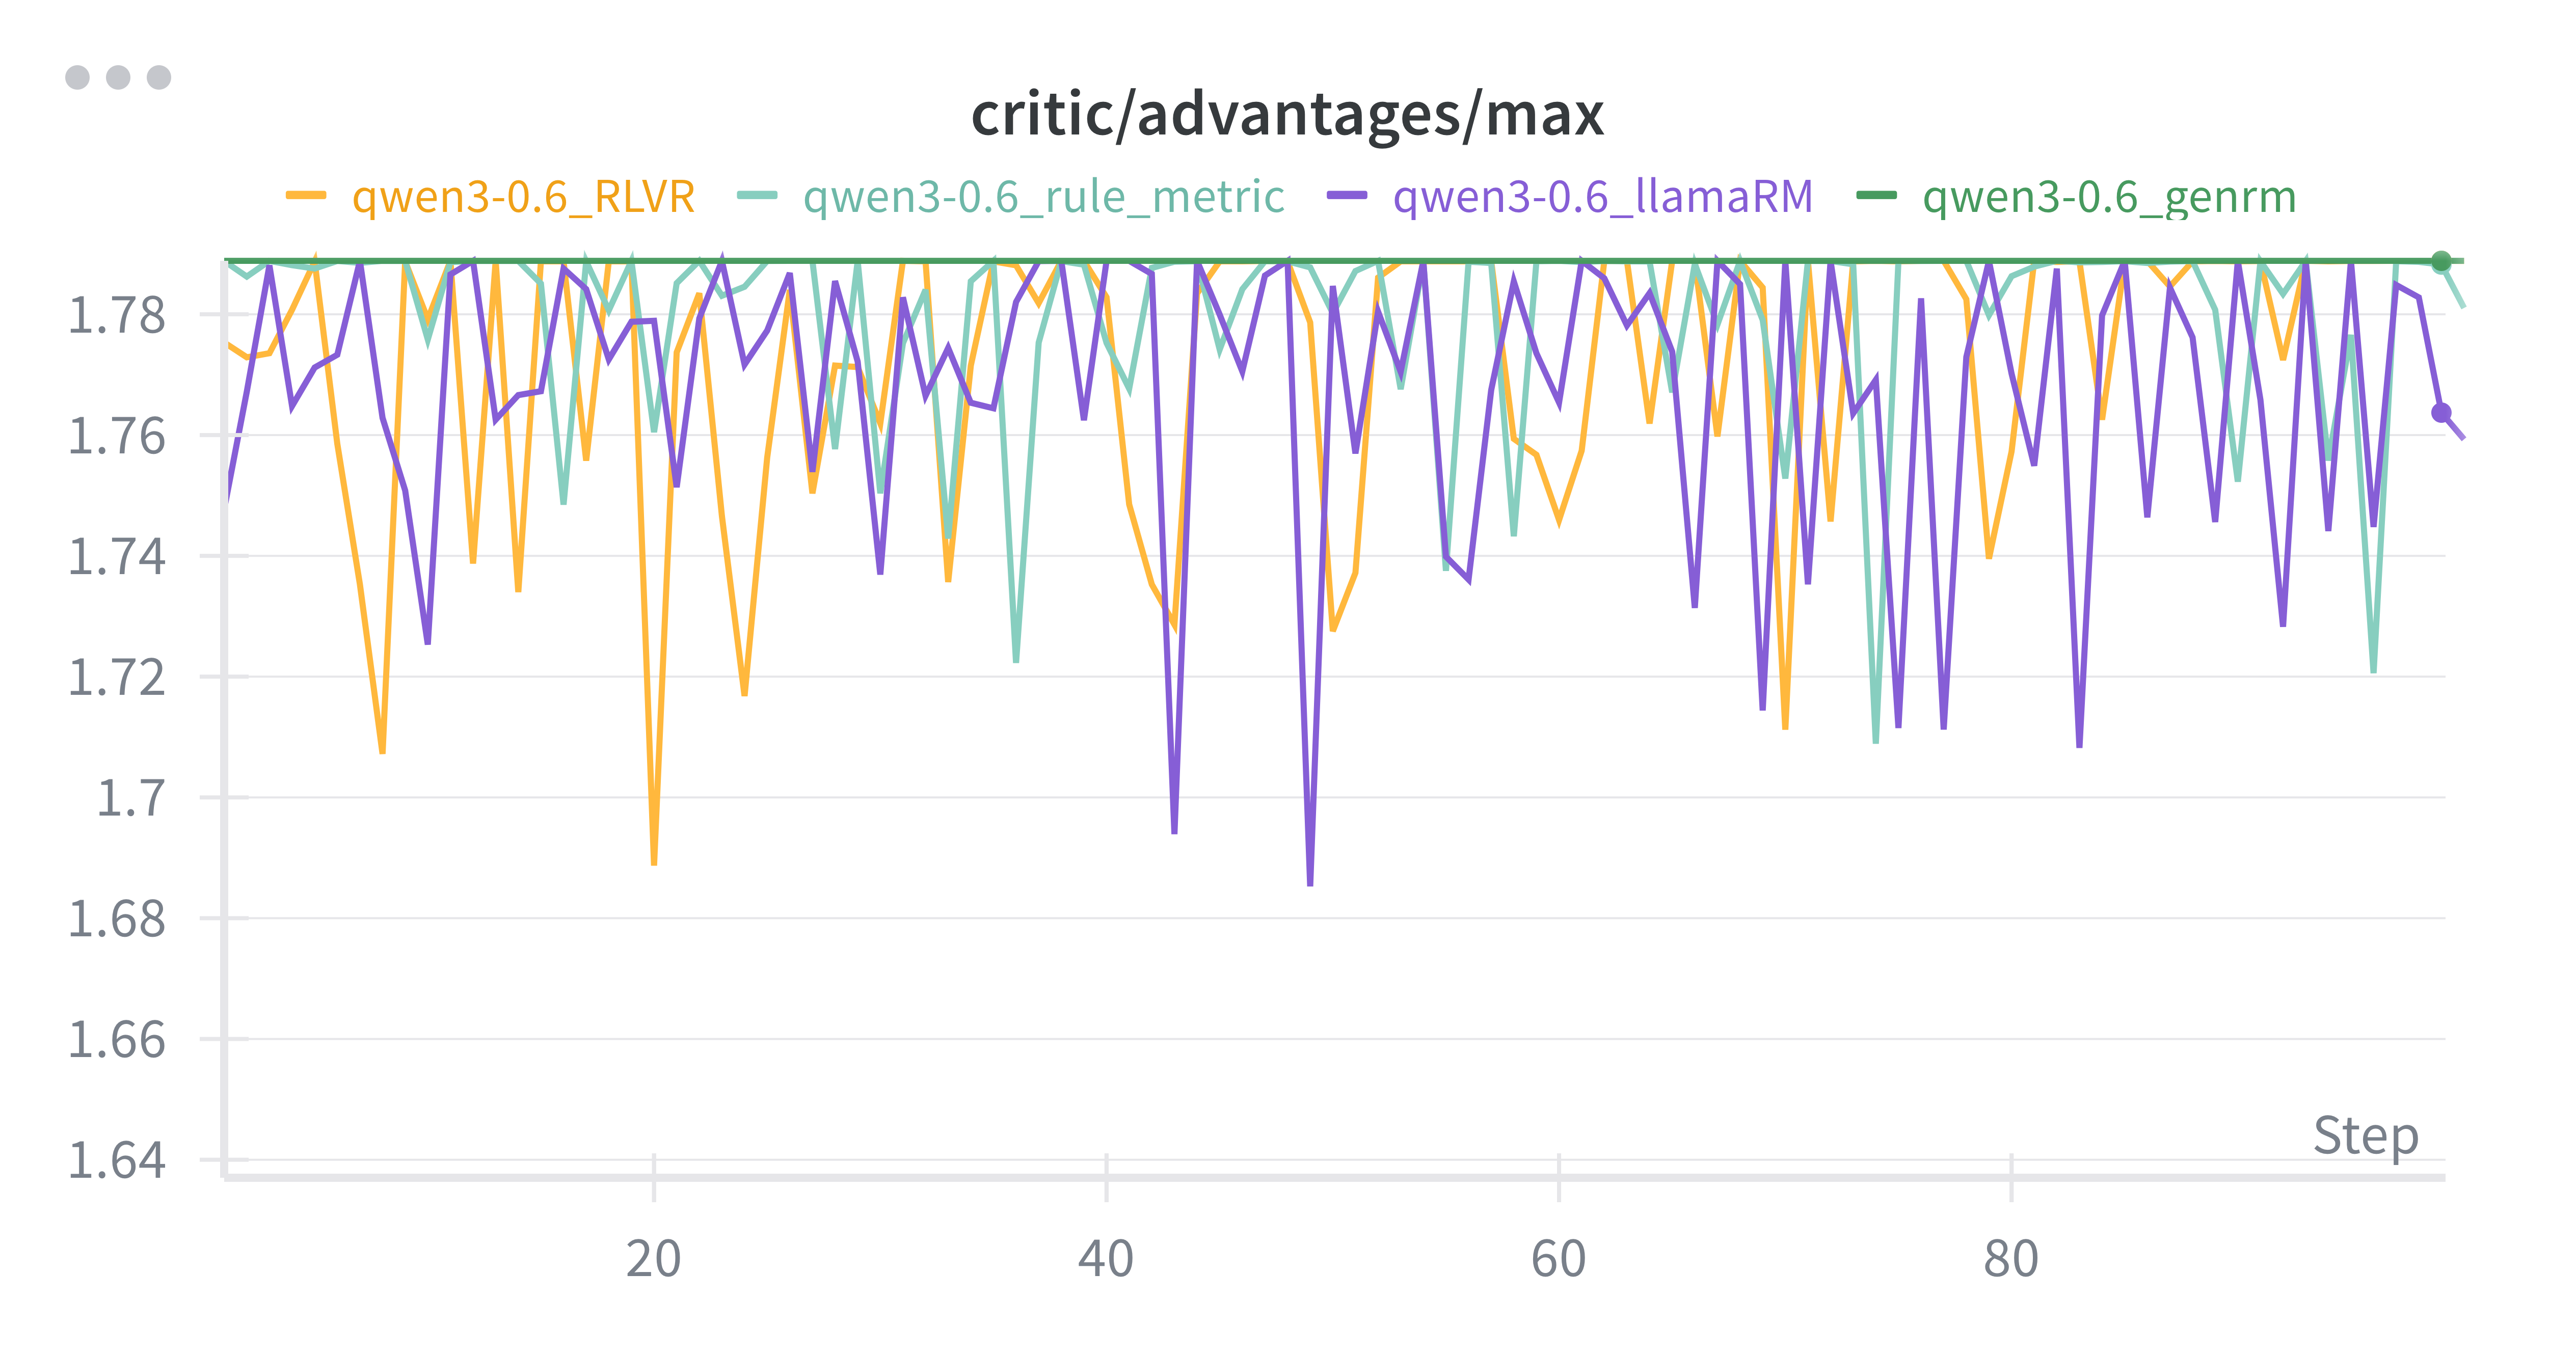
\includegraphics[width=1.0\linewidth]{Figures/adv_max_qwen.png}
   \caption{\small An illustration on the sensitivity to extreme values of reward functions.}
  \label{fig:illustrate}
\end{figure}


Returning to the discussion of Advantage Estimation \(\hat{A}_{i} = \frac{r_i - \mathrm{mean}(r)}{\mathrm{std}(r)}\). Consider two types of reward functions in Figure~\ref{fig:illustrate}: the blue one is sensitive to extreme values (smaller variance) while the orange one is evenly modeled (higher variance).
Assuming uniform roll-out sampling, a higher value of \(\hat{A}_i\) suggests that the underlying reward function resembles \textbf{the sensitive type} (blue line). Therefore, extreme values (maximum/minimum) are divided by a smaller variance, resulting in more frequent reaching of the clip threshold. This is expected for policy optimization, where more weight should be assigned to these deviated rollouts as part of the exploration-exploitation balance.








% \section{Technical appendices and supplementary material}
% Technical appendices with additional results, figures, graphs, and proofs may be submitted with the paper submission before the full submission deadline (see above). You can upload a ZIP file for videos or code, but do not upload a separate PDF file for the appendix. There is no page limit for the technical appendices. 

% Note: Think of the appendix as ``optional reading'' for reviewers. The paper must be able to stand alone without the appendix; for example, adding critical experiments that support the main claims to an appendix is inappropriate. 

%%%%%%%%%%%%%%%%%%%%%%%%%%%%%%%%%%%%%%%%%%%%%%%%%%%%%%%%%%%%

\newpage
\section*{NeurIPS Paper Checklist}


\begin{enumerate}

\item {\bf Claims}
    \item[] Question: Do the main claims made in the abstract and introduction accurately reflect the paper's contributions and scope?
    \item[] Answer: \answerYes{}
    \item[] Justification: The abstract and introduction clearly state our contributions of the proposal and design of \method{}.
    \item[] Guidelines:
    \begin{itemize}
        \item The answer \answerNA{} means that the abstract and introduction do not include the claims made in the paper.
        \item The abstract and/or introduction should clearly state the claims made, including the contributions made in the paper and important assumptions and limitations. A \answerNo{} or \answerNA{} answer to this question will not be perceived well by the reviewers. 
        \item The claims made should match theoretical and experimental results, and reflect how much the results can be expected to generalize to other settings. 
        \item It is fine to include aspirational goals as motivation as long as it is clear that these goals are not attained by the paper. 
    \end{itemize}

\item {\bf Limitations}
    \item[] Question: Does the paper discuss the limitations of the work performed by the authors?
    \item[] Answer: \answerYes{}
    \item[] Justification: We discuss the limitations in the Limitation Section.
    \item[] Guidelines:
    \begin{itemize}
        \item The answer \answerNA{} means that the paper has no limitation while the answer \answerNo{} means that the paper has limitations, but those are not discussed in the paper. 
        \item The authors are encouraged to create a separate ``Limitations'' section in their paper.
        \item The paper should point out any strong assumptions and how robust the results are to violations of these assumptions (e.g., independence assumptions, noiseless settings, model well-specification, asymptotic approximations only holding locally). The authors should reflect on how these assumptions might be violated in practice and what the implications would be.
        \item The authors should reflect on the scope of the claims made, e.g., if the approach was only tested on a few datasets or with a few runs. In general, empirical results often depend on implicit assumptions, which should be articulated.
        \item The authors should reflect on the factors that influence the performance of the approach. For example, a facial recognition algorithm may perform poorly when image resolution is low or images are taken in low lighting. Or a speech-to-text system might not be used reliably to provide closed captions for online lectures because it fails to handle technical jargon.
        \item The authors should discuss the computational efficiency of the proposed algorithms and how they scale with dataset size.
        \item If applicable, the authors should discuss possible limitations of their approach to address problems of privacy and fairness.
        \item While the authors might fear that complete honesty about limitations might be used by reviewers as grounds for rejection, a worse outcome might be that reviewers discover limitations that aren't acknowledged in the paper. The authors should use their best judgment and recognize that individual actions in favor of transparency play an important role in developing norms that preserve the integrity of the community. Reviewers will be specifically instructed to not penalize honesty concerning limitations.
    \end{itemize}

\item {\bf Theory assumptions and proofs}
    \item[] Question: For each theoretical result, does the paper provide the full set of assumptions and a complete (and correct) proof?
    \item[] Answer: \answerNA{} % Replace by \answerYes{}, \answerNo{}, or \answerNA{}.
    \item[] Justification: The paper focuses on empirical results and does not include formal theoretical claims.
    \item[] Guidelines:
    \begin{itemize}
        \item The answer \answerNA{} means that the paper does not include theoretical results. 
        \item All the theorems, formulas, and proofs in the paper should be numbered and cross-referenced.
        \item All assumptions should be clearly stated or referenced in the statement of any theorems.
        \item The proofs can either appear in the main paper or the supplemental material, but if they appear in the supplemental material, the authors are encouraged to provide a short proof sketch to provide intuition. 
        \item Inversely, any informal proof provided in the core of the paper should be complemented by formal proofs provided in appendix or supplemental material.
        \item Theorems and Lemmas that the proof relies upon should be properly referenced. 
    \end{itemize}

    \item {\bf Experimental result reproducibility}
    \item[] Question: Does the paper fully disclose all the information needed to reproduce the main experimental results of the paper to the extent that it affects the main claims and/or conclusions of the paper (regardless of whether the code and data are provided or not)?
    \item[] Answer: \answerYes{} % Replace by \answerYes{}, \answerNo{}, or \answerNA{}.
    \item[] Justification: We have included an anonymous GitHub URL containing the data and code for the experiments.
    \item[] Guidelines:
    \begin{itemize}
        \item The answer \answerNA{} means that the paper does not include experiments.
        \item If the paper includes experiments, a \answerNo{} answer to this question will not be perceived well by the reviewers: Making the paper reproducible is important, regardless of whether the code and data are provided or not.
        \item If the contribution is a dataset and\slash or model, the authors should describe the steps taken to make their results reproducible or verifiable. 
        \item Depending on the contribution, reproducibility can be accomplished in various ways. For example, if the contribution is a novel architecture, describing the architecture fully might suffice, or if the contribution is a specific model and empirical evaluation, it may be necessary to either make it possible for others to replicate the model with the same dataset, or provide access to the model. In general. releasing code and data is often one good way to accomplish this, but reproducibility can also be provided via detailed instructions for how to replicate the results, access to a hosted model (e.g., in the case of a large language model), releasing of a model checkpoint, or other means that are appropriate to the research performed.
        \item While NeurIPS does not require releasing code, the conference does require all submissions to provide some reasonable avenue for reproducibility, which may depend on the nature of the contribution. For example
        \begin{enumerate}
            \item If the contribution is primarily a new algorithm, the paper should make it clear how to reproduce that algorithm.
            \item If the contribution is primarily a new model architecture, the paper should describe the architecture clearly and fully.
            \item If the contribution is a new model (e.g., a large language model), then there should either be a way to access this model for reproducing the results or a way to reproduce the model (e.g., with an open-source dataset or instructions for how to construct the dataset).
            \item We recognize that reproducibility may be tricky in some cases, in which case authors are welcome to describe the particular way they provide for reproducibility. In the case of closed-source models, it may be that access to the model is limited in some way (e.g., to registered users), but it should be possible for other researchers to have some path to reproducing or verifying the results.
        \end{enumerate}
    \end{itemize}


\item {\bf Open access to data and code}
    \item[] Question: Does the paper provide open access to the data and code, with sufficient instructions to faithfully reproduce the main experimental results, as described in supplemental material?
    \item[] Answer: \answerYes{} % Replace by \answerYes{}, \answerNo{}, or \answerNA{}.
    \item[] Justification: We have included an anonymous GitHub URL containing the data and code for the experiments.
    \item[] Guidelines:
    \begin{itemize}
        \item The answer \answerNA{} means that paper does not include experiments requiring code.
        \item Please see the NeurIPS code and data submission guidelines (\url{https://neurips.cc/public/guides/CodeSubmissionPolicy}) for more details.
        \item While we encourage the release of code and data, we understand that this might not be possible, so \answerNo{} is an acceptable answer. Papers cannot be rejected simply for not including code, unless this is central to the contribution (e.g., for a new open-source benchmark).
        \item The instructions should contain the exact command and environment needed to run to reproduce the results. See the NeurIPS code and data submission guidelines (\url{https://neurips.cc/public/guides/CodeSubmissionPolicy}) for more details.
        \item The authors should provide instructions on data access and preparation, including how to access the raw data, preprocessed data, intermediate data, and generated data, etc.
        \item The authors should provide scripts to reproduce all experimental results for the new proposed method and baselines. If only a subset of experiments are reproducible, they should state which ones are omitted from the script and why.
        \item At submission time, to preserve anonymity, the authors should release anonymized versions (if applicable).
        \item Providing as much information as possible in supplemental material (appended to the paper) is recommended, but including URLs to data and code is permitted.
    \end{itemize}


\item {\bf Experimental setting/details}
    \item[] Question: Does the paper specify all the training and test details (e.g., data splits, hyperparameters, how they were chosen, type of optimizer) necessary to understand the results?
    \item[] Answer: \answerYes{} % Replace by \answerYes{}, \answerNo{}, or \answerNA{}.
    \item[] Justification: We have reported it in Section 5 and Appendix B, C.
    \item[] Guidelines:
    \begin{itemize}
        \item The answer \answerNA{} means that the paper does not include experiments.
        \item The experimental setting should be presented in the core of the paper to a level of detail that is necessary to appreciate the results and make sense of them.
        \item The full details can be provided either with the code, in appendix, or as supplemental material.
    \end{itemize}

\item {\bf Experiment statistical significance}
    \item[] Question: Does the paper report error bars suitably and correctly defined or other appropriate information about the statistical significance of the experiments?
    \item[] Answer: \answerNo{} % Replace by \answerYes{}, \answerNo{}, or \answerNA{}.
    \item[] Justification: No, due to the extreme computational cost of training the LLM/API, results are based on a single run.
    \item[] Guidelines:
    \begin{itemize}
        \item The answer \answerNA{} means that the paper does not include experiments.
        \item The authors should answer \answerYes{} if the results are accompanied by error bars, confidence intervals, or statistical significance tests, at least for the experiments that support the main claims of the paper.
        \item The factors of variability that the error bars are capturing should be clearly stated (for example, train/test split, initialization, random drawing of some parameter, or overall run with given experimental conditions).
        \item The method for calculating the error bars should be explained (closed form formula, call to a library function, bootstrap, etc.)
        \item The assumptions made should be given (e.g., Normally distributed errors).
        \item It should be clear whether the error bar is the standard deviation or the standard error of the mean.
        \item It is OK to report 1-sigma error bars, but one should state it. The authors should preferably report a 2-sigma error bar than state that they have a 96\% CI, if the hypothesis of Normality of errors is not verified.
        \item For asymmetric distributions, the authors should be careful not to show in tables or figures symmetric error bars that would yield results that are out of range (e.g., negative error rates).
        \item If error bars are reported in tables or plots, the authors should explain in the text how they were calculated and reference the corresponding figures or tables in the text.
    \end{itemize}

\item {\bf Experiments compute resources}
    \item[] Question: For each experiment, does the paper provide sufficient information on the computer resources (type of compute workers, memory, time of execution) needed to reproduce the experiments?
    \item[] Answer: \answerYes{} % Replace by \answerYes{}, \answerNo{}, or \answerNA{}.
    \item[] Justification: We have disclosed the computation resources in Appendix C.1.
    \item[] Guidelines:
    \begin{itemize}
        \item The answer \answerNA{} means that the paper does not include experiments.
        \item The paper should indicate the type of compute workers CPU or GPU, internal cluster, or cloud provider, including relevant memory and storage.
        \item The paper should provide the amount of compute required for each of the individual experimental runs as well as estimate the total compute. 
        \item The paper should disclose whether the full research project required more compute than the experiments reported in the paper (e.g., preliminary or failed experiments that didn't make it into the paper). 
    \end{itemize}
    
\item {\bf Code of ethics}
    \item[] Question: Does the research conducted in the paper conform, in every respect, with the NeurIPS Code of Ethics \url{https://neurips.cc/public/EthicsGuidelines}?
    \item[] Answer: \answerYes{} % Replace by \answerYes{}, \answerNo{}, or \answerNA{}.
    \item[] Justification: We have ensured the anonymity. For the reward models involved in this research, there are publicly available on Huggingface and their licenses ensure the development for Generative Artificial Intelligence.
    \item[] Guidelines:
    \begin{itemize}
        \item The answer \answerNA{} means that the authors have not reviewed the NeurIPS Code of Ethics.
        \item If the authors answer \answerNo, they should explain the special circumstances that require a deviation from the Code of Ethics.
        \item The authors should make sure to preserve anonymity (e.g., if there is a special consideration due to laws or regulations in their jurisdiction).
    \end{itemize}


\item {\bf Broader impacts}
    \item[] Question: Does the paper discuss both potential positive societal impacts and negative societal impacts of the work performed?
    \item[] Answer: \answerYes{}{} % Replace by \answerYes{}, \answerNo{}, or \answerNA{}.
    \item[] Justification: Yes, we have discussed in Section~\ref{sec:impact_ethic}.
    \item[] Guidelines:
    \begin{itemize}
        \item The answer \answerNA{} means that there is no societal impact of the work performed.
        \item If the authors answer \answerNA{} or \answerNo, they should explain why their work has no societal impact or why the paper does not address societal impact.
        \item Examples of negative societal impacts include potential malicious or unintended uses (e.g., disinformation, generating fake profiles, surveillance), fairness considerations (e.g., deployment of technologies that could make decisions that unfairly impact specific groups), privacy considerations, and security considerations.
        \item The conference expects that many papers will be foundational research and not tied to particular applications, let alone deployments. However, if there is a direct path to any negative applications, the authors should point it out. For example, it is legitimate to point out that an improvement in the quality of generative models could be used to generate Deepfakes for disinformation. On the other hand, it is not needed to point out that a generic algorithm for optimizing neural networks could enable people to train models that generate Deepfakes faster.
        \item The authors should consider possible harms that could arise when the technology is being used as intended and functioning correctly, harms that could arise when the technology is being used as intended but gives incorrect results, and harms following from (intentional or unintentional) misuse of the technology.
        \item If there are negative societal impacts, the authors could also discuss possible mitigation strategies (e.g., gated release of models, providing defenses in addition to attacks, mechanisms for monitoring misuse, mechanisms to monitor how a system learns from feedback over time, improving the efficiency and accessibility of ML).
    \end{itemize}
    
\item {\bf Safeguards}
    \item[] Question: Does the paper describe safeguards that have been put in place for responsible release of data or models that have a high risk for misuse (e.g., pre-trained language models, image generators, or scraped datasets)?
    \item[] Answer: \answerYes{}{} % Replace by \answerYes{}, \answerNo{}, or \answerNA{}.
    \item[] Justification: Yes, we have discussed in Section~\ref{sec:impact_ethic}.
    \item[] Guidelines:
    \begin{itemize}
        \item The answer \answerNA{} means that the paper poses no such risks.
        \item Released models that have a high risk for misuse or dual-use should be released with necessary safeguards to allow for controlled use of the model, for example by requiring that users adhere to usage guidelines or restrictions to access the model or implementing safety filters. 
        \item Datasets that have been scraped from the Internet could pose safety risks. The authors should describe how they avoided releasing unsafe images.
        \item We recognize that providing effective safeguards is challenging, and many papers do not require this, but we encourage authors to take this into account and make a best faith effort.
    \end{itemize}

\item {\bf Licenses for existing assets}
    \item[] Question: Are the creators or original owners of assets (e.g., code, data, models), used in the paper, properly credited and are the license and terms of use explicitly mentioned and properly respected?
    \item[] Answer: \answerYes{} % Replace by \answerYes{}, \answerNo{}, or \answerNA{}.
    \item[] Justification: Yes, we have rechecked the licenses and make sure that the usage of Huggingface model checkpoints to conduct this research is proper.
    \item[] Guidelines:
    \begin{itemize}
        \item The answer \answerNA{} means that the paper does not use existing assets.
        \item The authors should cite the original paper that produced the code package or dataset.
        \item The authors should state which version of the asset is used and, if possible, include a URL.
        \item The name of the license (e.g., CC-BY 4.0) should be included for each asset.
        \item For scraped data from a particular source (e.g., website), the copyright and terms of service of that source should be provided.
        \item If assets are released, the license, copyright information, and terms of use in the package should be provided. For popular datasets, \url{paperswithcode.com/datasets} has curated licenses for some datasets. Their licensing guide can help determine the license of a dataset.
        \item For existing datasets that are re-packaged, both the original license and the license of the derived asset (if it has changed) should be provided.
        \item If this information is not available online, the authors are encouraged to reach out to the asset's creators.
    \end{itemize}

\item {\bf New assets}
    \item[] Question: Are new assets introduced in the paper well documented and is the documentation provided alongside the assets?
    \item[] Answer: \answerYes{} % Replace by \answerYes{}, \answerNo{}, or \answerNA{}.
    \item[] Justification: Yes, we have provided a readme in the given anonymous GitHub URL.
    \item[] Guidelines:
    \begin{itemize}
        \item The answer \answerNA{} means that the paper does not release new assets.
        \item Researchers should communicate the details of the dataset\slash code\slash model as part of their submissions via structured templates. This includes details about training, license, limitations, etc. 
        \item The paper should discuss whether and how consent was obtained from people whose asset is used.
        \item At submission time, remember to anonymize your assets (if applicable). You can either create an anonymized URL or include an anonymized zip file.
    \end{itemize}

\item {\bf Crowdsourcing and research with human subjects}
    \item[] Question: For crowdsourcing experiments and research with human subjects, does the paper include the full text of instructions given to participants and screenshots, if applicable, as well as details about compensation (if any)? 
    \item[] Answer: \answerNA{} % Replace by \answerYes{}, \answerNo{}, or \answerNA{}.
    \item[] Justification: We did not include crowdsourcing experiments or research with human subjects.
    \item[] Guidelines:
    \begin{itemize}
        \item The answer \answerNA{} means that the paper does not involve crowdsourcing nor research with human subjects.
        \item Including this information in the supplemental material is fine, but if the main contribution of the paper involves human subjects, then as much detail as possible should be included in the main paper. 
        \item According to the NeurIPS Code of Ethics, workers involved in data collection, curation, or other labor should be paid at least the minimum wage in the country of the data collector. 
    \end{itemize}

\item {\bf Institutional review board (IRB) approvals or equivalent for research with human subjects}
    \item[] Question: Does the paper describe potential risks incurred by study participants, whether such risks were disclosed to the subjects, and whether Institutional Review Board (IRB) approvals (or an equivalent approval/review based on the requirements of your country or institution) were obtained?
    \item[] Answer: \answerNA{} % Replace by \answerYes{}, \answerNo{}, or \answerNA{}.
    \item[] Justification: We did not include crowdsourcing experiments or research with human subjects.
    \item[] Guidelines:
    \begin{itemize}
        \item The answer \answerNA{} means that the paper does not involve crowdsourcing nor research with human subjects.
        \item Depending on the country in which research is conducted, IRB approval (or equivalent) may be required for any human subjects research. If you obtained IRB approval, you should clearly state this in the paper. 
        \item We recognize that the procedures for this may vary significantly between institutions and locations, and we expect authors to adhere to the NeurIPS Code of Ethics and the guidelines for their institution. 
        \item For initial submissions, do not include any information that would break anonymity (if applicable), such as the institution conducting the review.
    \end{itemize}

\item {\bf Declaration of LLM usage}
    \item[] Question: Does the paper describe the usage of LLMs if it is an important, original, or non-standard component of the core methods in this research? Note that if the LLM is used only for writing, editing, or formatting purposes and does \emph{not} impact the core methodology, scientific rigor, or originality of the research, declaration is not required.
    %this research? 
    \item[] Answer: \answerYes{} % Replace by \answerYes{}, \answerNo{}, or \answerNA{}.
    \item[] Justification: Yes, we have included the discussion in Appendix~\ref{apd:llm_usage}, that LLM is used as writing assistant for grammar/typo inspection. LLM itself is also the objective in this research.
    \item[] Guidelines:
    \begin{itemize}
        \item The answer \answerNA{} means that the core method development in this research does not involve LLMs as any important, original, or non-standard components.
        \item Please refer to our LLM policy in the NeurIPS handbook for what should or should not be described.
    \end{itemize}

\end{enumerate}


\end{document}

